%%% DOCUMENT TYPE %%%%%%%%%%%%%%%%%%%%%%%%%%%%%%%%%%%%%%%%%%%%%%%%%%%%%%%%%%%%%%

\documentclass[10pt, a4paper]{article}

%%% PACKAGES %%%%%%%%%%%%%%%%%%%%%%%%%%%%%%%%%%%%%%%%%%%%%%%%%%%%%%%%%%%%%%%%%%%

% Encoding

\usepackage[utf8]{inputenc}
\usepackage[T1]{fontenc}

% Geometry

\usepackage{geometry} % edit margins of paper
\usepackage{setspace} % edit line spacing
\usepackage{fancyhdr} % header, footer
\usepackage{titlesec} % edit format of titles

% Visual

\usepackage[dvipsnames]{xcolor} % colors
\usepackage{tikz} % graphics
\usepackage[framemethod=tikz]{mdframed} % frames, better theorems

% Math

\usepackage{amsmath} % math tools
\usepackage{amssymb} % math symbols
\usepackage{amsthm} % thereoms
\usepackage{mathtools} % math tools

% Referencing

\usepackage{nameref}
\usepackage{hyperref}
\usepackage{cleveref}

% Useful

\usepackage[shortlabels]{enumitem} % enumerations

% Other

\usepackage{lastpage} % get number of last page

%%% MARGINS %%%%%%%%%%%%%%%%%%%%%%%%%%%%%%%%%%%%%%%%%%%%%%%%%%%%%%%%%%%%%%%%%%%%

\geometry{a4paper, left=20mm, right=20mm, top=20mm, bottom=20mm, includehead}

%%% COLORS %%%%%%%%%%%%%%%%%%%%%%%%%%%%%%%%%%%%%%%%%%%%%%%%%%%%%%%%%%%%%%%%%%%%%

%%% TITLES %%%%%%%%%%%%%%%%%%%%%%%%%%%%%%%%%%%%%%%%%%%%%%%%%%%%%%%%%%%%%%%%%%%%%

\colorlet{color-section}                {BrickRed}
\colorlet{color-subsection}             {BrickRed}

%%% MATH BOXES %%%%%%%%%%%%%%%%%%%%%%%%%%%%%%%%%%%%%%%%%%%%%%%%%%%%%%%%%%%%%%%%%

\colorlet{color-definition}             {SpringGreen!20}
\colorlet{color-theorem}                {Apricot!13}
\colorlet{color-proposition}            {Apricot!13}
\colorlet{color-corollary}              {Apricot!13}
\colorlet{color-lemma}                  {Apricot!13}
\colorlet{color-remark}                 {Gray!5}
\colorlet{color-example}                {Lavender!7}
% \colorlet{color-proof}                  {FILL COLOR HERE}


%%% CAPTIONS %%%%%%%%%%%%%%%%%%%%%%%%%%%%%%%%%%%%%%%%%%%%%%%%%%%%%%%%%%%%%%%%%%%

%%% CAPTION DEFINITION %%%%%%%%%%%%%%%%%%%%%%%%%%%%%%%%%%%%%%%%%%%%%%%%%%%%%%%%%

\newcommand*{\definitionname}{Definition}
\newcommand*{\theoremname}{Theorem}
\newcommand*{\propositionname}{Proposition}
\newcommand*{\corollaryname}{Corollary}
\newcommand*{\lemmaname}{Lemma}
\newcommand*{\remarkname}{Remark}
\newcommand*{\examplename}{Example}


%%% SHORTCUTS %%%%%%%%%%%%%%%%%%%%%%%%%%%%%%%%%%%%%%%%%%%%%%%%%%%%%%%%%%%%%%%%%%

%%% SINGLE SYMBOLS %%%%%%%%%%%%%%%%%%%%%%%%%%%%%%%%%%%%%%%%%%%%%%%%%%%%%%%%%%%%

% Logic

% \forall exists
% \exists exists
% \lnot exists
% \lor exists
% \land exists
\newcommand*{\limp}{\rightarrow}
\newcommand*{\limps}{\; \limp \;} % \limp with some space around
\newcommand*{\leqv}{\leftrightarrow}
\newcommand*{\leqvs}{\; \leqvs \;} % \leqv with some space around

% Meta Logic

% \implies exists
% \iff exists

% Colon Stuff

\newcommand*{\cl}{\colon}
\newcommand*{\cleq}{\coloneqq}
\newcommand*{\eqcl}{\eqqcolon}

% Sets

\newcommand*{\N}{\mathbb{N}} % natural numbers
\newcommand*{\Z}{\mathbb{Z}} % integers
\newcommand*{\Q}{\mathbb{Q}} % rational numbers
\newcommand*{\R}{\mathbb{R}} % real numbers
%\newcommand*{\C}{\mathbb{C}} % complex numbers

%%% MATH OPERATORS %%%%%%%%%%%%%%%%%%%%%%%%%%%%%%%%%%%%%%%%%%%%%%%%%%%%%%%%%%%%%

% General

\DeclareMathOperator{\id}{id}
\DeclareMathOperator{\sgn}{sgn}

%%% TEMPLATES %%%%%%%%%%%%%%%%%%%%%%%%%%%%%%%%%%%%%%%%%%%%%%%%%%%%%%%%%%%%%%%%%%

% General

% write a set definition like: { #1 | #2 }
\newcommand*{\setdefinition}[2]{
  \left\{ #1 \mathrel{}\middle|\mathrel{} #2 \right\}
}

% write a nice map definition
\newcommand*{\mapdefinition}[5]{
  \begin{align*}
    #1 \cl #2 &\to     #3 \\
           #4 &\mapsto #5
  \end{align*}
}


%%% FORMATTING %%%%%%%%%%%%%%%%%%%%%%%%%%%%%%%%%%%%%%%%%%%%%%%%%%%%%%%%%%%%%%%%%

%%% HEADER, FOOTER %%%%%%%%%%%%%%%%%%%%%%%%%%%%%%%%%%%%%%%%%%%%%%%%%%%%%%%%%%%%%

\pagestyle{fancy}
\fancyhf{} % clear everything
\lhead{\sffamily maplgebra}
\chead{\sffamily \large \bfseries Topology}
\rhead{\sffamily Page \thepage /\pageref*{LastPage}}
\lfoot{}
\cfoot{}
\rfoot{}

%%% TITLE FORMAT %%%%%%%%%%%%%%%%%%%%%%%%%%%%%%%%%%%%%%%%%%%%%%%%%%%%%%%%%%%%%%%

\setcounter{secnumdepth}{2}

\titleformat{\chapter}[display]
{\normalfont\huge\bfseries}{\chaptertitlename\ \thechapter}{20pt}{\Huge}
\titleformat{\section}[frame]
{\normalfont\LARGE\bfseries\color{color-section}\scshape}{\filright\,\thesection\,}{0.2ex}{\filcenter}
\titleformat{\subsection}
{\normalfont\Large\bfseries\color{color-subsection}}{\thesubsection}{1em}{}
\titleformat{\subsubsection}
{\normalfont\normalsize\bfseries}{\thesubsubsection}{1em}{}
\titleformat{\paragraph}[runin]
{\normalfont\normalsize\bfseries}{\theparagraph}{1em}{}
\titleformat{\subparagraph}[runin]
{\normalfont\normalsize\bfseries}{\thesubparagraph}{1em}{}

%%% SPACING %%%%%%%%%%%%%%%%%%%%%%%%%%%%%%%%%%%%%%%%%%%%%%%%%%%%%%%%%%%%%%

% Titles

\titlespacing*{\chapter}{0pt}{50pt}{40pt}
\titlespacing*{\section}{0pt}{3.5ex plus 1ex minus .2ex}{2.3ex plus .2ex}
\titlespacing*{\subsection}{0pt}{3.25ex plus 1ex minus .2ex}{1.5ex plus .2ex}
\titlespacing*{\subsubsection}{0pt}{3.25ex plus 1ex minus .2ex}{1.5ex plus .2ex}
\titlespacing*{\paragraph}{0pt}{3.25ex plus 1ex minus .2ex}{1em}
\titlespacing*{\subparagraph}{\parindent}{3.25ex plus 1ex minus .2ex}{1em}

% Text, Paragraphs

%\setstretch{1.05} % scaling of space between lines
\setlength{\parindent}{0pt} % indentation of paragraphs
%\setlength{\parskip}{4.0pt plus 1.0pt minus 1.0pt} % space between paragraphs
\setlength{\parskip}{0.8ex}
\setlength{\topsep}{0pt}

%%% SYMBOLS USED BY NUMBERINGS, ENVIRONMENTS, ... %%%%%%%%%%%%%%%%%%%%%%%%%%%%%%

% \renewcommand*\qedsymbol{$\blacksquare$} % alternative QED symbol
\renewcommand{\thefootnote}{\arabic{footnote}} % normal footnotes on page
\renewcommand{\thempfootnote}{\fnsymbol{mpfootnote}} % footnotes on minipages, e.g. in mdframed environments

%%% LISTS, ENUMERATIONS %%%%%%%%%%%%%%%%%%%%%%%%%%%%%%%%%%%%%%%%%%%%%%%%%%%%%%%%

% 'itemize'

\setlist[itemize]{noitemsep, topsep=0pt}

% 'enumerate'

% no special settings at the moment

% 'description'

% no special settings at the moment

% 'axioms'

\newlist{axioms}{enumerate}{2}
\setlist[axioms]{itemsep=0pt,label*=\arabic*.}

%%% MDFRAMED PATCH %%%%%%%%%%%%%%%%%%%%%%%%%%%%%%%%%%%%%%%%%%%%%%%%%%%%%%%%%%%%%

\usepackage{xpatch}

\makeatletter
\xpatchcmd{\endmdframed}
  {\aftergroup\endmdf@trivlist\color@endgroup}
  {\endmdf@trivlist\color@endgroup\@doendpe}
  {}{}
\makeatother

%%% MDFRAMED STYLES %%%%%%%%%%%%%%%%%%%%%%%%%%%%%%%%%%%%%%%%%%%%%%%%%%%%%%%%%%%%

% thick frame and bar for title

\mdfdefinestyle{style-box}{
  skipabove=1.5ex plus .5ex minus .2ex,
  skipbelow=1ex plus .2ex minus .2ex,
  linewidth=2pt,
  linecolor=Gray!20,
%   roundcorner=3pt,
  innerleftmargin=0.5\baselineskip,
  innerrightmargin=0.5\baselineskip,
  innertopmargin=0.4\baselineskip,
  innerbottommargin=0.4\baselineskip,
  frametitlebackgroundcolor=Gray!20,
  frametitleaboveskip=0.3pt,
  frametitlebelowskip=0.3pt,
  theoremseparator=,
  theoremspace=\hfill,
  theoremtitlefont=\mdseries\scshape,
  nobreak=true
}

% highlighted background

\mdfdefinestyle{style-background}{
  skipabove=1.5ex plus .5ex minus .2ex,
  skipbelow=1ex plus .2ex minus .2ex,
  hidealllines=true,
  backgroundcolor=Gray!5,
  innerleftmargin=0.5\baselineskip,
  innerrightmargin=0.5\baselineskip,
  innertopmargin=0.4\baselineskip,
  innerbottommargin=0.4\baselineskip,
}

% thin frame

\mdfdefinestyle{style-leftline}{
  skipabove=1.5ex plus .5ex minus .2ex,
  skipbelow=1ex plus .2ex minus .2ex,
  linewidth=1pt,
  linecolor=Gray!50,
  topline=false,
  bottomline=false,
  rightline=false,
  innerleftmargin=0.5\baselineskip,
  innerrightmargin=0,
  innertopmargin=0.2\baselineskip,
  innerbottommargin=0.0\baselineskip,
}

%%% ENVIRONMENTS %%%%%%%%%%%%%%%%%%%%%%%%%%%%%%%%%%%%%%%%%%%%%%%%%%%%%%%%%%%%%%%

% Definition

\mdtheorem[
  style=style-box,
  linecolor=color-definition,
  frametitlebackgroundcolor=color-definition
]{definition}{\definitionname}[section]

% Theorem

\mdtheorem[
  style=style-box,
  linecolor=color-theorem,
  frametitlebackgroundcolor=color-theorem,
  font=\itshape
]{theorem}{\theoremname}[section]

% Proposition

\mdtheorem[
  style=style-box,
  linecolor=color-proposition,
  frametitlebackgroundcolor=color-proposition,
  font=\itshape
]{proposition}[theorem]{\propositionname}

% Corollary

\mdtheorem[
  style=style-box,
  linecolor=color-corollary,
  frametitlebackgroundcolor=color-corollary,
  font=\itshape
]{corollary}[theorem]{\corollaryname}

% Lemma

\mdtheorem[
  style=style-box,
  linecolor=color-lemma,
  frametitlebackgroundcolor=color-lemma,
  font=\itshape
]{lemma}[theorem]{\lemmaname}

\theoremstyle{remark}

% Remark

\newtheorem*{remark}{\remarkname}
\surroundwithmdframed[
  style=style-background,
  backgroundcolor=color-remark
]{remark}

% Example

\newtheorem*{example}{\examplename}
\surroundwithmdframed[
  style=style-background,
  backgroundcolor=color-example
]{example}

% Proof

\surroundwithmdframed[
  style=style-leftline
]{proof}

%%% TEXT FORMATTING %%%%%%%%%%%%%%%%%%%%%%%%%%%%%%%%%%%%%%%%%%%%%%%%%%%%%%%%%%%%

% definitions

\newcommand*{\df}[1]{\textbf{#1}}



%%% LANGUAGE %%%%%%%%%%%%%%%%%%%%%%%%%%%%%%%%%%%%%%%%%%%%%%%%%%%%%%%%%%%%%%%%%%%

%%% SETUP %%%%%%%%%%%%%%%%%%%%%%%%%%%%%%%%%%%%%%%%%%%%%%%%%%%%%%%%%%%%%%%%%%%%%%

\usepackage[english]{babel}

%%% CAPTION REDEFINITION %%%%%%%%%%%%%%%%%%%%%%%%%%%%%%%%%%%%%%%%%%%%%%%%%%%%%%%



%%% HYPHENATION %%%%%%%%%%%%%%%%%%%%%%%%%%%%%%%%%%%%%%%%%%%%%%%%%%%%%%%%%%%%%%%%


%\documentclass{article}
%\usepackage{package/color-env}
\usepackage{ctex}
\usepackage{tikz}
\usetikzlibrary{cd}

\usepackage{mathrsfs} %\mathscr
\usepackage{amsthm}
\usepackage{amsmath}
\usepackage{amssymb}
\usepackage{mathtools}

%\usepackage{unicode-math}
%\usepackage{pgfplots}


%\usepackage[textwidth=18cm]{geometry} % 设置页宽=18

\usepackage{blindtext}
\usepackage{bm}
\parindent=0pt
\setlength{\parindent}{2em} 
\usepackage{indentfirst}

\usepackage{graphicx} %图片

\usepackage{xcolor}
\usepackage{titlesec}

\usepackage{tocloft}
%\renewcommand{\cftchapfont}{\color{red}\large\bfseries}
\renewcommand{\cftsecfont}{\color{blue}\bfseries\large}
\renewcommand{\cftsubsecfont}{\color{blue}}
%\renewcommand{\cftsubsubsecfont}{\color{DarkGreen}}

%\titleformat{\section}[block]{\color{blue}\Large\bfseries\filcenter}{}{1em}{}
%\titleformat{\subsection}[hang]{\color{red}\bfseries\Large}{}{0em}{}
%\setcounter{secnumdepth}{1} %section 序号

%\newtheorem{theorem}{Theorem}[section]
%\newtheorem{lemma}[theorem]{Lemma}
%\newtheorem{corollary}[theorem]{Corollary}
%\newtheorem{proposition}[theorem]{Proposition}
%\newtheorem{example}[theorem]{Example}
%\newtheorem{definition}[theorem]{Definition}
%\newtheorem{remark}[theorem]{Remark}
%\newtheorem{exercise}{Exercise}[section]
\newenvironment{claim}[1]{\par\noindent\underline{Claim:}\space#1}{}

\newcommand*{\xfunc}[4]{{#2}\colon{#3}{#1}{#4}}
\newcommand*{\func}[3]{\xfunc{\to}{#1}{#2}{#3}}
\newcommand\tpl{\mathcal{T}}

\newcommand\Set[2]{\{\,#1\mid#2\,\}} %集合
\newcommand\SET[2]{\Set{#1}{\text{#2}}} %
\begin{document}
\title{TopOlOgy WiTh TeArs}
\author{枫聆}
\maketitle

\tableofcontents

\newpage

\section{Preface}

拓扑对我来说是新名字,我对它几乎一无所知,虽然我嘴上总是吵吵着代数拓扑是我的终极目标\verb|(~ o ~)~zZ|,终于今天抱着巨大的勇气翻开了包志强老师的《点集拓扑和代数拓扑引论》,被文中老师幽默的行文,深深折服了,似乎拓扑也并没有想象中那么难,我想这是还不错的开始,我的第一直观感受拓扑也是给定一堆对象,在上面用一些公理弄些不一样的结构,似乎和代数一样,但是我暂时还不知道这堆结构要拿来干什么?有什么有趣的性质?

好吧,前面的路还很长,路漫漫,不过一想到前路那些绮丽的景色,多少还是有些兴奋的!虽然这路上没有一起分享喜悦的人...

2020年11月29日23:12:17
\newpage

\section{Topology Space}
\subsection{Definition of Topology Space} 
预备知识

\begin{itemize}
	%\item 对于开集$U$%的理解,首先它是$X$的子集,并且对于$\forall x \in U$,存在$x$的邻域包含于$U$。包老师的书里解释为$U$是每一个$x$的邻域,我感觉在这里似乎有点强了。wiki上解释为实数轴上的开区间的一般性推广。
	\item 子集族是指$X$幂集的子集,所有子集族构成的集合则是$2^{(2^X)}$				
\end{itemize}


拓扑定义的直觉来自于微积分中连续函数的"$\varepsilon-\delta$"语言定义。

\begin{definition}
如果函数$\func{f}{\mathbb{R}}{\mathbb{R}}$满足: 任取$\varepsilon > 0$,存在$\delta > 0$使得$|x-x_0| < \delta$,对$|f(x)-f(x_0)| < \varepsilon$成立。
\end{definition}

这个定义需要$|x-x_0| < \delta$和$|f(x)-f(x_0)| < \varepsilon$这样的度量关系来定义,但是对于抽象的结构,不能有这样具体的度量关系,需要把绝对值和减法拿掉才行,所以我们抽象的“邻域”来描述两点之前的具体,把所有接近$x_0$程度为$\delta$的点记做$B_{\delta}(x_0)$,这就是邻域的形式化表示,然后对于各种稀奇古怪的接近标准都可以用这个形式来表示。于是乎上面的连续定义可以稍微变一下了

\begin{proposition}
如果函数$\func{f}{\mathbb{R}}{\mathbb{R}}$满足对任意的$\varepsilon > 0$,存在$\delta > 0$有$x \in B_{\delta}(x_0)$,使得$f(x) \in B_{\varepsilon}(f(x_0))$,即$B_{\delta}(x_0) \subseteq f^{-1}(B_{\varepsilon}(f(x_0)))$
\end{proposition}

完美的略掉了度量关系,在这里$B_{\delta}(x_0)$表示$\{x \in \mathbb{R} |\ |x-x_0| < \delta \}$,最后那个包含关系是指$f(x_0)$的任何$\varepsilon$程度下的原像包含$x_0$的某个$\delta$邻域.

是否我们可以通过上面这种定义邻域的方式去把度量空间变成一般拓扑空间呢?当然是可以的,但是我们现在还没有给出邻域的一般定义。那邻域是什么?在邻域之前,应该先理解基准开邻域结构(base open neighborhood).

\begin{definition}[subbasis]
像定义代数结构一样,基准开邻域结构是一个映射(算子)$\func{\mathcal{N}}{X}{2^(2^X)}$,把每一个点$x \in X$对应到一个子集族$\mathcal{N}(x)$上,满足下面几条公理
		\begin{itemize}
			\item $\forall x \in X,\mathcal{N}(x) \neq \emptyset,$并且$\forall U \in \mathcal{N}(x),x \in U$
			\item 若$U,V \in \mathcal{N}(x),$则存在$W \in \mathcal{N}(x)$,使得$W = U \cap V$
			\item 若$y \in U \in \mathcal{N}(x)$,则存在$V \in \mathcal{N}(y)$,使得$V \subseteq U$
		\end{itemize}
如果$U$是$x$的一个邻域,则$U$包含了某个$x$基准开邻域。用文字来叙述就是:
\begin{itemize}
	\item 每一个$x$都一定有基准开邻域,并且是其任意基准开邻域的元素
	\item $x$的任意两个基准开邻域的交是$x$的邻域
	\item 任意基准开邻域是其所含每个元素$y$的邻域
\end{itemize}
\end{definition}

这是我最开始学topology时,用的包包老师书上最前面的定义,所以一直在这里,这个地方我一直想去掉,因为会对初学者理解邻域和开集产生巨大的阻力,我自己被坑了很久(我以为只是一种old fashion)... 基准开领域这个名字就一直很奇怪,其实它就是subbasis的公理化,你需要往后学到basis的时候,至少你对拓扑有一个大概的了解之后,来尝试构造一个拓扑的时候,你将会知道它的真正含义. 所以为了消除这个阻力,请在后面看见基准开邻域的时候,直接想subbasis就行. 我在下面贴上了关于邻域更通用的定义.

\begin{definition}
\begin{itemize}
	\item 如果$N$是$x$的一个邻域,则$x \in N$;
	\item 如果$N$是一个包含$x$某个邻域的$X$的子集,则$N$同样是$x$的邻域;
	\item 两个$x$的邻域的交还是一个$x$的一个邻域;
	\item 如果$N$是$x$的一个邻域,且$N$包含一个$x$的邻域$M$,则$N$是$M$中所有点的邻域;
\end{itemize}
\end{definition}

我们现在可以用邻域的公理来定义拓扑空间,用$\mathbf{N}$表示一个邻域拓扑,即$\mathbf{N}$表示一个所有非空的$\mathbf{N}(x)$构成的邻域族,最后$(X,\mathbf{N})$表示一个拓扑空间,这种构造方式是Hausdorff提出来的,但是一般地经常用开集的公理来定义领域。

\begin{definition}
用$(X,\tpl)$表示一个拓扑空间,其中$\tpl$表示$X$的一个子集族,并且满足下面公理:
\begin{itemize}
	\item $\emptyset \in \tau,X \in \tau$
	\item $\tau$中任意两个元素的交集仍属于$\tau$
	\item $\tau$中任意多个元素的并集仍属于$\tau$
\end{itemize}	
则称$\tpl$里面的元素为开集,$\tau$表示$X$上的一个拓扑结构.
\end{definition}

注意这里第二条公理并不是和第三条公理一样是infinite,这里特指finite,为什么呢?我举个后面会提及的特殊拓扑结构--余有限拓扑,把这个拓扑结构放到正整数$\mathbb{N}$上,生成的开集如下\[S_n=\{1\} \cup \{n+1\} \cup \{n+1\} \cup \{n+1\} \cup \cdots = \{1\} \cup \bigcup\limits_{m=n+1}^{\infty}\{m\}  \]它们的闭集都是有限的,然后把这些开集交起来你会发现\[\bigcap\limits_{n=1}^{\infty} S_n = \{1\}\],得到的结果并不是一个开集(因为它的闭集并不是有限的).

开集定义的拓扑空间看起来要比邻域定义,要稍微简洁那么一点,两个定义都是等价的,你可以用邻域的推到开集。在邻域上基础上我们定义如果$U$是$X$的一个子集,且$U$是每一个$x \in U$的领域,则称$U$是一开集。基准开邻域的第三条公理告诉我们基准开邻域肯定是一个开集,然后我们给出一个命题

\begin{proposition}
\rm 一个集合是开集当且仅当它是若干个基准开领域的并集(subbasis)
\end{proposition}

\begin{proof}
如果当一个集合是开集时,根据开集的定义,它里面每个元素都有一个邻域,而每个邻域至少包含一个基准开邻域,因此所有基准开邻域的并构成了这个开集。反之若干个基准开邻域的并,不会破坏基准开邻域的第三条公理。
\end{proof}

基准开邻域结构(三条公理)和邻域结构(四条公理)都能刻画连续性。通常邻域结构很多,并不方便写出来,而基准邻域结构则是比较容易写出的,但它的缺点是:同一种连续性可以用不同的基准开邻域来描述。打个比方,邻域结构就是一个线性空间里面所有的向量,而基准开邻域相对于一个线性空间里面的基,所以很显然,在定义拓扑概念时,我们是希望从具有确定性的邻域结构出发去定义,等到具体计算的时候再用基准开邻域,而不是从基准开邻域结构出发去写一个表达式,用不那么确定的公式作为定义。当然邻域结构里面仍然包含很多冗余信息,因此我们最终选择另一套与之相互唯一确定的,更加简洁齐整的东西,把它称为拓扑结构(开集族).

当我们把一个拓扑空间当一个整体去研究的时候,用开集公理要比邻域的公理更加方便,领域公理似乎更强调“$x$点附近”会怎么样了?但是开集要更抽象一点,需要花些时间去理解.

\begin{example}
集合$X$上的一个平凡拓扑为$\{X,\emptyset\}$,形象一点说就是“在$X$上无论怎么着都算充分接近”,即取一个$X$作为$x$的基准开邻域,平凡拓扑是$X$上最小的拓扑结构。又名无聊拓扑(by 齐震宇),哈哈哈...
\end{example}

\begin{example}
集合$X$上的一个离散拓扑为$\{X,2^{X}\}$,形象一点说就是“在$X$上只有等于$x$才算是和$x$充分接近”,离散拓扑是$X$上最大的拓扑结构。 暂时不理解为什么是等于,而不是包含,但是最大的子集族确实是$2^{X}$
\end{example}

这里有一个简单的小命题
\begin{proposition}
如果$(X,\tau)$是一个$\tau$包含了所有$x \in X$的单点集的拓扑空间,则它是一个离散拓扑空间.
\end{proposition}

还有两个比较重要的拓扑结构

\begin{example}
设$X$含有无穷多个元素,定义\[\tau_f = \Set{A \subseteq X}{A = \emptyset \text{ 或者 } A^c \text{ 有限}}\]则$\tau_f$是一个拓扑结构,称为$X$上的余有限拓扑(cofinite topology),它还有一个直观的名字叫finite-closed topology.
\end{example}

\begin{example}
设$X$含有不可数无穷多个元素,定义\[\tau_c = \Set{A \subseteq X}{A = \emptyset \text{ 或者 } A^c \text{ 可数}}\]则$\tau_c$也是一个拓扑结构,称为$X$上的余可数拓扑(cocountable topology),它同样也还有一个直观的名字叫countable-closed topology.
\end{example}

\begin{example}
如果所有的单点集$\{x\}$都在拓扑空间$(X,\tau)$上是闭集,则称$(X,\tau)$是一个$\text{T}_1$-space.
\end{example}

\begin{example}
如果对于任意的$a,b \in X$且$a \neq b$,存在一个开集包含$a$而不包含$b$或者包含$b$而不包含$a$,则称$(X,\tau)$是一个$\text{T}_0$-space.
\end{example}

$\text{T}_1$-space 一定是 $\text{T}_0$-space,反过来就不一定。

\begin{example}
只含两个元素的拓扑空间,只有一个单点集是闭集,则称这个拓扑空间是一个Sierpinski sapce. 如果更明确地刻画就是$X = \{0,1\}$,然后在它上面定义拓扑结构为$\{\emptyset,\{0\},\{0,1\}\}$,很明显这个就是一个$\text{T}_0$-space,但是它并不是$\text{T}_1$-space.
\end{example}

再来思考一个有意思的问题,如果在$X$上构造出了多个拓扑结构,然后用它们是否可以做一些运算?

\begin{example}
定义$X$上的拓扑结构$\tau_1$和$\tau_2$,那么$\tau_3 = \tau_1 \cup \tau_2$不一定是一个拓扑结构. 直观上两个拓扑结构合在一起之后,并不能保持封闭性,比如让$tau_1=\{\emptyset,\{1,3\},X\}, \tau_2 = \{\emptyset,\{2,4\},X\}$,很显然它们并起来并不是一个拓扑结构.

但是,我们接着定义$\tau_4 = \tau_1 \cap \tau_2$,现在$\tau_4$就是一个拓扑结构了,证明也很简单,任取两个$\tau_4$里面的开集,看一下交和并的封闭性就行。
\end{example}

\newpage
%https://math.stackexchange.com/questions/157735/definition-of-neighborhood-and-open-set-in-topology
\subsection{Properties of Topology Space}

一般的基本定义都会从开集出发,如何从开集出发去定义邻域呢?

\begin{proposition}
一个子集$A$是$x$的邻域当且仅当存在开集$U$,使得$x \in U \subseteq A$.
\end{proposition}

\begin{proof}
从左边证右边,很显然,因为当$A$是$x$的邻域时,可以找到一个$x$的一个基准开邻域,这个基准开邻域也是一个开集,这个还可以用interior来证明,interior就是一个开集。\\
从右边证左边,稍微有点繁琐但是呢,也好证,先给定邻域子集族\[\mathcal{N}(x)=\Set{A}{A \supseteq U, \text{U是一个开集}}\],然后从邻域的4条公理出发:
\begin{enumerate}
	\item $x \in U \subseteq A$,这个很显然.
	\item $A' \subseteq A \subseteq U$,所以$A' \in \mathcal{N}(x)$.
	\item 给定一个$A' \subseteq U'$,其中$U'$也是一个开集,然后呢我再设${U'}^c=A' \smallsetminus U'$,相同地$U^c= A \smallsetminus U$,那么$A' \cap A =({U'}^c \cup U') \cap (U^c \cup U)= (U'^c \cap U^c) \cup (U'^c \cap U) \cup (U' \cap U^c ) \cup (U' \cap U)$.其中$U' \cap U$是一个开集,所以$A' \cap A \in \mathcal{N}(x) $.
	\item 任意的$x \in A$,总能找到一个$A' = \{x\} \cup U \subseteq A$,且$A' \in   \mathcal{N}(x)$.
\end{enumerate}

终于完整证完了,其他书上的证明都很简单,给我一种循环论证的感觉。
\end{proof}

%\begin{enumerate}
%	\item $x \in U \subseteq A$
%	\item $x \in $
%\end{enumerate}
%\end{proof}

%\begin{proof}
%只需要证明这样定义出来的邻域是满足上面那4条公理的就行,除了第三条其他的都比较显然,怎么证明第三条呢?$U$是一个开集,$U$自己包含自己,任意$x \in U$,根据开集给出的邻域定义,$U$是$x$的邻域,这样第三条我们也证明了,哈哈,包老师在这里的证明似乎循环论证了lol
%\end{proof}


\begin{definition}
如果$A$是$x$的邻域,则称$x$为$A$的\textbf{内点}(interior point).全体内点构成的集合称为\textbf{内部}(interior),记做$A^{\circ}$
\end{definition}

内点和内部的概念,需要建立在具体的拓扑结构上,取不同的拓扑结构会得到完全不同的结论。

\begin{center}
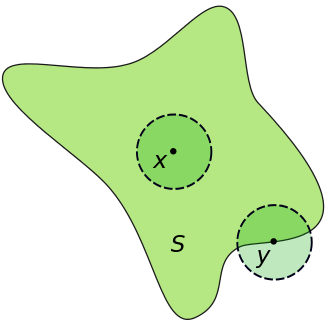
\includegraphics[width=5cm, height=4cm]{images/Interior_illustration.png}
\end{center}

\textcolor{red}{interior有一个性质很重要就是interior是其内部所有点的邻域,所以interior也是一个开集}。

\begin{proof}
假设$M$是$x$的基准开邻域,且$M \subseteq A$,那么$M$里面的所有点都有一个邻域含于$M$,也含于$A$,所以$A$是$M$中所有点的邻域,自然地$M \subseteq A^{\circ}$,所以$A^{\circ}$是$x$的邻域,这里的$x$是任意地。
\end{proof}


\begin{proposition}
集合的内部具有以下基本性质:
\begin{itemize}
	\item $A^{\circ}=A$当且仅当$A$是开集;
	\item $A^{\circ}$是$A$包含的所有开集的并集,也是$A$中最大的开集;
	\item 若$A \subseteq B$,则$A^{\circ} \subseteq B^{\circ}$;
	\item $(A_1 \cap \ldots \cap A_n)^{\circ}=A_1^{\circ} \cap \ldots \cap A_n^{\circ}$;
	\item ${\left(\bigcup\limits_{i \in n} A_i\right)}^{\circ} \supseteq \bigcup\limits_{i \in n} A_i^{\circ}$
\end{itemize}
\end{proposition}
\begin{proof}
\begin{enumerate}
	\item 这个性质根据从邻域出发给出的开集定义很显然。
	\item 如果$A$的子集是一个开集,这个子集很显然也是属于$A^{\circ}$,所以$A$里面的所有开集含于$A^{\circ}$,如何证明$A^{\circ}$是一个开集呢?任取$A^{\circ}$中一点$x$,$A$是$x$的邻域,那么一定存在一个包含$x$的基准开邻域,我们知道基准开邻域是一个并集,根据基准开邻域的定义,这个基准邻域肯定也是属于$A^{\circ}$,由于$x$的任意性,这样的$x$基准开领域都并起来就是$A^{\circ}$,所以$A^{\circ}$是一个开集。再来证明它是$A$内最大的开集,假设如果它不是$A$内最大的开集,那么存在一个更大的开集$A^{'} \supset A^{\circ}$,$A'$是其所有点的邻域(根据开集定义),所有$A' \subseteq A^{\circ}$,这样产生了矛盾,所以$A^{\circ}$是最大的开集。
	\item 根据邻域的最后一条公理,邻域的超集还是邻域,所以B是$A^{\circ}$中所有点的邻域,所以很自然的$A^{\circ} \subseteq B^{\circ}$
	\item 等式的左边表示,所有集合的交的内部,等式的右边表示,所有集合的内部的交,这里为什么等价呢?这个关系用图来说是非常明显的,怎么用文字呢?应该用数学归纳法来证明,我先证明对两个集合是成立的,首先利用第2个性质,${(A_1 \cap A_2)}^{\circ}=U_1 \cup \ldots \cup U_n $,其中$U_1,\ldots,U_n \in A_1 \cap A_2$,很显然它们也属于$A_1^{\circ}$和$A_2^{\circ}$,即${(A_1 \cap A_2)}^{\circ} \subseteq A_1^{\circ} \cap A_2^{\circ}$,反过来$A_1^{\circ} \cap A_2^{\circ}$是一个开集,并且属于$(A_1 \cap A_2)$,所以$A_1^{\circ} \cap A_2^{\circ} \subseteq {(A_1 \cap A_2)}^{\circ}$,两边一夹所以,${(A_1 \cap A_2)}^{\circ} = A_1^{\circ} \cap A_2^{\circ}$,再用一下数学归纳法,即可。
	\item 这个也需要数学归纳法来证明,这里只证明两个集合的情况下,$A_1^{\circ} \cup A_2^{\circ} \subseteq {(A_1 \cup A_2)}^{\circ}$这还是显然的,用第三条性质就可以知道。但是反过来不一样成立,$A_1$和$A_2$的"公共边界"上的点,完全有可能变成$A_1 \cup A_2$内部的点。
	\begin{center}
		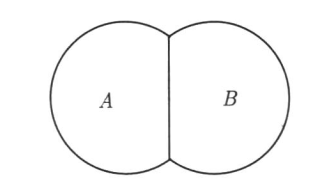
\includegraphics[width=4cm, height=2cm]{images/A_B_same_border.png}
	\end{center}	
\end{enumerate}
\end{proof}

\begin{definition}
如果在拓扑空间$(X,\tau)$中,子集$A$的余集$A^{c}$是开集,则称$A$为\textbf{闭集}(closed set)
\end{definition}

其中余集$A^{c}= X \setminus A$,在平凡拓扑中,闭集就是$\emptyset$和$X$;在离散拓扑中,任何子集都是闭集;闭集和开集互为余集,也可以从闭集出发定义拓扑结构:

\begin{definition}
$X$的子集族$\sigma$是某个拓扑结构下全体闭集构成的集合当且仅当它满足下述三条公理:
\begin{itemize}
	\item $X \in \sigma$,$\emptyset \in \sigma$;
	\item $\sigma$中任意多个元素的交集仍属于$\sigma$;
	\item $\sigma$中任意两个元素的并集仍属于$\sigma$;
\end{itemize}
\end{definition}

我们尝试来推一下开集公理,第一个公理很显然,主要看第二个和第三个,开集和闭集互为余集,如果$A$和$B$为闭集,则$A^c$和$B^c$为开集,根据De Morgan定律\[A^c \cup B^c = (A \cap B)^c , A^c \cap B^c = (A \cup B)^c\],根据闭集公理,上面两个等式结果都是开集。

\begin{definition}
如果$x$每个邻域中都含有$A \setminus \{x\}$中的点,则称$x$为$A$的聚点或者极限点(limit point 或 cluster point 或 point of accumulation),全体聚点构成的集合$A'$称之为$A$的导集(derived set),$\overline{A}=A \cup A'$称为$A$的闭包(closure).换言之,$x \in \overline{A}$当且仅当$x$的每个邻域中都含有$A$中的点。
\end{definition}

聚点的概念对理解闭集有帮助.

\begin{proposition}
拓扑空间$X$中子集$A$闭当且仅当$A$的聚点都含于它本身
\end{proposition}


\begin{proof}
当$A$是闭集,假设存在$A$的聚点$p \in X \setminus A$,$X \setminus A$开且于$A$无交点,与假设矛盾.

当$A$所有聚点含于$A$本身,则$\forall z \in X \setminus A, \exists U_z \cap A = \emptyset$,取遍所有这样的$z$,$X \setminus A=\bigcup\limits_{z \in X \setminus A } U_z$,所以$X \setminus A$,从而$A$是闭集.
\end{proof}

\begin{definition}
设$A$是$X$的一个子集,$A$的边界(\rm boundary)为\[ \partial A:={\bar {A}}\setminus A^{\circ }\].简而言之就是在$A$的闭集但是不在$A$的内部这样的点构成的集合.
\end{definition}

\begin{proposition}
闭包的定义也有几个等价的命题:
	\begin{enumerate}
		\item 所有包含$A$的闭集的交. $\overline A = \bigcap\{C \subseteq X | C \text{ is closed }, A
\subseteq C\}.$
		\item $A$和$A$的边界的交.
	\end{enumerate}
\end{proposition}

\begin{proof}
(1) 这种证明应该经典的两边包含,取任意闭集$C$,使得$A \subseteq C$,假设存在$x \ in X \setminus C$,使得$x \in \overline{A}$,矛盾来了$X \setminus C$开,但是$X \setminus C \cap A = \emptyset$,所以不存在这样的$x$,从而$\overline{A} \subseteq C$. 由于$C$是任意的,所以取交集还是成立\[\overline{A} \subseteq \bigcap C\].

反过来$\overline{A}$本身是闭集(后面一点红色的字),同时它还包含$A$,所以所有包含$A$的闭集的交集肯定是它的一个子集,从而\[\bigcap C \subseteq \overline{A}\].

(2)未来用到boundary的时候,再回过头来证吧...
\end{proof}

%突然多了很多定义,让人触不及防,因为一开始不知道它们的深刻含义。这个定义感觉很模糊,因为没有给$A$到底是什么东西,$x$和$A$关系是什么?

%假设$A$是任意给定一个$X$的子集,那么$x$也是任意取的,所以两者并没有直接关系,而是靠上面刻画的几个关系,首先把用聚点的定义,把$x$和$A$联系起来,然后把这样的$x$都找出来,于是就有全体聚点这个概念,再给它一个定义为导集,把导集和$A$本身并起来,再给一个定义就是闭包。

%上面重新解读了一下定义,那么再研究一下这个闭包有什么性质?闭包$\overline{A}$中任意一点$x$,如果$x \in A'$,则$x$的每个邻域都含有$A$中的点。如果$x \in A$,怎么推出和前面一样的结论呢?注意这样好像只需要含有就行,不需要全含,所以$x$本身在$A$里面这个条件是天然成立的。

\begin{proposition}
设$A$是$X$的一个子集,则$(A^{c})^{\circ}=(\overline{A})^c$.
\end{proposition}

\begin{proof}
这个命题在说明内部和闭包的关系,从右边出发好像简单一点,$A$的闭包的余集,是指那些点$x$的邻域不都包括$A$中的点。换句话说就是指点$x$有一个邻域都只包含$A^c$的点,则这个邻域是含于$A^c$,根据内点的定义,点$x$是$A^c$的内点,所有这样的点,就是$(A^c)^{\circ}$.总结一下就是$A$的闭包和$A^c$的内部互为余集。	
\end{proof}

\textcolor{red}{我们前面已经证明了每个内部都是一个开集,所以闭包是一个闭集}.

于是,所有关于内部的性质都可以用De Morgan定律翻译成闭包的性质

\begin{itemize}
	\item $\overline{A} = A$,当且仅当$A$是闭集。
	\item $\overline{A}$是包含$A$的所有闭集的交集,也是包含$A$的最小闭集。
	\item 若$A \subseteq B$,则$\overline{A} \subseteq \overline{B}$
	\item $(A_1 \cup \ldots \cup A_n)^{\circ}=A_1^{\circ} \cup \ldots \cup A_n^{\circ}$;
	\item ${\left(\bigcap\limits_{i \in n} A_i\right)}^{\circ} \subseteq \bigcap\limits_{i \in n} \overline{A_i}$
\end{itemize}

\begin{proof}
我尝试用$(A^{c})^{\circ}=(\overline{A})^c$,来简单证明一下第一条,若$\overline{A}=A$,则$(\overline{A})^c = A^c=(A^{c})^{\circ}$,后面这个等号根据内部的性质则$A^c$是开集,所以$A$为闭集(开集和闭集互为余集)。
\end{proof}


\begin{definition}
如果$\overline{A}=X$,则称$A$在$X$中稠密(dense)。如果$X$有只含有可数多个元素的稠密子集,则称$X$可分(separable).
\end{definition}

这个定义有点抽象,第一个话是指,定义$X$某个子集$A$,如果对$X$中任意的点$x$,要么属于$A$或者是$A$的一个聚点,则称$A$在$X$中是稠密的。非正式说法是,对于$X$中任意的点$x$,要么属于$A$或者“任意接近”$A$中的某个点。

如何去判定一个子集是不是稠密子集呢? \textcolor{red}{这个是常用的一个判定和构造方法}.
\begin{proposition}
定义拓扑空间$X$下子集$A$,$A$稠密当且仅当对于任意非空开集与$A$的交集非空.
\end{proposition}

\begin{proof}
若$A$稠密子集,其实也就是说$X \setminus A$都是$A$的聚点,所以$X$上任意点的开集都和$A$有交点.

若任意非空开集与$A$都非空,也就是说任意$x \in X$点的开集都与$A$非空,则$X \setminus A$都是$A$上的聚点.
\end{proof}

\begin{example}
有理数集是实数集一个稠密集,因为每一个实数,可能是一个有理数或者存在一个任意接近它的有理数(丢番图近似),严格证明: 假设$\overline{\mathbb{Q}} \neq \mathbb{R}$,则有一点$p \in \overline{\mathbb{Q}} \setminus \mathbb{R}$,$p \notin \mathbb{Q}$,只有可能$q$不是$\mathbb{Q}$的聚点,所以存在一个$q$开区间$(a,b)$与$\mathbb{Q}$没有交点,但根据实数的稠密性$a$和$b$之间是可以确定一个有理数的,这与假设矛盾.
\end{example}

\begin{example}
用$\tau_f$表示$\mathbb{R}$上的余有限拓扑,则$(\mathbb{R},\tau_f)$可分,$\mathbb{N}$就是它的一个可数稠密子集。但是为什么呢?首先$\mathbb{N}$可数,那么为什么$\mathbb{N}$是稠密的呢?根据闭包的性质,$\overline{\mathbb{N}}$等于所有包含$\mathbb{N}$闭集的交集。再根据余有限拓扑的定义,除了$\mathbb{R}$其上闭集是有限的,但是不存在包含$\mathbb{N}$的有限闭集,那包含$\mathbb{N}$的闭集只有$\mathbb{R}$了,所以$\overline{\mathbb{N}}=\mathbb{R}$.
\end{example}

\begin{example}
用$\tau_c$表示$\mathbb{R}$上的余可数拓扑,则$(\mathbb{R},\tau_c)$不可分。任意的$\mathbb{R}$的可数子集$U$,在余可数拓扑上都是闭集,而闭集的闭包是自己,$U \neq \mathbb{R}$,所以不存在这样的可数子集。
\end{example}

下面是一些来自《topology without tears》中的补充性质

\begin{definition}
如果拓扑空间$(x,\tau)$某一个子集$A$,它同时满足开集和闭集,则称它是\textbf{clopen}.
\end{definition}


\newpage
\subsection{Metric Space}

在介绍度量空间之前,还是有必要先讲一下欧式空间,度量空间是欧式空间下的一般情况推广,欧式空间上的拓扑结构怎么表示呢?我先看一维欧式空间$\mathbb{R}$

\begin{definition}
给定$\mathbb{R}$上的子集$S$,若$\forall x \in S$,存在$a \in \mathbb{R}$和$b \in \mathbb{R}$,规定$a < b$,使得$x \in (a,b) \subseteq S$,则$S$是$\mathbb{R}$上标准拓扑中的开集.
\end{definition}

验证上述定义是否满足拓扑结构还是比较简单的,但是这个定义还是比较抽象的,我们也可以更直接一点找出一些开集,例如$R$上的所有形如$(r,s)$,$(-\infty,r)$,$(r,+\infty)$,其中$r,s \in \mathbb{R}$它们是很显然满足欧式拓扑下开集定义的,所以$\mathbb{R}$上的所有\textbf{开区间都是开集},但是反过来就不一定了,因为你可以把两个不相交的开区间并起来.

\begin{proposition}
给定$\mathbb{R}$上的子集$S$,$S$是开集当且仅当$S$是若干开区间的并。
\end{proposition}

很自然地,所有闭区间$[a,b]$都不是开集,因为两端点,并不满足上述定义,但是它们都是闭集,因为你取它的余集$(-\infty,a) \cup (b,+\infty)$是一个开集.还有一些特殊的闭集,例如单点集$\{a\}$和整数集$\mathbb{Z}$.

\begin{proposition}
有理数集$\mathbb{Q}$既不是开集也不是闭集。
\end{proposition}

\begin{proof}
对于任意$q \in \mathbb{Q}$,可以找到两个实数$a$和$b$,使得$q \in (a,b)$,但是这样的$(a,b)$并不属于$\mathbb{Q}$,因为两个实数中间存在无数个实数,并不是有理数,这其中就包括无理数.

为了证明$\mathbb{Q}$同样不是一个闭集,只需要证明$\mathbb{R} \setminus \mathbb{Q}$不是一个开集,取任意的一个开区间$x \in (a,b) \subseteq \mathbb{R} \setminus \mathbb{Q}$,由实数的稠密性,任意两个实数是可以确定一个有理数的,但是$\mathbb{R} \setminus \mathbb{Q}$并不包含有理数,所以不存在这样的开区间,证毕.
\end{proof}

在介绍了$R$上的标准拓扑以后,你可能会想这东西最初是怎么构造出来?其实它可以由某个度量诱导出来,首先我们得了解什么是度量?一个度量就是测量空间中两个点之间距离的一个公式. 当然,为了确保这个公式真的能起到类似距离的作用,它还需要满足一些基本的公理.

\begin{definition}
$X$上的一个度量(metric)是一个映射\[\func{d}{X \times X}{\mathbb{R}}\]满足
\begin{enumerate}
	\item \textbf{正定性}(positive definite) $\forall x,y \in X,d(x,y) \geq 0$,并且$d(x,y)=0$当且仅当$x=y$;
	\item \textbf{对称性}(symmetry) $\forall x,y \in X,d(x,y)=d(y,x)$;
	\item \textbf{三角不等式}(triangle inequality) \[\forall x,y,z \in X,d(x,z) \leq d(x,y)+d(y,z)\].
\end{enumerate}
$X$和$d$合起来叫一个\textbf{度量空间}(metric space),记做$(X,d)$.
\end{definition}

然后呢,在度量空间中可以定义一个自然的基准开邻域结构如下: 考虑那些$B_{\varepsilon}(x)=\Set{y \in X}{d(x,y) < \varepsilon}$.我们称之为$x$的$\varepsilon$-球心邻域($\varepsilon$-ball).取$\mathcal{N}_d(x)=\Set{B_{\varepsilon}(x)}{\varepsilon \> 0}$.

\begin{proposition}
其中$\mathcal{N}_d$确实是$X$上的一个基准开邻域结构.由$\mathcal{N}_d$生成的拓扑$\tau_d$称为度量空间$(X,d)$上的度量拓扑(metric topology).
\end{proposition}

\begin{proof}
需要证明$N_d$满足基准开邻域结构的三条公理:
\begin{enumerate}
	\item $x \in B_\varepsilon(x)$,显然地;
	\item $B_{min(\varepsilon,\delta)}(x)=B_{\varepsilon}(x) \cap B_{\delta}$
	\item 任取$y \in B_{\varepsilon}(x)$,要给它也找一个基准开邻域$B_{\delta}(y)$包含于$B_{\varepsilon}(x)$,那么$B_{\delta}(y)$里面的点也应该是属于$B_{\varepsilon}(x)$,我们不妨再设一点$z \in B_{\delta}(y)$,即$d(y,z) < \delta$,确定合适的$\delta$要求$d(x,z) < \varepsilon$,由三角不等式我们有下面不等式 \[\left\{
		\begin{array}{l}
			d(x,z)\leq d(x,y) + d(y,z) \\ 
			d(y,z) < \delta  \\ 
			d(x,z) < \varepsilon 
		\end{array}
	\right.\]由(1)和(2)可得$d(x,z) < \delta + d(x,y)$,所以我们只需要取$\delta = \varepsilon - d(x,y)$即可.
\end{enumerate}
\end{proof}


\begin{definition}[$\mathbb{R}$上的欧式度量]
$\func{d}{\mathbb{R} \times \mathbb{R}}{\mathbb{R}}$ given by \[d(x,y) = |x-y|, \ \  x,y \in \mathbb{R}.\]
\end{definition}

更一般$\mathbb{R}^n$上的欧式度量表示为$d(x,y) = \sqrt{\sum_{i = 1}^n (x_i-y_i)^2}$.

为了回答前面的标准拓扑和度量空间之间的关系,我们还需定义一下什么是开球.

\begin{definition}
给定度量空间$(X,d)$和一个正实数$r$,取$a \in X$,则以$a$为中心,半径为$r$的开球表示集合$B_r(a)=\Set{x \in X}{d(x,a) < r}.$
\end{definition}


\begin{proposition}
给定度量空间$(X,d)$,$(X,d)$上所有的开球是$X$上某个拓扑$\mathcal{T}$的一组拓扑基. 
\end{proposition}

这里的proof可能要往后翻一下,看一下basis的判定方法. 这个拓扑$\mathcal{T}$就被称为是由度量$d$诱导(induced)出来的拓扑或者topology generated by d. $(X,\tpl)$被称为\textbf{the induced topological space} or \textbf{the corrpesponding topological space} or \textbf{the associated topological space}.


standard topology其实就是由euclidean metric诱导出来的,你可以发现standard topology上的每一个open set都可以由开球覆盖. 而且每一个开球都是standard topology里面的open set, 所以 standard topology generated by euclidean metric. 

反过来也可以说standard topology所在拓扑空间是一个度量空间.
\begin{definition}
设$\tpl_\varepsilon$是$\mathbb{R}^n$上欧式度量所决定的拓扑,则拓扑空间$(\mathbb{R}^n,\tpl_\varepsilon)$为一个$n$维\textbf{欧式空间}(Euclidean space),记为$\mathbb{E}^n$.
\end{definition}


不同的度量作用在同一个集合上可能生成的拓扑结构是相同的.

\begin{definition}
在$X$上的两个度量等价当且仅当它们诱导出的拓扑相同.
\end{definition}


如何判定度量空间上的一个子集是否开(其拓扑是由其度量诱导出来的)?

\begin{proposition}
给定一个度量空间$(X,d)$和由度量$d$诱导出的拓扑$\tpl$,$X$上的子集$U$开当且仅当对任意$x \in U$,存在一个开球$B_\varepsilon(x) \subseteq U$,其中$\varepsilon>0$.
\end{proposition}

\begin{definition}[metrizable]
给定拓扑空间$(X,\tpl)$,若存在$X$上某个度量$d$可以诱导出拓扑$\tpl$,则称$(X,\tpl)$是metrizable.
\end{definition}

\begin{definition}[isometry]
给定两个度量空间$(X,d)$和$(Y,d_1)$,若存在满射$\func{f}{(X,d)}{(Y,d_1)}$,使得对任意的$x_1,x_2 \in X$有\[d(x_1,x_2)=d_1(f(x_1),f_(x_2)).\]则称$f$是一个isometry,$(X,d)$是isometric于$(Y,d_1)$.
\end{definition}

\begin{definition}[Bounded]
给定一个度量空间$(X,d)$,若对任意的$x,y \in X$,存在一个正实数$M$使得$d(x,y) < M$,则称度量空间$(X,d)$是bounded,度量$d$是一个bounded metric.
\end{definition}

\begin{definition}[Bounded Set]
给定度量空间$X$上子集$A$,若存在$y \in X, \varepsilon >0$,使得$A \subseteq B_\varepsilon(y)$,则称$A$有界. 换句话就是$A$能被某个更大的开球盖住.
\end{definition}

上面两张定义都可以相互推的.

\begin{definition}[Totol Boundedness]
给定度量空间$(X,d)$和其上子集$A$,若对任意的$\varepsilon > 0$,都存在一组$x_1,\cdots,x_n \in X$,使得$A \subseteq \bigcup\limits_{i=1}^{n} B_\varepsilon(x_i)$.也就是说$A$可以被有限个半径为$\varepsilon$的开球盖住, 则称$A$ is totally bounded(完全有界).
\end{definition}

可以利用下面的方法去判定度量空间上的闭集.

\begin{proposition}
给定度量空间$(X,d)$,若$X$上的子集$A$是闭的,当且仅当对任意$A$里面的收敛点列都收敛于$A$中一点,换句话说就是$\forall x \in X,a_n \in A$,若$a_n \rightarrow x$,则$x \in A$.
\end{proposition}

\begin{proof}
($\Rightarrow.$)若$A$是一个闭集,假设存在$A$中一个点列$\{a_n\}$收敛于$x \in X \setminus A$. 可以在$X \setminus A$中找到$x$的一个开球$B_\varepsilon(x) \subseteq X \setminus A$,此时对于任意的$a_n$都有$d(a_n,x) > \varepsilon$,这显然是和收敛的定义矛盾的,所以不存在这样的$x$.

($\Leftarrow.$)若$A$中所有收敛点列$\{a_n\}$都收敛于$x \in A$,假设$A$不是一个闭集,我们总可以找到$A$的一个聚点$x \in X \setminus A$(不然$A = \overline{A}$,那么$A$就是一个闭集了). 使得对任意$\varepsilon > 0$,都有$B_\varepsilon(x) \cap A \neq \emptyset$. 现在来构造一个点列$\{a_n\}$,使得这个点列是收敛于$x$. 让$a_n = B_{\frac{1}{n}}(x)$,现在这个点列是收敛于$x$的,因为对应任意的$\varepsilon > 0$,我们取$n_0 > \frac{1}{\varepsilon}$ \[x \in B_{\frac{1}{n}}(x) \subseteq B_{\frac{1}{n_0}}(x) \subseteq B_\varepsilon(x).\]这和前提条件矛盾了,所以不存在这样的$x$.
\end{proof}



\newpage
\subsection{Potency of Set and Countable Set}

对于一个空间来说,比拓扑性质和概念更基本的是它作为集合的那些性质和概念。

\begin{definition}
设$A$,$B$是两个集合。如果存在双射$\func{f}{A}{B}$,则称$A$和$B$的基数(cardinality)或者势(potency)相等,记做$|A|=|B|$.
\end{definition}

\begin{lemma}
如果$A$,$B$是有限集,则$|A|=|B|$当且仅当它们所含的元素相等.
\end{lemma}

\begin{lemma}
如果$A$是无限集,则它必有一个可数无限集
\end{lemma}

\begin{proof}
按顺序每次取一个就行。
\end{proof}

\begin{proposition}
集合$A$无限当且仅当它与一个真子集基数相等.
\end{proposition}

%https://proofwiki.org/wiki/Infinite_Set_is_Equivalent_to_Proper_Subset
\begin{proof}
这个命题值得证明一下,从前面第一个lemma我们知道,如果$A$和真子集基数相等,那它肯定不是有限集。反过来$A$如果不是有限集,则它是无限集,第二lemma可知,我们可以构造一个可数无限集$S=\{a_1,a_2,\ldots\}$,然后对它再分一个类:\[S_1 = \{a_1, a_3, a_5, \ldots\}, S_2 = \{a_2, a_4, a_6, \ldots\}\]再建立一个$S$和$S_1$之间的双射$a_n \leftrightarrow a_{2n-1}$,然后再把这个双射扩展到$S \cup (A \smallsetminus S) = T$ 和 $S_1 \cup (A \smallsetminus S) = A \smallsetminus S_2$,都并上了$A \smallsetminus S$,所以把$a \in A \smallsetminus S$映到它自己就行,还是维持$S$和$S_1$的映射。所以现在建立了一个$A$与$A \smallsetminus S_1$的双射。这个证明看起来就没有那么违反直觉,不错不错。
\end{proof}

\begin{theorem}
Cantor-Schroder-Bernstein,if $|A|\leq|B|$ and $|B|\leq |A|$,then $|A|=|B|$.
\end{theorem}

\begin{proof}
定义两个单射$\func{f}{A}{B}$和$\func{g}{A}{B}$.想象下面的序列:\[\cdots \rightarrow  f^{-1}(g^{-1}(a)) \rightarrow g^{-1}(a) \rightarrow   a  \rightarrow  f(a) \rightarrow  g(f(a)) \rightarrow \cdots\],其中$a \in A$,从$a$点往左好理解,就是重复使用$f$,$g$,那从$a$点往右呢?也很好理解,就是重复使用$f^{-1}$和$g^{-1}$,但是呢它可能到某个位置就停了,因为有可能某个地方它们没有定义了,因为我们只保证了$f$和$g$是一个单射。先理解这个性质,我们再来想办法用$f$和$g$构造一个$\func{h}{A}{B}$的双射.

按照上面的理解,这个序列有三种情况:
\begin{itemize}
	\item 从a点出发转一圈,有转回来了。其实就是指这条路径上的$f^{-1}$和$g^{-1}$都有定义。
	\item 想象一直往左边看,如果某个点$f^{-1}$没有定义,那么其实就在某个$x \in B$位置停下了。
	\item 想象一直往左边看,如果某个点$g^{-1}$没有定义,那么其实就是就在某个$x \in A$位置停下了。	
\end{itemize}

先看后面两种情况,如果在B点停下了,那么我们就让$h(x)$在这点$h^{-1}(x)=g(x)$,即$h(x)=g^{-1}(x)$,现在我们确定了一个点的对应关系,为什么可以这样取呢?因为$g(x)$是单射,确定这点对应的两点之前关系是唯一的,也就是$g(x)$引出的箭头是唯一的(因为$f^{-1})$在这点没有定义了,我们考虑这点的$g^{-1}$。对应的如果在A点停下了,我们就让$h(x)=f(x)$.那么是一个循环序列我们怎么吗?那么对应这个循环序列里面连着的两点,统一用$g^(-1)$或者$f$来表示对应关系,即可。下图,做一个形象记忆,采自wiki。

\begin{center}
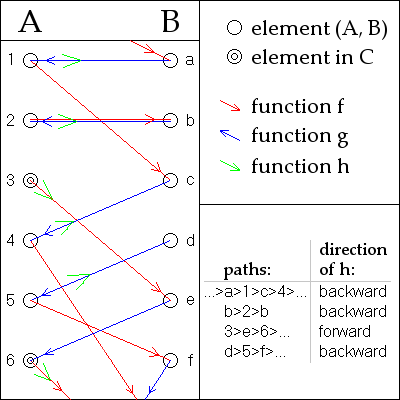
\includegraphics[width=10cm, height=8cm]{images/Cantor-Bernstein.png}
\end{center}

König's definition of a bijection h:A → B from given example injections f:A → B and g:B → A. An element in A and B is denoted by a number and a letter, respectively. The sequence 3 → e → 6 → ... is an A-stopper, leading to the definitions h(3) = f(3) = e, h(6) = f(6), .... The sequence d → 5 → f → ... is a B-stopper, leading to h(5) = g−1(5) = d, .... The sequence ... → a → 1 → c → 4 → ... is doubly infinite, leading to h(1) = g−1(1) = a, h(4) = g−1(4) = c, .... The sequence b → 2 → b is cyclic, leading to h(2) = g−1(2) = b.

\end{proof}


\begin{definition}
若$\|A\| \leqslant \|\mathbb{N}\|$,则称$\|A\|$可数。 
\end{definition}

显然可数集的子集一定也是可数集,并且可数无限集一定和$\mathbb{N}$基数相等。

著名的连续统假设,$\|\mathbb{R}\|$是不是就是紧挨着$\|\mathbb{N}\|=\mathcal{N}_0$的最小基数呢?
\newpage
\subsection{Continuous Map and Homeomorphism}

\begin{definition}
设$X$,$Y$是两个拓扑空间. 如果映射$\func{f}{X}{Y}$满足: 任取$f(x_0)$的邻域$V$,$f^{-1}(V)$都是$x_0$的邻域,则称$f$在$x_0$处\textbf{连续}(continuous). 在定义域上处处都连续的映射称为\textbf{连续映射}(continuous map).
\end{definition}

这个定义要注意的是,连续的条件是“邻域的原像是邻域”,而不是“邻域的像是邻域”,这个地方要想一想,参考函数连续,出发是从$f(a)$的接近程度来找到合适的$x$接近$a$.

\begin{example}
不论$X$,$Y$是什么拓扑空间,取定$b \in Y$,\textbf{常值映射}(constant map)\[\func{e_b}{X}{Y},\ x \mapsto b\]是连续映射,因为$b$的任意邻域的原像都是全空间$X$.
\end{example}

这个逆映射的定义是啥?奇奇怪怪的,直接找原像不就完了吗?:)

\begin{example}
拓扑空间$X$上的\textbf{恒同映射}(identity map)\[\func{id_{X}}{X}{X},\ x\mapsto x\]是连续映射,因为每个邻域的原像都是它本身.注意这里的定义域和值域都是相同的拓扑结构。
\end{example}

\begin{proposition}
对$X$和$Y$分别取定能生成对应结构的基准开邻域结构,则$f$在$x_0$处处连续的充分必要条件是: $f(x_0)$的任何基准开领域$U$的原像$f^{-1}(U)$包含一个$x_0$的基准开邻域.
\end{proposition}

\begin{proof}
基准开邻域也是一个邻域,必要性比较显然,主要看充分性如何证明,$f(x_0)$的任意邻域$U$都有一个基准开邻域$U_0$,即$U \supseteq U_0$,那么$f^{-1}(U) \supseteq f^{-1}(U_0)$,所以$f^{-1}(U)$同样包含一个基准开邻域,即$f$在$x_0$处连续。
\end{proof}

\begin{example}
设$X$,$Y$都是度量拓扑空间,则上述命题说明$\func{f}{X}{Y}$在$x_0 \in X$连续当且仅当$f(x_0)$的任意球形邻域的原像,包含一个$x_0$的球形邻域,这个条件可以进一步改写为:\[\forall \vartheta ,\exists \delta,\text{ 使得 } d_X(x,x_0) < \delta \text{ 蕴含 }d_Y((f(x),f(x_0)) < \vartheta\]
\end{example}

\begin{proposition}
若$\func{f}{X}{Y}$在$x$点连续,$\func{g}{Y}{Z}$在$f(x)$点连续,则$\func{g \circ f}{X}{Z}$在$x$点连续。
\end{proposition}

\begin{proof}
这个命题说明连续的复合还是连续,按照定义来证明,任取$g(f(x))$的邻域$U$,则$g^{-1}(U)$是$f(x)$的邻域,接着$f^{-1}(g^{-1}(U))$是$x$的邻域,因为$(g \circ f)^{-1}(U)=f^{-1}(g^{-1}(U))$,证毕。
\end{proof}

前面用了太多邻域的概念,不妨用本原开集来定义一下连续的概念

\begin{theorem}
考虑一个映射$\func{f}{X}{Y}$,下述两个条件都是$f$为连续映射的充分必要条件:
\begin{enumerate}
	\item $Y$中任意开集关于$f$的完全原像都是$X$中的开集.
	\item $Y$中任意闭集关于$f$的完全原像都是$X$中的闭集.
\end{enumerate}
\end{theorem}

\begin{proof}
从邻域定义的开集出发,先证(1)必要性: 任取$Y$中的开集$U$,对$\forall f(x) \in U$,有$f^{-1}(U)$是$x$的邻域($U$是$f(x)$的邻域,再根据$f$连续),由于$x$是任意的,所以$f^{-1}(U)$是一个开集(根据开集的定义).

再证(1)的充分性: 任取$x \in X$以及$f(x)$的邻域$V$,则存在开集$U$使得$f(x) \subseteq U \subseteq V$,根据命题$f^{-1}(U)$也是一个开集,而$x \in f^{-1}(U) \subseteq f^{-1}(V)$,所以$f^{-1}(V)$是一个邻域.	

(2)的充分必要性,由一个有趣的事实决定: \[f^{-1}(U)^c  = f^{-1}(U^c)\],如果$U^c$是一个开集,那么$f^{-1}(U)$就是一个闭集,同样$U$也是一个闭集。
\end{proof}

\begin{definition}
如果$\func{f}{X}{Y}$是一个双射,并且$f$和$f^{-1}$都连续,则称$f$为\textbf{同胚}(homeomorphism),并且称$X$与$Y$\textbf{同胚}(homeomorphic)或者\textbf{拓扑等价},记为$X \cong Y$.
\end{definition}

同胚的空间具有本质上一样的连续性.仔细想想这个定义可能在刚开始,会有一并且对于每个指标$\lambda in \Lambda$,取定一个拓扑空间$(Y_\lambda,\tpl_\lambda)$以及一个映射$\func{\lambda}{X}{Y_\lambda}$些疑惑,在$\mathbb{R}$上,如果一个$f$是双射,且$f$连续,那为什么还要保证$f^{-1}$连续呢?直觉上前两个条件似乎可以直接保证$f$的逆映射是连续的。

注意这里是连续是拓扑结构上的概念,两个集合之前的一一对应,再确定分别确定两个集合上的拓扑结构之前,啥也保证不了。只有再两个对应的拓扑结构确定以后,我们再来讨论这里的连续到底是什么.举个很显然的例子,说明$f$是双射,$f$是连续的,但是$f$的逆并不连续。

\begin{example}
设$\func{f}{X}{Y}$是一个双射,然后我取$X$上的拓扑结构为离散拓扑,$Y$上的拓扑结构为平凡拓扑。显然在$f$上是连续的,因为不管$f(x)$取什么,其原像对应的子集都是开集,但是反过来$f^{-1}$,就可能不是连续了,因为$Y$上拓扑就两个元素,我大可以找很多$X$上的邻域,对应到$Y$上,并不在这样拓扑里面.
\end{example}

\begin{example}
$\mathbb{R}$任意两个开区间$(a,b)$和$(c,d)$同胚. 把$(a,b)$放到$x$轴上,$(c,d)$放到$y$轴上,$(a,c)$和$(b,d)$那条直线就是$f$. 
\end{example}

\begin{example}
$\mathbb{R}$和开区间$(-1,1)$同胚,构造一个$\func{f}((-1,1))(R)$\[f(x)=\frac{x}{1-|x|}.\]
\end{example}

\begin{example}
更一般地,$\mathbb{R}$和任意的开区间$(a,b)$同胚. 我们直接用上面的$f$来构造.直接移动和放缩定义域就行\[f((\frac{b-a}{2})(x-\frac{(b+a)}{2}))=f((\frac{b-a}{2}x-\frac{b^2-a^2}{4}))=\frac{(\frac{b-a}{2}x-\frac{b^2-a^2}{4})}{1-|(\frac{b-a}{2}x-\frac{b^2-a^2}{4})|}\]
\end{example}

这样看来同胚,其实就是我们在给定一一对应的集合映射上,需要再去关注拓扑结构之间的关系,也就是所谓的连续.

\begin{theorem}
同胚是拓扑空间之间的等价关系.我们称一个关系$\cong$是\textbf{等价关系}(equivalence relation),如果它满足:并且对于每个指标$\lambda \in \Lambda$,取定一个拓扑空间$(Y_\lambda,\tpl_\lambda)$以及一个映射$\func{\lambda}{X}{Y_\lambda}$
\begin{enumerate}
	\item 自反性(reflexivity) $X \cong X$
	\item 对称性(symmetry) 如果$X \cong Y$,则$Y \cong X$ 
	\item 传递性(transitivity) 如果$X \cong Y$,则$Y \cong Z$,则$X \cong Z$
\end{enumerate}
\end{theorem}

\begin{proof}
\begin{enumerate}
	\item 恒同映射$\func{id_X}{X}{X}$.
	\item 同胚的定义.
	\item 前面的提到连续的复合映射,就可以用到这里.
\end{enumerate}
\end{proof}

注意前面的$X$,$Y$,$Z$都表示拓扑空间,就是指对应的各自已经先确定好了拓扑,在这里不要造成歧义。

\begin{definition}
在同胚下保持不变的性质叫拓扑性质(topological property),在同胚下保持不变的概念称为\textbf{拓扑概念}(topological concept),在同胚下保持不变的量称为\textbf{拓扑不变量}(topological invariant).
\end{definition}

对各种类型的拓扑空间进行同胚分类,是拓扑学最基本的研究课题之一。证明两个空间同胚,只要想办法把同胚映射构造出来就行了。而要区分两个空间不同胚,只需要证明一个空间满足某种性质,而另一空间不满足该性质,或者证明对两个空间算某种拓扑不变量的时候,计算结果不同。

\newpage
\subsection{Coarser and Finer}

\begin{definition}
定义集合$X$上的两个拓扑结构$\tpl$和$\tpl'$,我们说$\tpl$比$\tpl'$更弱(coarser or weaker),则$\tpl \subseteq \tpl'$,反过来说就是$\tpl'$比$\tpl$更强(finer or stronger).

换句话说就是,$\tau$比$\tau'$更弱当且仅当在恒同映射下 \[ (X,\tpl') \rightarrow (X,\tpl).\]连续.
\end{definition}


\newpage
\subsection{Product Topology}
这章主要讲如何构造一个拓扑结构?这里有一种非常有趣的定义拓扑结构的方法.设有一个映射$\func{f}{X}{Y}$,集合$X$上尚未确定具体的拓扑结构,而集合$Y$上有个拓扑结构$\tpl'$,则可以利用$f$把这个拓扑"向左转移"到$X$上,即取$\tpl$为$X$上使得$\func{f}{(X,\tpl)}{(Y,\tpl')}$连续的最小拓扑(最小的概念是指最小的$X$的子集族),为什么是最小呢?因为这里$X$可以自然地取离散拓扑做为最大的拓扑.

这个方法可以推广到一族映射$\func{f_\lambda}{X}{Y_\lambda}$上,相应地得到的拓扑就是$X$上所谓的"弱拓扑".类似地,也有一套利用映射"向右转移"拓扑结构的方法,相应地得到的拓扑就是$Y$上的"强拓扑".弱拓扑和强拓扑作用,都是利用映射把一个空间上的拓扑结构以最能充分利用该映射的方式转移到另一个空间上去.

弱拓扑和强拓扑的观点主要是让我们理解这些拓扑"为什么这样定义".


\begin{definition}
考虑一个集合$X$.设$\Lambda$是一个指标集,并且对于每个指标$\lambda \in \Lambda$,取定一个拓扑空间$(Y_\lambda,\tpl_\lambda)$以及一个映射$\func{f_\lambda}{X}{Y_\lambda}$.则$X$上满足条件每个$\func{\lambda}{X}{Y_\lambda}$都连续的最小拓扑$\tpl$称为由这些$f_\lambda$决定的\textbf{弱拓扑}(weak topology).
\end{definition}

注意前面已经提到过的最小的含义,如果更形式化的理解是:如果有其他拓扑$\tpl_0$也满足上述条件,则$\tpl \subseteq \tpl_0$.

那么如何构造这个弱拓扑呢?上述条件也可以理解为要求每个$Y_\lambda$中开集的原像都是开集,所以$\tpl$是包含这些原像的,但是只包含这些原像是不够的,因为我们并不能保证这些原像的交或者并是满足开集公理的,解决办法是把这些原像先取有限交$\bigcap\limits_{\text{finite}} U$,在任意的并起来$\bigcup\limits_{\text{infinite}} \left( \bigcap\limits_{\text{finite}} U \right)$.

我真想把这些穿插的基准开邻域去掉,把subbasis弄上去!!!!

\begin{proposition}
设$\Lambda$是一个指标集,并且对于每个指标$\lambda \in \Lambda$,取定一个拓扑空间$(Y_\lambda,\tpl_\lambda)$以及一个映射$\func{f_\lambda}{X}{Y_\lambda}$.取 \[\mathcal{U}(x)=\Set{f_{\lambda}^{-1}(U_\lambda)}{\lambda \in \Lambda,f_\lambda(x) \in U_\lambda \in \tpl_\lambda}\],然后取\[\mathcal{N}(x)=\{\mathcal{U}(x)\text{ 中有限个元素的交集}\}\],这样得到的$\mathcal{N}$是一个subbasis。并且由它生产的拓扑就是$X$上由这些$f_\lambda$决定的弱拓扑
\end{proposition}

\begin{proof}
subbasis生成拓扑过程是很自然的,然后我们来说明它是最小的拓扑,只需要证明它是含于$X$上的任意拓扑,假设任意$X$上的拓扑$\tpl$,取$U_\lambda \in \tpl_\lambda$,则$f^{-1}(U_\lambda) \in \tpl$,因此$\mathcal{N}(x)$含于$\tpl$,而由$\mathcal{N}$生成的拓扑中的开集都是其中任意元素的并,所以也是属于$\tpl$,这说明$\mathcal{N}$生成的拓扑是$\tpl$的子族.
\end{proof}

生成弱拓扑的过程简而言之就是\[\{U_\lambda\}\stackrel{\cap_{finite}}\longrightarrow \mathcal{N}\stackrel{\cup_{arbitrary}}\longrightarrow \tpl\], generate by subbasis.


\begin{example}
设$(Y,\mu)$是一个拓扑空间,$X$是一个集合,考虑$X$到$Y$的所有映射构成的结合$Y^X$.任取$x \in X$可以定义赋值函数\[\func{e_x}{Y^{X}}{Y}, e_x(f)=f(x).\]于是$Y^{X}$上就有一个由所有这些$e_x$决定的弱拓扑.这种弱拓扑刻画的映射空间的“连续性”,是数学分析里面函数序列的"逐点收敛"概念的拓扑推广。
\end{example}

有了弱拓扑的概念,我们可以尝试去理解一下乘积拓扑“为什么它要这么构造”。


\begin{definition}
设$(X,\tpl_X)$,$(Y,\tpl_Y)$是两个拓扑空间.令\[\tpl = \Set{\bigcup\limits_{\lambda \in \Lambda}(U_\lambda \times V_\lambda)}{\forall U_\lambda \in \tpl_X, \forall V_\lambda \in \tpl_Y},\]则$\tpl$是$X \times Y$上的一个拓扑结构,称为$\tpl_X$和$\tpl_Y$的\textbf{乘积拓扑}(product topology).拓扑空间$(X \times Y,\tpl)$称为这两个空间的\textbf{乘积空间}(product space),记为$(X,\tpl_X) \times (Y,\tpl_Y)$.
\end{definition}

%简而言之,$X \times Y$中的子集开当且仅当它是形如$(U \times V)$的子集的并集,这里要求$U$,$V$分别是$X$和$Y$上开集,但是为什么要这样定义?

这里的乘号定义如下:

\begin{proposition}
设$(X,\tpl_X)$,$(Y,\tpl_Y)$是两个拓扑空间.考虑集合$X$和$Y$的直积$X \times Y=\Set{(x,y)}{x \in X,y \in Y}$,在其上定义\textbf{投影}(canonical  projection)\[\begin{aligned}
			\func{j_X}{X \times Y}{X} ,& (x,y) \mapsto x;\\
			\func{j_Y}{X \times Y}{Y} ,& (x,y) \mapsto y; 
			\end{aligned}
			\]则$X \times Y$上由$j_X$,$j_Y$决定的弱拓扑就是乘积拓扑.		
\end{proposition}

有点小疑问,这里的一组映射值域和前面提到的似乎有点不同啊?弱拓扑并没有要求映射的值域是相同的,定义域是相同的即可.

\begin{proof}
分别取$X$和$Y$的开集$U$和$V$,注意到$j_X^{-1}(U) \cap j_Y^{-1}(V)=(U \times V)$,并且\[(U_1 \times V_1) \cap (U_2 \times V_1)=(U_1 \cap U_1)\times (V_1 \cap V_2).\]后面性质为了进一步保证我们先交再做preimage或者先preimage再交都是没有任何问题的. subbasis可以简单表示为\[\mathcal{N}(x)=\Set{(p_x,p_y)}{p_x \in U \in \tpl_X,p_y \in V \in \tpl_Y}.\]
\end{proof}

$j_X^{-1}(U) \cap j_Y^{-1}(V)=(U \times V)$可以很形象的用一个方形邻域来描述.

\begin{center}
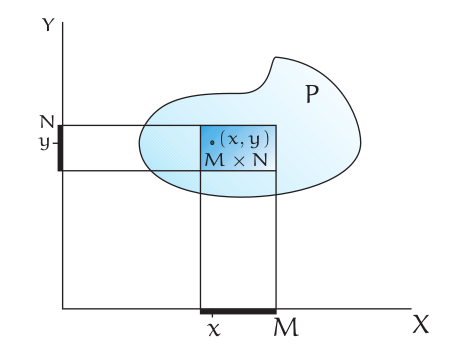
\includegraphics[width=10cm, height=8cm]{images/product_topology.png}
\end{center}

\begin{definition}
乘积拓扑的万有性质是指存在一些连续映射$\func{f_\alpha}{Z}{Y_\alpha}$,则存在唯一的连续映射$\func{g}{Z}{\prod Y_\alpha}$,其中$q_\alpha \circ \ g = f_\alpha$.
\begin{center}
% https://tikzcd.yichuanshen.de/#N4Igdg9gJgpgziAXAbVABwnAlgFyxMJZABgBpiBdUkANwEMAbAVxiRAC0QBfU9TXfIRQAmclVqMWbADrS0AJ2gACAJoB9WYzQALOt14gM2PASKjh4+s1aIQ6zQx16u4mFADm8IqABmigLZIZCA4EEgAjNRWUrbu+r4BEdShSKIS1mwAjhrSWrrxIH4QgYjBKYhp0TaFOXnOFFxAA
\begin{tikzcd}
Z \arrow[rr, "g"] \arrow[rrdd, "f_\alpha"] &  & \prod Y_\alpha \arrow[dd, "q_\alpha"] \\
                                           &  &                                       \\
                                           &  & Y_\alpha                             
\end{tikzcd}
\end{center}
注意$\prod Y_\alpha$表示无穷乘积.
\end{definition}


\begin{example}
设$(X,d_X)$,$(Y,d_Y)$是两个度量空间,则在$X \times Y$上可以定义度量$d$如下: 任取两点$p=(p_x,p_y)$,$q=(q_x,q_y)$,\[d(p,q)=max(d_X(p_x,q_x),d_Y(p_y,q_y))\]并且该度量决定的度量拓扑就是$X \times Y$上的乘积拓扑.
\end{example}

在证明上述命题之前,我们可以简单思考一下$d$确实是一个度量,有趣的为什么不能把$max$换成$min$?
%why max not min https://pages.uoregon.edu/adding/courses/431-18/midterm1_sol.pdf

%让$x \in X$,$y \in Y$,我们希望定义一个$(x,y)$的邻域,直觉上邻域里面的点$(x',y')$要尽可能的接近$(x,y)$,那么应该是$x$和$x'$接近,$y$和$y'$接近,这种想法不就是分别去取$x$在$X$和$y$在$Y$里面的邻域吗?但是呢,这样定义出来的$X \times Y$邻域是有问题的,观察上面的图,$M$和$N$分别是$X$和$Y$中$x$和$y$的邻域,按照邻域公理如果一个集合$P$包含$M \times N$,那么$P$也应该是一个邻域,现在你会发现这个形状不规则的$P$,你似乎没办法用$X$和$Y$里面的邻域表示了.

\begin{proof}
先写一下我们的证明思路,要证明上述度量诱导出来的拓扑是乘积拓扑:(1)在乘积拓扑中找邻域,这个邻域在$d$度量诱导的拓扑里面(2)在$d$度量诱导的拓扑里面找邻域,这个邻域在乘积拓扑里面.

(1)在乘积拓扑下,如果一个子集$A \subseteq X \times Y$是$p(p_x,p_y)$邻域,那么存在一个开集含于它,所以我们必须找到这样一个$X \times Y$乘积拓扑里面的开集,乘积拓扑上的开集为$\bigcup(U,V)$,其中$U \in \tpl_X$,$V \in \tpl_Y$.这样不好操作啊,怎么把前面个bigcup去掉呢?其实可以比较从容的去掉,因为点$p$肯定属于某个$X$开集,开集自包含,同样是$p$的一个邻域.那么我们的命题可以变成下面的样子:

$A$是邻域的充分必要条件是: 分别存在$X$中的开集$U$和$Y$中的开集$V$,使得$p \in U \times V \subseteq A$.如果我们能找到这样的$U$,$V$,进一步我们可以分别找到它们里面分别关于$p_x$的邻域$B_\zeta(p_x)$和$p_y$的邻域$B_\delta(p_y)$。然后我们知道\[B_{min(\zeta,\delta)}(p) \subseteq B_\zeta(p_x) \times B_\delta(p_y)\]其中$B_{min(\zeta,\delta)}(p)$就是一个$d$度量下的邻域,$A$包含它,所以$A$也是$d$度量诱导的拓扑下的邻域.

(2)在$d$度量诱导的拓扑下,任意的$A$邻域包含一个$p=(p_x,p_y)$的一个邻域$B_\varepsilon(p)$,而\[B_\varepsilon(p)=B_\varepsilon(p_x) \times B_\varepsilon(p_y)\],其中$B_\varepsilon(p_x)$和$B_\varepsilon(p_y)$分别是$X$和$Y$下的邻域,各自在找一个开集,所以$A$也是乘积拓扑下的邻域.
\end{proof}


\begin{definition}
对于一个映射$\func{f}{A}{X \times Y}$,设\[f_X = j_X \circ f, \quad f_Y = j_Y \circ f,\]换言之$f(a) \equiv (f_X(a),f_Y(a))$,则称$f_X$,$f_Y$为$f$的分量(component).
\end{definition}

\begin{theorem}
映射$\func{f}{A}{X \times Y}$连续的充分必要条件是两个分量$f_X$和$f_Y$都连续.
\begin{center}
% https://tikzcd.yichuanshen.de/#N4Igdg9gJgpgziAXAbVABwnAlgFyxMJZABgBoBGAXVJADcBDAGwFcYkQAtEAX1PU1z5CKAEwVqdJq3YBNAPrkABAB1leALbxF8kTz4gM2PASIAWUsQkMWbRCHnk9-I0LOkRVqbftzd3CTBQAObwRKAAZgBOEOpIZCA4EEjkNNbSduFOIFExyTSJSGKSNuxoClk5sYgpCUmIAMw0jPQARjCMAAoCxsIgkVhBABY4IKlepb48lNxAA
\begin{tikzcd}
                  &  &                                                       &  & Y_1 \\
Z \arrow[rr, "f"] &  & Y_1 \times Y_2 \arrow[rru, "p_1"] \arrow[rrd, "p_2"'] &  &     \\
                  &  &                                                       &  & Y_2
\end{tikzcd}
\end{center}
\end{theorem}

\begin{proof}
如果$f$连续,由复合映射的连续性可知,$f_X$和$f_Y$也都连续.反过来如果$f_X$和$f_Y$都连续,$f^{-1}(U \times V)=f_X^{-1}(U) \cap f_Y^{-1}(V)$,开集的交还是开集,所以$f$连续.
\end{proof}

\begin{example}
考察平面上的一条参数曲线$x(t)=(x_1(t),x_2(t))$.上面定理告诉我们,$x$连续当且仅当$x_1$,$x_2$都连续.
\end{example}

乘积拓扑?弱拓扑?奇妙... 再来感受一下乘积拓扑里面一些有趣的性质

\begin{proposition}
让$C_1,C_2,\cdots,C_n$分别表示拓扑空间$X_1,X_2,\cdots,X_n$上的闭集,则$C_1 \times C_2 \times \cdots \times C_n$是乘积空间$X_1 \times X_2 \times \cdots \times X_n$上的闭集.
\end{proposition}

\begin{proof}
$(X_1 \times X_2 \times \cdots \times X_n) \setminus C_1 \times C_2 \times \cdots \times C_n = [(X_1\setminus C_1) \times X_2 \times \cdots \times X_n] \cup [X_1 \times (X_2\setminus C_2) \times \cdots \times X_n] \cup \cdots \cup [X_1 \times X_2 \times \cdots \times (X_n\setminus C_n).]$ 
\end{proof}


\newpage
\subsection{Subspace Topology}

拓扑空间$X$的一个子集$A$上可以很简单地定义一种非常自然的拓扑结构,称为子空间拓扑.子空间拓扑也是使得含入映射$i \colon A \hookrightarrow X$连续的最弱拓扑.

\begin{definition}
设$(X,\tpl)$是个拓扑空间,$A \subseteq X$,令\[\tpl|_A=\Set{U \cap A}{U \in \tpl}\],则$\tpl|_A$是$A$上的一个拓扑,称为$A$上的\textbf{子空间拓扑}(subspace topology),而拓扑空间$(A,\tpl|_A)$称为$(X,\tpl)$的子空间(subspace).
\end{definition}

\begin{proposition}
设$A$是拓扑空间$(X,\tpl)$上的子集,$\func{i}{A}{X}$是一个含入映射,则$A$上由$i$决定的弱拓扑就是子空间拓扑.
\end{proposition}

\begin{proof}
这个命题还是比较显然的,因为$i^{-1}(U)=U \cap A$.
\end{proof}

注意区分子空间上开集并不直接等价于原拓扑空间上的开集.

\begin{lemma}
设$A$是$X$的子空间,如果$U$是$A$上的开集,同时$A$也是$X$上的开集,则$U$也是$X$上的开集.
\end{lemma}


还有下面几个比较简单的性质:

\begin{proposition}
\begin{enumerate}
	\item 如果$B \subseteq A \subseteq X$,则$\tpl|_B = (\tpl|_A)|_B.$
	\item $U$是$(A,\tpl|_A)$里的开集当且仅当存在$(X,\tpl)$中的开集$V$使得$U = V \cap A.$
	\item $U$是$(A,\tpl|_A)$里的闭集当且仅当存在$(X,\tpl)$中的闭集$V$使得$U = V \cap A.$
\end{enumerate}
\end{proposition}

这里需要非常注意一个东西,无论是开集还是闭集,一定要讲清楚是相对哪个拓扑而言的,这一点非常重要.

\begin{definition}
子空间上的万有性质是指对于任意的连续映射$\func{g}{Z}{Y}$,如果$g(Z) \subseteq X$,其中$X$表示$Y$的一个子空间,则存在唯一的连续映射$\func{f}{Z}{X}$.

\begin{center}
% https://tikzcd.yichuanshen.de/#N4Igdg9gJgpgziAXAbVABwnAlgFyxMJZABgBoBGAXVJADcBDAGwFcYkQAtEAX1PU1z5CKAEyli1Ok1bsAmjz4gM2PASJiRkhizaIQADR6SYUAObwioAGYAnCAFskZEDghJyNbTL2mF1u46Izq5IYlI67FZ+ILYO7jQhiGFeuiBYAHrAALTk3EbcQA
\begin{tikzcd}
                                    &  & Y \arrow[dd, "i^{-1}"] \\
Z \arrow[rru, "g"] \arrow[rrd, "f"] &  &                        \\
                                    &  & X                     
\end{tikzcd}
\end{center}
\end{definition}


\begin{example}
定义$\mathbb{Z}$表示$\mathbb{R}$欧式拓扑空间上的包含所有整数的子空间,则$\mathbb{Z}$是一个离散拓扑. 这个还是比较显然,只要说明$\mathbb{Z}$上所有的单点集都是开集就行,任取一个整数$n$,你都可以找到一个$\mathbb{R}$上开区间$(n-1,n+1)$包含只包含它.
\end{example}


\begin{example}
我们来思考一个度量空间上的自然的子空间是什么呢?设$(X,d)$是一个度量空间,度量拓扑为$\tpl$.$A$是$X$的子集,则可以在$A$上规定一个自然的度量$d_A$,使得任取$x,y \in A$,$d_A(x,y)=d(x,y)$.任取$a \in A$,考察它在$X$中的一个$\varepsilon$球型邻域$B_\varepsilon=\Set{x \in X}{d(a,x) < \varepsilon}$,你会发现\[B_\varepsilon \cap A = \Set{x \in A}{d(x,y) < \varepsilon}.\]恰好就是$a$在$A$中关于度量$d_A$的$\varepsilon$球形邻域.	
\end{example}


\begin{example}
设$X$和$Y$是两个拓扑空间,$A$是$X$的子空间.此时可以考虑一个映射$\func{f}{X}{Y}$在$A$上的\textbf{限制映射}(restriction map)\[\func{f|_A}{A}{Y},\ x \mapsto f(x).\]
\end{example}

\begin{lemma}
\textbf{粘接引理}(pasting lemma) 设$\{C_1,\ldots,C_n\}$是$X$的一个\textbf{有限覆盖}(finite closed cover),即由有限多个$X$的闭子集构成的子集族,满足$C_1 \cup \ldots \cup C_n=X$.如果映射$\func{f}{X}{Y}$使得每个$f|_{C_k}$都连续,则$f$连续.
\end{lemma}

\begin{proof}
任取$Y$中的闭集$A$,\[\begin{aligned} 
					f^{-1}(A)&=f^{-1}(A) \cap (C_1 \cup \ldots \cup C_n)\\
					&=(f^{-1}(A) \cap C_1) \cup \ldots \cup (f^{-1}(A) \cap C_n).\end{aligned}\]第一行是简单的变换,整理成子空间拓扑形式,其实就是$A$在$f|_{C_k}$的原像,因为每个$f|_{C_k}$都连续,所以按照定义${f|_{C_k}}^{-1}(A)=D_K \cap C_k = f^{-1}({A}) \cap C_K $在$C_k$中也是闭的,其中$D_k$也是某个闭集,然和有限多个闭集并还是闭集,即$f^{-1}(A)$是闭集.
\end{proof}

\begin{definition}
设$\func{f}{X}{Y}$是连续单射,在$f(X) \subseteq Y$取子空间拓扑,然后考虑映射\[\func{g}{X}{f(X)},\ x \mapsto f(x).\]如果$g$是同胚,则称$f$为\textbf{嵌入}(embedding).
\end{definition}

嵌入是同胚的推广.含入映射就是嵌入的典型例子.


\newpage
\subsection{Quotient Map and Quotient Space}
和弱拓扑相对应地,有另外一种非常自然的定义拓扑结构的方法叫“强拓扑”,就是利用映射$\func{f}{X}{Y}$把集合$X$上的拓扑结构$\tpl$“向右转移”到集合$Y$上去.那么这里为什么叫强拓扑呢?因为使得$f$连续的$Y$上的最小拓扑是平凡拓扑$\{Y,\emptyset\}$,现在要取使得$f$连续的$Y$上最强的拓扑(即在对于集合族中是最大的).


\begin{definition}
设有一族拓扑空间$(X_\lambda,\tpl_\lambda)$及映射$\func{f_\lambda}{X_\lambda}{Y}$.则$Y$上满足条件使得每个$f_\lambda$都连续的最大拓扑$\tpl$称为由这些$f_\lambda$决定的强拓扑(strong topology).
\end{definition}

最大的意思是: 如果有其他拓扑$\mu$也满足上述条件,则$\tpl \supseteq \mu$.那么如何构造最强拓扑?

\begin{definition}
设有一族拓扑空间$(X_\lambda,\tpl_\lambda)$及映射$\func{f_\lambda}{X_\lambda}{Y}$.则$Y$上使得所有$f_\lambda$都连续的最强拓扑为\[\tpl = \Set{U \subseteq Y}{\forall f_\lambda^{-1}(U) \in \tpl_\lambda}\].
\end{definition}

上面的命题就说把$Y$里面在所有$f_\lambda$下原像都是开集的子集搞到一块就是最强拓扑.

\begin{proof}
现在来证明这个$\tpl$确实是个拓扑结构,很明显$\emptyset \in \tpl$和$X \in \tpl$.有\[f^{-1}_\lambda(\bigcup\limits_{\alpha} U_\alpha)=\bigcup\limits_\alpha f_\lambda^{-1}(U_\alpha).\]所以当$U_\alpha \in \tpl$,则$f^{-1}_\lambda(\bigcup\limits_{\alpha} U_\alpha) \in \tpl$.同理,有\[f^{-1}_\lambda(\bigcap\limits_{\alpha} U_\alpha)=\bigcap\limits_\alpha f_\lambda^{-1}(U_\alpha).\]所以当$U_\alpha \in \tpl$,则$f^{-1}_\lambda(\bigcap\limits_{\alpha} U_\alpha) \in \tpl$.然后再说明这个拓扑是最强的,取满足上述条件任意拓扑$\mu$,任取$U \in \mu$,则每个$f_\lambda^{-1}(U) \in \tpl_\lambda$,所以$U \in \tpl$,由于$U$是任意的,所以$\mu \subseteq \tpl$.
\end{proof}

\begin{definition}
设$(X,\tpl_X)$,$(Y,\tpl_Y)$是两个拓扑空间,$\func{f}{X}{Y}$是一个满射,并且$\tpl_Y$恰好是$f$所决定的强拓扑,即$U \subseteq Y$是开集当且仅当$f^{-1}(U) \subseteq \tpl_X$,则称$f$为商映射(quotient map).
\end{definition}

注意在这里区分开映射,开映射肯定是一个商拓扑,但是商拓扑并不一定是一个开映射.在给定单个$f$下,把所有$U \subseteq Y$的原像是开的这样的子集$U$都拿过来当开集,形象地描述"最大拓扑",也可以说是"最细拓扑",这个拿法确实能构造一个拓扑前面已经证明了.

下面是另一定义商映射的方法:
\begin{proposition}
设$\func{f}{X}{Y}$是一个满射,则$f$是商映射的充分必要条件是: $U$是开集(闭集)当且仅当$f^{-1}(U)$是开集(闭集).
\end{proposition}

\begin{proposition}[the universal property of quotient maps]
给定一个商映射$\func{p}{X}{Y}$,则对任意使得$\forall x,x' \in X$,当$p(x)=p(x')$有$g(x)=g(x')$的连续映射$\func{g}{X}{Z}$,存在唯一连续映射$\func{h}{Y}{Z}$使得$h \circ p =g$.
\begin{center}
% https://tikzcd.yichuanshen.de/#N4Igdg9gJgpgziAXAbVABwnAlgFyxMJZABgBpiBdUkANwEMAbAVxiRAA0QBfU9TXfIRQAmclVqMWbAFrdeIDNjwEiARlKrx9Zq0QgAmt3EwoAc3hFQAMwBOEALZIyIHBCTqJOtqbnW7jxGdXJFEQBjoAIxgGAAV+ZSEQGyxTAAscEGptKT00XxBbBxDqYMQPcKjY+ME2ZLSMrMldEFSjLiA
\begin{tikzcd}
X \arrow[rr, "g"] \arrow[rd, "p"'] &                    & Z \\
                                   & Y \arrow[ru, "h"'] &  
\end{tikzcd}
\end{center}
\end{proposition}

\begin{proof}
首先我们得知道上述命题中的条件在刻画什么东西?
\begin{center}
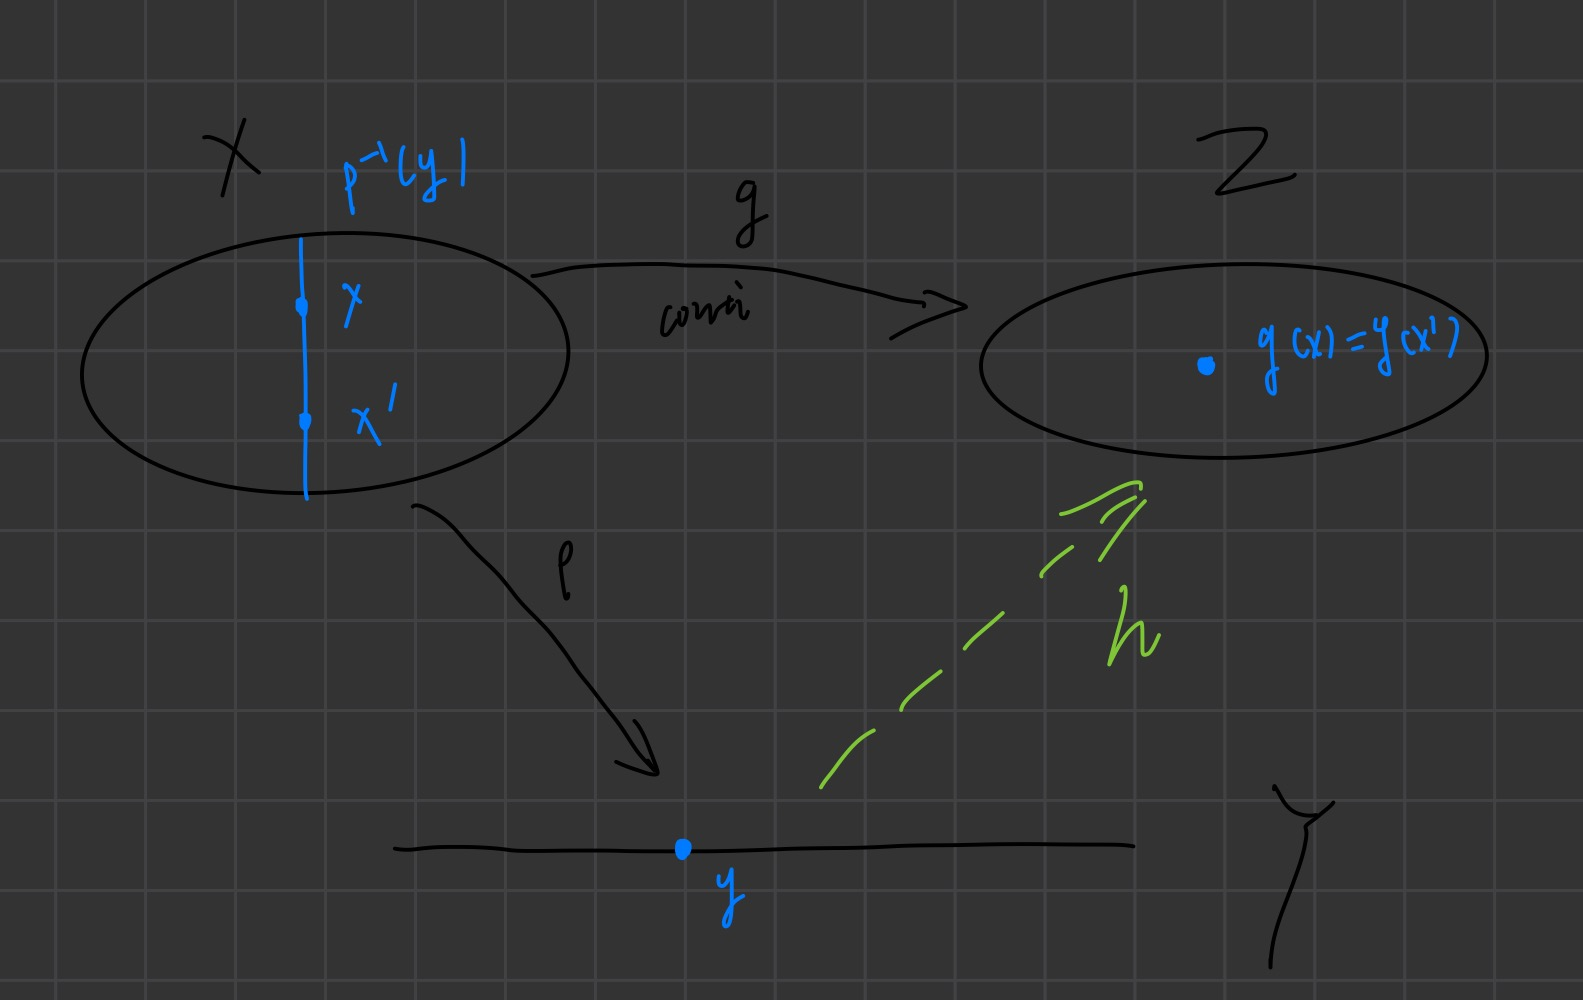
\includegraphics[width=10cm, height=8cm]{images/universal_property_of_quotient_map.JPG}
\end{center}
上面的条件换句话说就是$g$在$p^{-1}(y)$(对任意的$y \in Y$)上是一个constant map,很显然在$p$是一个满射且满足上述条件的情况下,这个映射$h$是唯一存在的即$h(y)=h(p(x))=g(x)$,对任意$x \in p^{-1}(y)$. 我们可以来检验一下$h$是不是well-defined,也就是说它不会随着$x$的选择而改变. 对于每一个$y \in Y$, 我们有$\forall x,x' \in p^{-1}(y),\ p(x)=p(x')$,所以$g(x)=g(x')$,即$h(y)=g(x)$是唯一的. 在$y = y'$时,我们有$p^{-1}(y) = p^{-1}(y')$,所以对于$x \in p^{-1}(y),x' \in p^{-1}(y')$,也有$p(x)=p(x')$,即$g(x)=g(x')$,对于单个$y$原像有相同的函数值这很显然的,所以整体上$h(y)=h(y')$.

再来看$h$为什么连续,则任取$Z$里面的开集$U$,因为$p$是商映射,所以想要看$h^{-1}(U)$是不是开的,就是要看$p^{-1}(h^{-1}{U})$是不是开的,有$p^{-1}(h^{-1}{U}) = g^{-1}(U)$,因为$g$是一个连续映射,所以$p^{-1}(h^{-1}{U})$是开的,所以$h^{-1}(U)$也是开的,即$h$是一个连续映射.
\end{proof}


\begin{proposition}
两个商映射的复合映射还是商映射.
\end{proposition}


下面这个性质会经常的用到.

\begin{proposition}
设$\func{f}{X}{Y}$是个连续满射,则下列两个条件都是$f$是商映射的充分非必要条件:
\begin{enumerate}
	\item $f$是开映射(open map),即任意开集$A \subseteq X$在$f$下的像集是$Y$中的开集.
	\item $f$是闭映射(closed map),即任意闭集$A \subseteq X$在$f$下的像集是$Y$中的闭集.
\end{enumerate}
\end{proposition}

\begin{proof}
当$f$是一个满射时,$U=f(f^{-1}(U))$,其中$U \in Y$,在开映射的条件下若$f^{-1}(U)$是一个开集,那么$U$也是一个开集,同时$f$连续,所以$U$开,那么$f^{-1}(U)$开,证毕。为什么这是充分条件呢?因为商映射的定义是我们在$Y$里面挑子集,如果它的原像是开集,就把它放到$\tpl_Y$里面,当我们挑完$Y$所有子集的时候,可能也只对应了一部分$X$中的开集,现在如果要求$X$所有开集都映射到$Y$上,毫无疑问这时候我们只需要把$X$上的开集的像放到$\tpl_Y$就行了,这个过程就完全确定了.
\end{proof}

显然同胚是一个商映射。那么如何形象的理解商映射呢?在代数里面有商群和商环,但是它们都有一个比较特殊的性质就是构造了很多的等价类,相当于把两个在某种等价关系的刻画下放到了一个等价类里面,在拓扑上的商映射不仅仅是一个满射(满射描述是元素到等价类的映射),还需要附加连续的存在. 商映射带来了一种“拓扑粘合”的观点: 我们可以把被$f$映射到同一个像上的$X$中的点理解成是被粘在了一起,然后把$f(X)$整体理解称是用$f$把$X$粘起来的空间. 

生活中我们可以用一些小纸片涂上胶水粘出复杂的手工艺品,或者把积木插在一起搭出复杂的大模型.商映射就是拓扑空间的胶水,它让我们可以去刻画以前无法想象的复杂空间,把它们分解成简单直观的小块,并为分解和重新组装等操作提供严禁可靠的拓扑解释.

这种理解很是奇妙,需要靠例子来细细品尝...

\begin{theorem}
设$\func{p}{X}{Y}$是商映射,则任取映射$\func{f}{Y}{Z}$,$f$连续当且仅当$\func{f \circ p}{X}{Z}$连续.
\end{theorem}

\begin{proof}
若$f$连续,任取$U \in Z$,其中$U$是开集,所以$f^{-1}(U)$是开集,$p$是商映射,那么$p^{-1}(f^{-1}(U))$也是开集,所以$f \circ p$连续.若$f \circ p$连续,还是任取$Z$中的开集的$U$,则$p^{-1}(f^{-1}(U))$是开集,$p$是商映射,所以$f^{-1}(U)$是$Y$中的开集,所以$f$连续.
\end{proof}

\begin{theorem}
如果$\func{p}{X}{Y}$和$\func{q}{X}{Z}$都是商映射,并且$p(x)=p(x')$当且仅当$q(x)=q(x')$,则$Y$和$Z$同胚.
\begin{center}
% https://tikzcd.yichuanshen.de/#N4Igdg9gJgpgziAXAbVABwnAlgFyxMJZARgBoAGAXVJADcBDAGwFcYkQANEAX1PU1z5CKcqWLU6TVuwCaPPiAzY8BIgCYxEhizaIQALR4SYUAObwioAGYAnCAFskokDghIyIRvQBGMRgAUBFWEQGyxTAAscEBptaT00eWs7R0RnVyQNSR12AEckkFsHdxoMxCy43UKjbiA
\begin{tikzcd}
                  & X \arrow[ld, "p"'] \arrow[rd, "q"] &   \\
Y \arrow[rr, "f"] &                                    & Z
\end{tikzcd}
\end{center}
\end{theorem}

\begin{proof}
终于有一点范畴的东西了,这里要说明$Y$和$Z$同胚,需要先构造$Y$和$Z$之间的映射$f$,上述命题已经给出了一个非常显然的命题,$p$和$q$给出的等价类是一一对应的,那我们定义这样一种映射$\func{f}{Y}{Z}$,即$Y$中任意元素对应于$p(x)$,$f$把它映到$q(x)$,任取$Z$中开集$U$,其中$q(x) \in U$对应$p(x) \in f^{-1}(U)$,,$f$是双射,有"并且$p(x)=p(x')$当且仅当$q(x)=q(x')$"保证,即它们的原像$A$是一样的,因为$q$是商映射,所以$A$是$X$中的开集,作用到同样是商映射的$p$上,我们就可以得到一个$Y$上的开集$p(A)$,同理再证一下$f^{-1}$,这样$f$下的$Y$和$Z$是同胚的。
\end{proof}

\begin{definition}
称$\mathbb{E}^3$中过原点的直线为中心直线.所有中心直线构成的拓扑空间\[\mathbb{R}\mathbb{P}^2=\{\mathbb{E}^3\text{里的中心直线}\}\]称为实射影平面,简称射影平面,其上的拓扑定义为如下度量所决定的度量拓扑: 任取两条中心直线$\mathcal{l}_1$, $\mathcal{l}_2$,$d(\mathcal{l}_1,\mathcal{l}_2)$等于两条直线夹角的弧度(取介于0到$\pi / 2$弧度之间的那个夹角).
\end{definition}

射影平面,这个概念源于射影几何.设想有一只拓扑的"眼镜"位于欧式空间中的原点,用它去观察全空间. 此时每条过原点的直线可以称为一条视线,这条视线上的点在那只眼镜看来都是重叠的,或者说会被当做视野里的同一个点.

怎么直观的去理解这个“平面”?过原点的全部直线可以分为两类,一类是与$xy$平面($z=0$)有非零倾角的; 另一类是位于$xy$平面上的. 我们可以任取一个在$R^3$中与$xy$平面平行单不重合的平面,例如$z=1$,则前一类直线都和这个平面有且仅有一个交点,另一类$xy$上过原点的直线,并不会和$z=1$平面相交. 但是在射影平面中,为了统一这些直线,可以将它们与$z=1$平面的交点定在“无穷远”,这种说法可以看做是过原点直线与$xy$平面倾角趋于0的极限情况.

想把$\mathbb{R}\mathbb{P}^2$嵌入$\mathbb{E}^3$是不可能的,这一点我现在还不知道为什么:(,但是我们可以借助商映射在球面上观察它.

考虑连续满射\[\func{\mathcal{l}}{S^2}{\mathbb{R}\mathbb{P}^2},\ (x,y,z) \mapsto \Set{(tx,ty,tz)}{t \in \mathbb{R}}\],即把每个点$P$映为$P$所在的中心直线$\mathcal{l}_P$.
\begin{center}
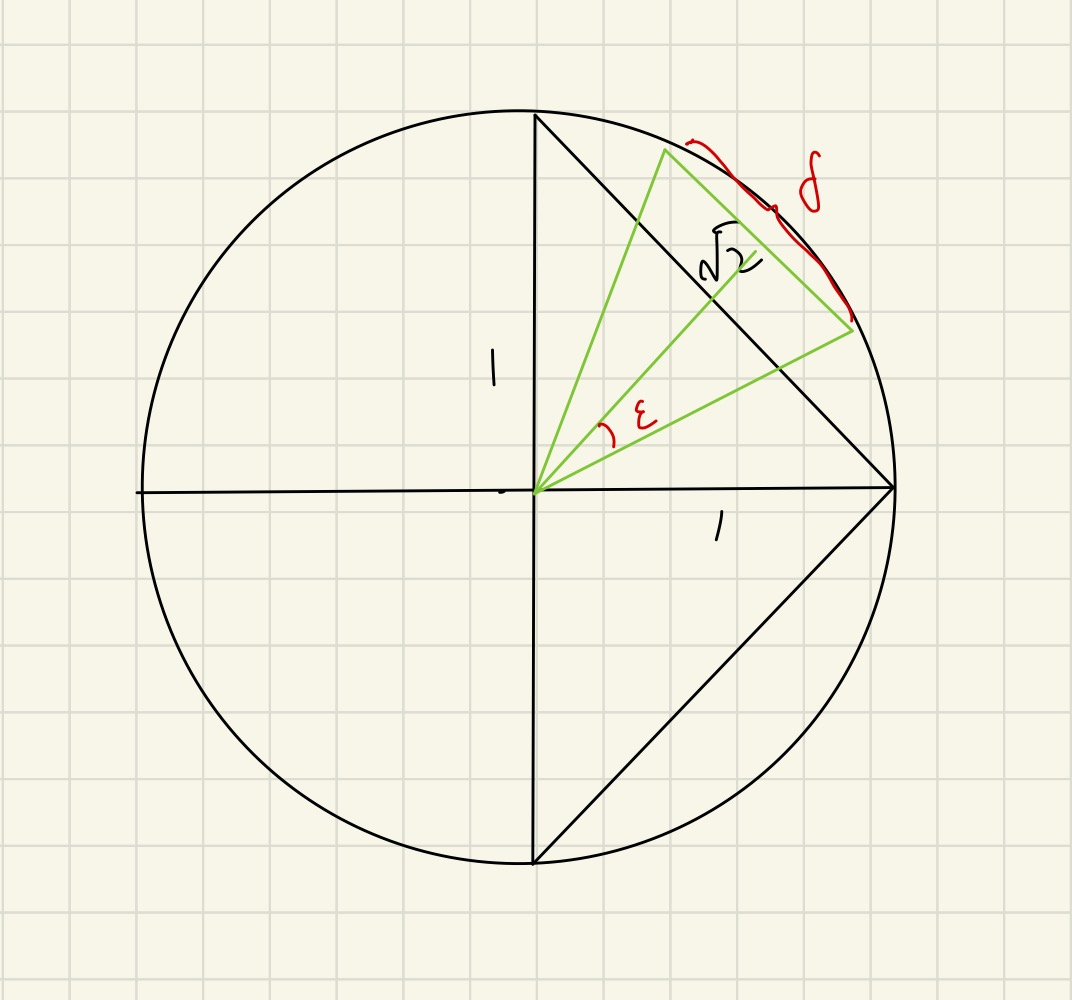
\includegraphics[width=10cm, height=8cm]{images/sp2.jpg}
\end{center}

如何来说明它是一个商映射呢?我们只需要考虑上半球面,即当$\delta < \sqrt{2}$时,$\mathcal{l}$把每一个$P$在$S^2$每个球形邻域$B_\delta(P)$都变成$\mathcal{l}_P$在$\mathbb{R}\mathbb{P}^2$中的球形邻域$B_\varepsilon(\mathcal{l}_P)$,从上图里面我们可以知道$\delta=2 \sin(\frac{\varepsilon}{2})$,即这是一个开映射,所以$\mathcal{l}$是一个商映射.

\begin{center}
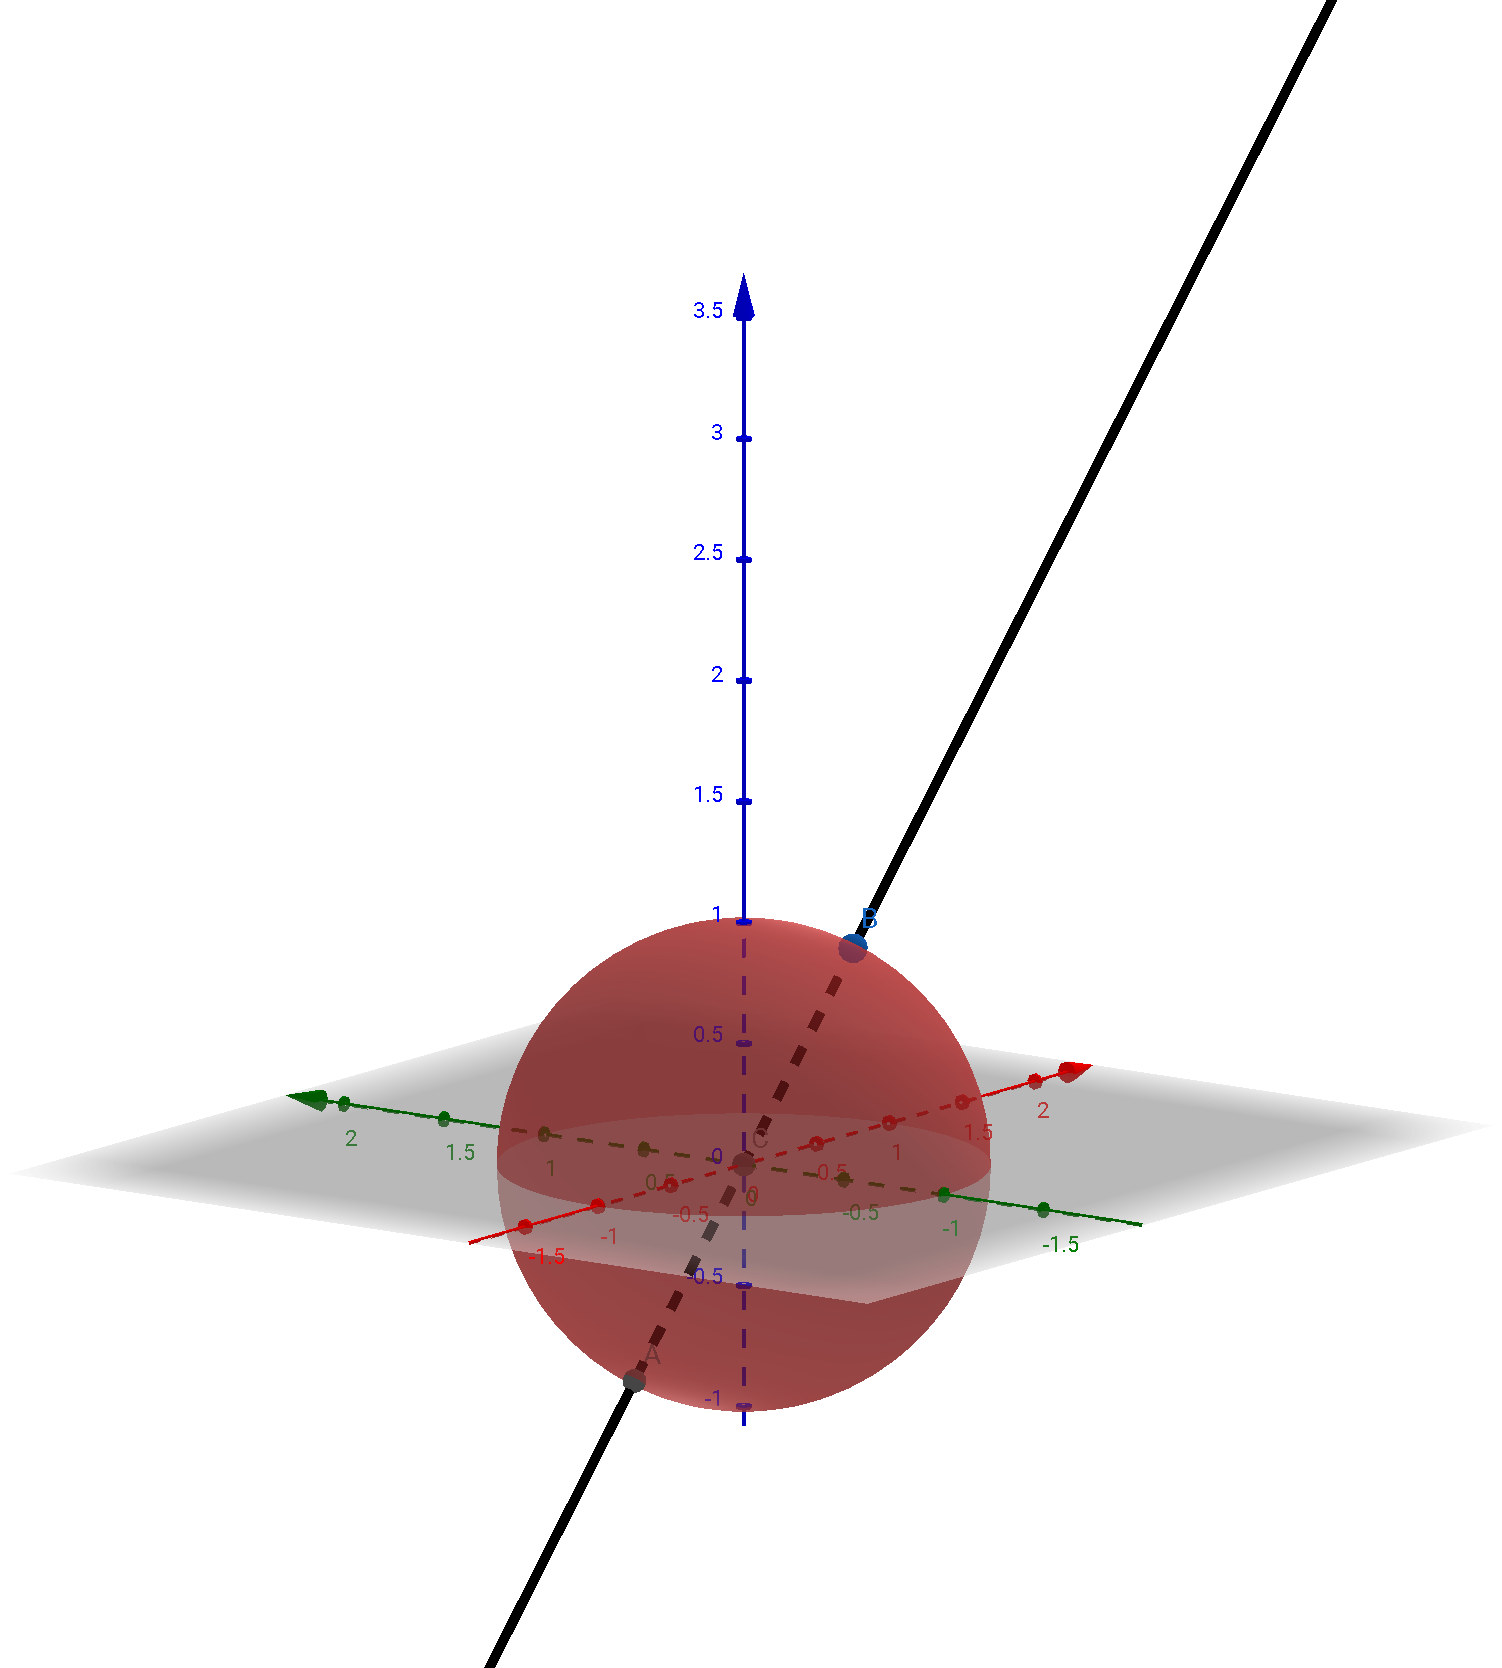
\includegraphics[width=12cm, height=12cm]{images/antipodal_point.png}
\end{center}

对于球面上的每个点$P=(x,y,z)$,$Q=(-x,-y,-z)$称其为\textbf{对跖点}(antipodal point),注意$\mathcal{l}_P=\mathcal{l}_Q$当且仅当$P=Q$或者$P,Q$互为对跖点,因此可以直观的说,射影平面就是“把球面的每一对对跖点粘合成一个点“所得的拓扑空间.

在$\mathbb{E}^3$不能把直线掰弯,关于在$\mathbb{E}^4$中怎么做,留到后面再说...

现在我用前面提到的等价关系来看待"粘合"即商空间,集合上等价关系的定义在这里不想再累述了,我们直接用等价关系来刻画“粘合规则”,那就是: 两个点粘在一起当且仅当它们在同一个等价类里面. 

\begin{definition}
设$\sim$是集合$X$上的一个等价关系,则所有等价类构成的集合称为$X$关于$\sim$的\textbf{商集}(quotient set),记做$X / \sim$. 称映射\[\func{p}{X}{X / \sim},\ x \mapsto \left<x\right>\]为\textbf{粘合映射}(gluing map).若$X$上有拓扑$\tpl$,则称$p$在$X / \sim$上决定的相应的强拓扑为\textbf{商拓扑}(quotient topology),记做$\tpl / \sim$.称拓扑空间$(X / \sim, \tpl /\sim)$为$(X,\tpl)$的\textbf{商空间}(quotient space),记做$(X,\tpl) / \sim$.
\end{definition}

\begin{example}
把一条很长的带子两端粘合起来可以得到平环$S^1 \times [0,1]$或者Mobius带. 利用商空间的语言,现在可以数学上严格地重新定义Mobius带为如下的粘合结果: 考虑$(x,y)$即$[0,1] \times [0,1]$上的子集族\[\mathcal{U}_M = \Set{\{(0,y),(1,(1-y))\}}{y \in [0,1]} \cup \Set{{(x,y)}}{x \in (0,1), y \in [0,1]} \]
\begin{center}
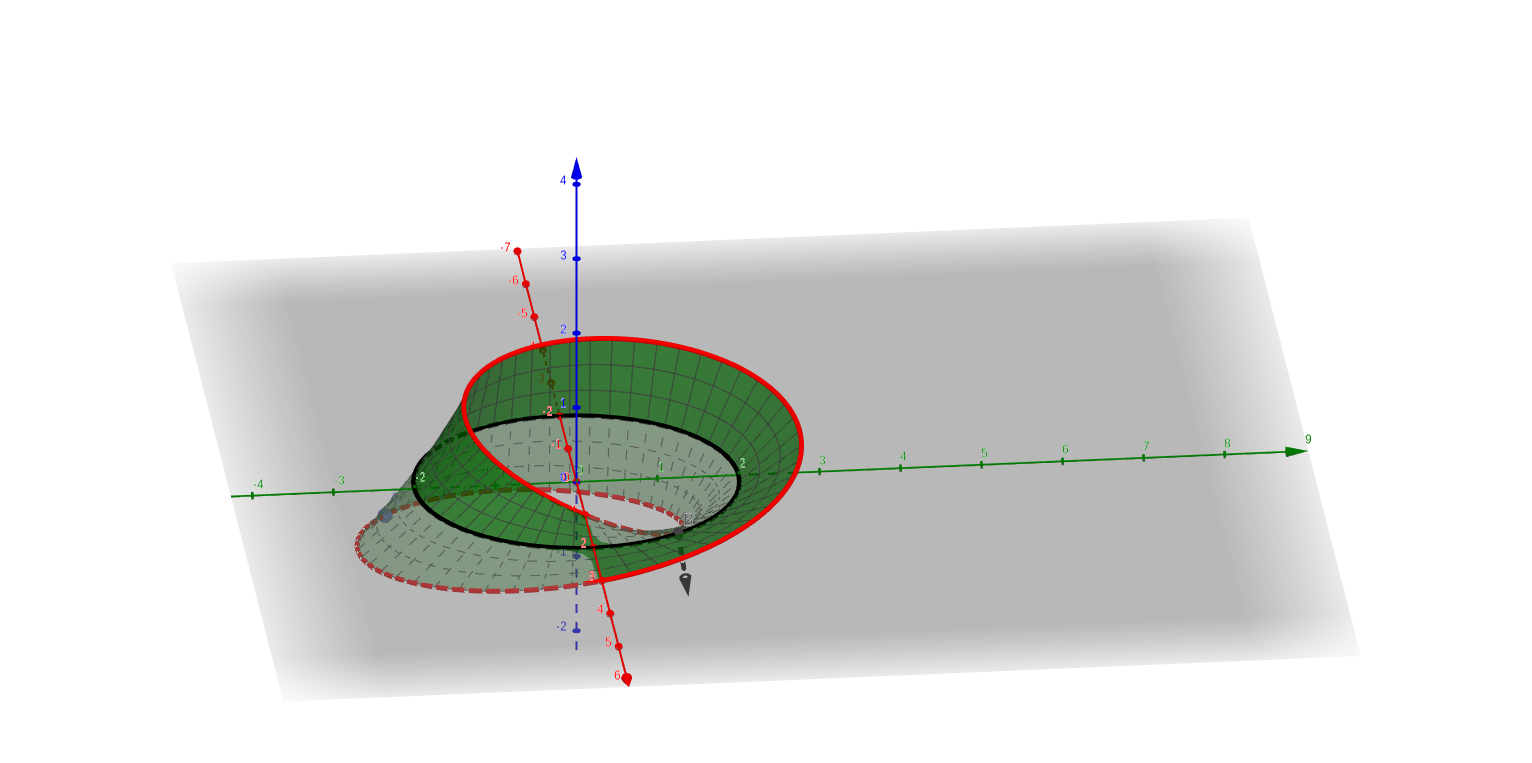
\includegraphics[width=20cm, height=15cm]{images/Mobius.png}
\end{center}
在Mobius带上,我们考虑把带子两边上的点拧半圈,然后粘合到一起,从上面的图可以尝试形象的理解一下. 按照$\mathcal{U}_M$里面划分的等价类,商空间$([0,1] \times [0,1]) / \sim_M$就称为Mobius带.另一方我们考虑下面这种划分方式\[\mathcal{U}_A = \Set{\{(0,y),(1,y)\}}{y \in [0,1]} \cup \Set{{(x,y)}}{x \in (0,1), y \in [0,1]}\],这种划分方式就是把带子两边直觉对着粘起来,参考下面图中紫色的部分,而商空间$([0,1] \times [0,1]) / \sim_A$就是平环.

\begin{center}
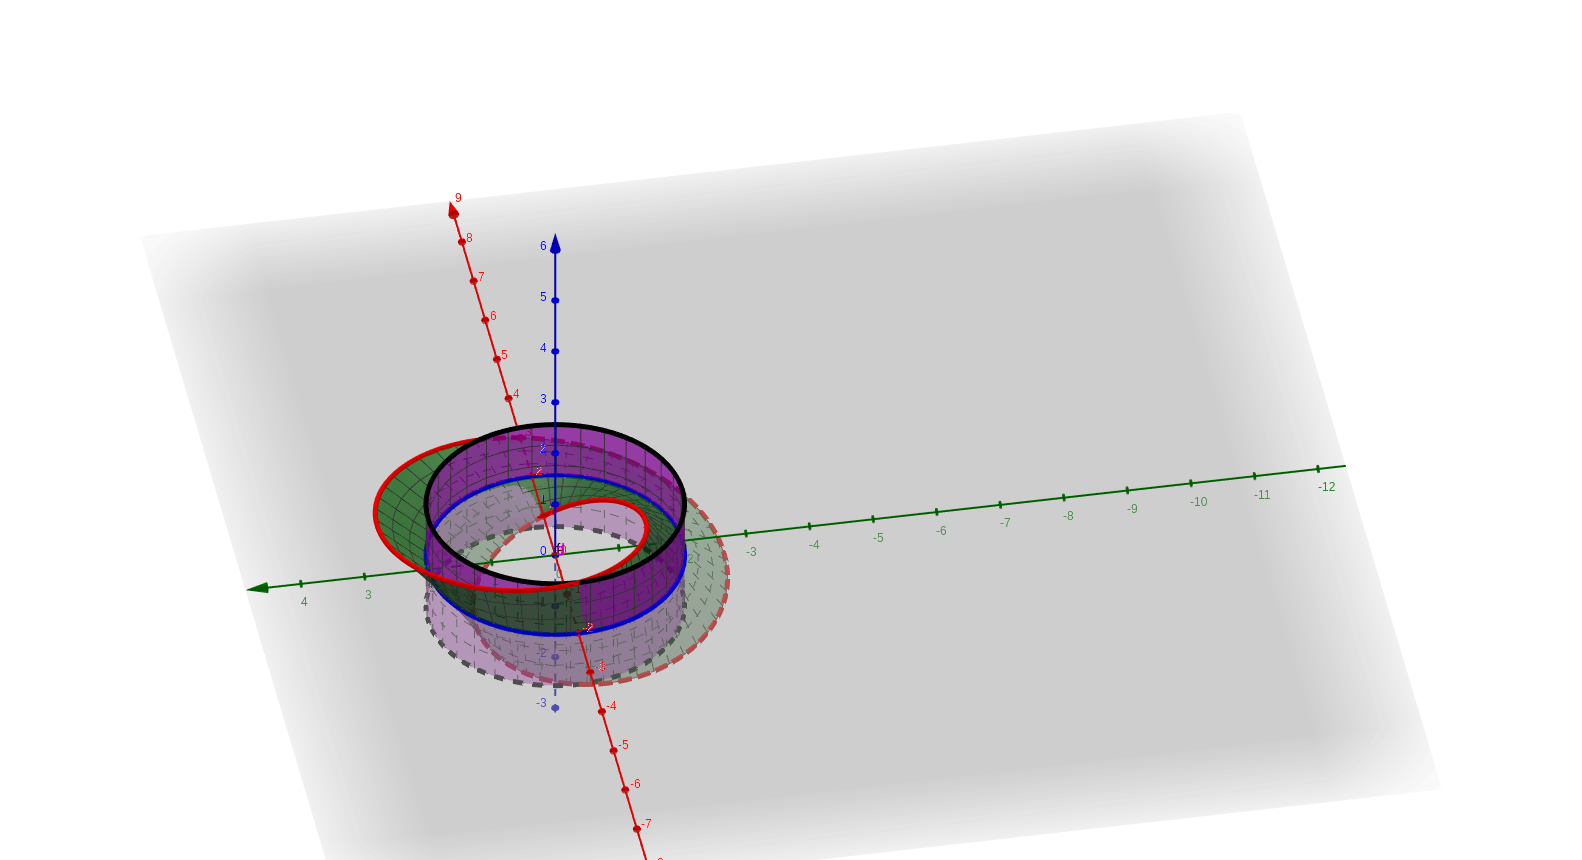
\includegraphics[width=20cm, height=12cm]{images/gluing.png}
\end{center}
\end{example}


\begin{proposition}
商空间里面的子集开当且仅当其关于粘合映射的原像开,言下之意粘合映射是商映射.
\end{proposition}

上面这个命题很显然了,强拓扑加满射(等价关系的基本定义).

\begin{theorem}
设$\func{f}{X}{Y}$是商映射,$\sim_f$是$X$上的等价关系,满足$f(x)=f(x')$当且仅当$x \sim_f x'$. 则商空间$X / \sim_f$与$Y$同胚.
\end{theorem}

\begin{proof}
它来了,同态第一定理?同胚第一定理?哈哈),$f$和$p$都是商映射,且$f(x)=f(x')$当且仅当$p(x)=p(x')$,由定义2.62,$X / \sim_f$和$Y$同胚.
\end{proof}

商空间和商映射本质上考虑的是一样的问题,只不过出发点不同,考虑不同空间之间的映射和相互关系时商映射比较好用,而单纯为了理解空间本身的时候,商空间就比较好用一些. 上述定理给出了两者之间的联系,当我们为一个空间给出了一种“粘合”式的构造方法时,并且想严格说明得到的空间和这个空间原本具有的另一个定义一致(即同胚)时,应用该定理也是一种标准的做法.

还需要一些例子来好好理解一下
\begin{example}
考虑两个不相交的圆的并集\[A=\Set{(x,y) \in \mathbb{E}^2}{(x+2)^2+y^2=1 \text{ 或者 }(x-2)^2+y^2=1\]}在这两个圆上各取一点$p=(-1,0)$,$q=(1,0)$,然后把这两个点粘到一起,得到的空间$S^1 \vee S^1$称为两个圆的\textbf{一点并}(one-point union). 用商空间的语言来讲,$S^1 V S^1=A / \sim$,这里若两点等价$a \sim b$当且仅当$a=b$或者${a,b} = {p,q}.$ 在代数里面要理解关于商的东西,并不直观,例如商环等等,只有通过同构来来间接的描述,同样在这里我觉得也是这样的思想,所以可以另取一个空间\[B=\Set{(x,y) \in \mathbb{E}^2}{(x+1)^2+y^2=1 \text{ 或者 }(x-1)^2+y^2=1}\]两圆相切于一点的并集,然后考虑如下映射
$$
	\func{f}{A}{B},\ (x,y) \mapsto \left\{
    \begin{array}{cc}
           (x+1,y) ,& x<0 \\
           (x-1,y) ,& x>0
    \end{array}
	\right.
$$

容易验证该映射是一个连续满射,考虑$A$中任意点$P$球形邻域,对应$B$中点$P$球形邻域,有点麻烦,但是可以对应上,这样说明它是一个商映射,从上述定理可知$A / \sim_f = B$. $sim_f$和$f$确立的等价关系是相同的,所以$A / \sim = B$.

\begin{center}
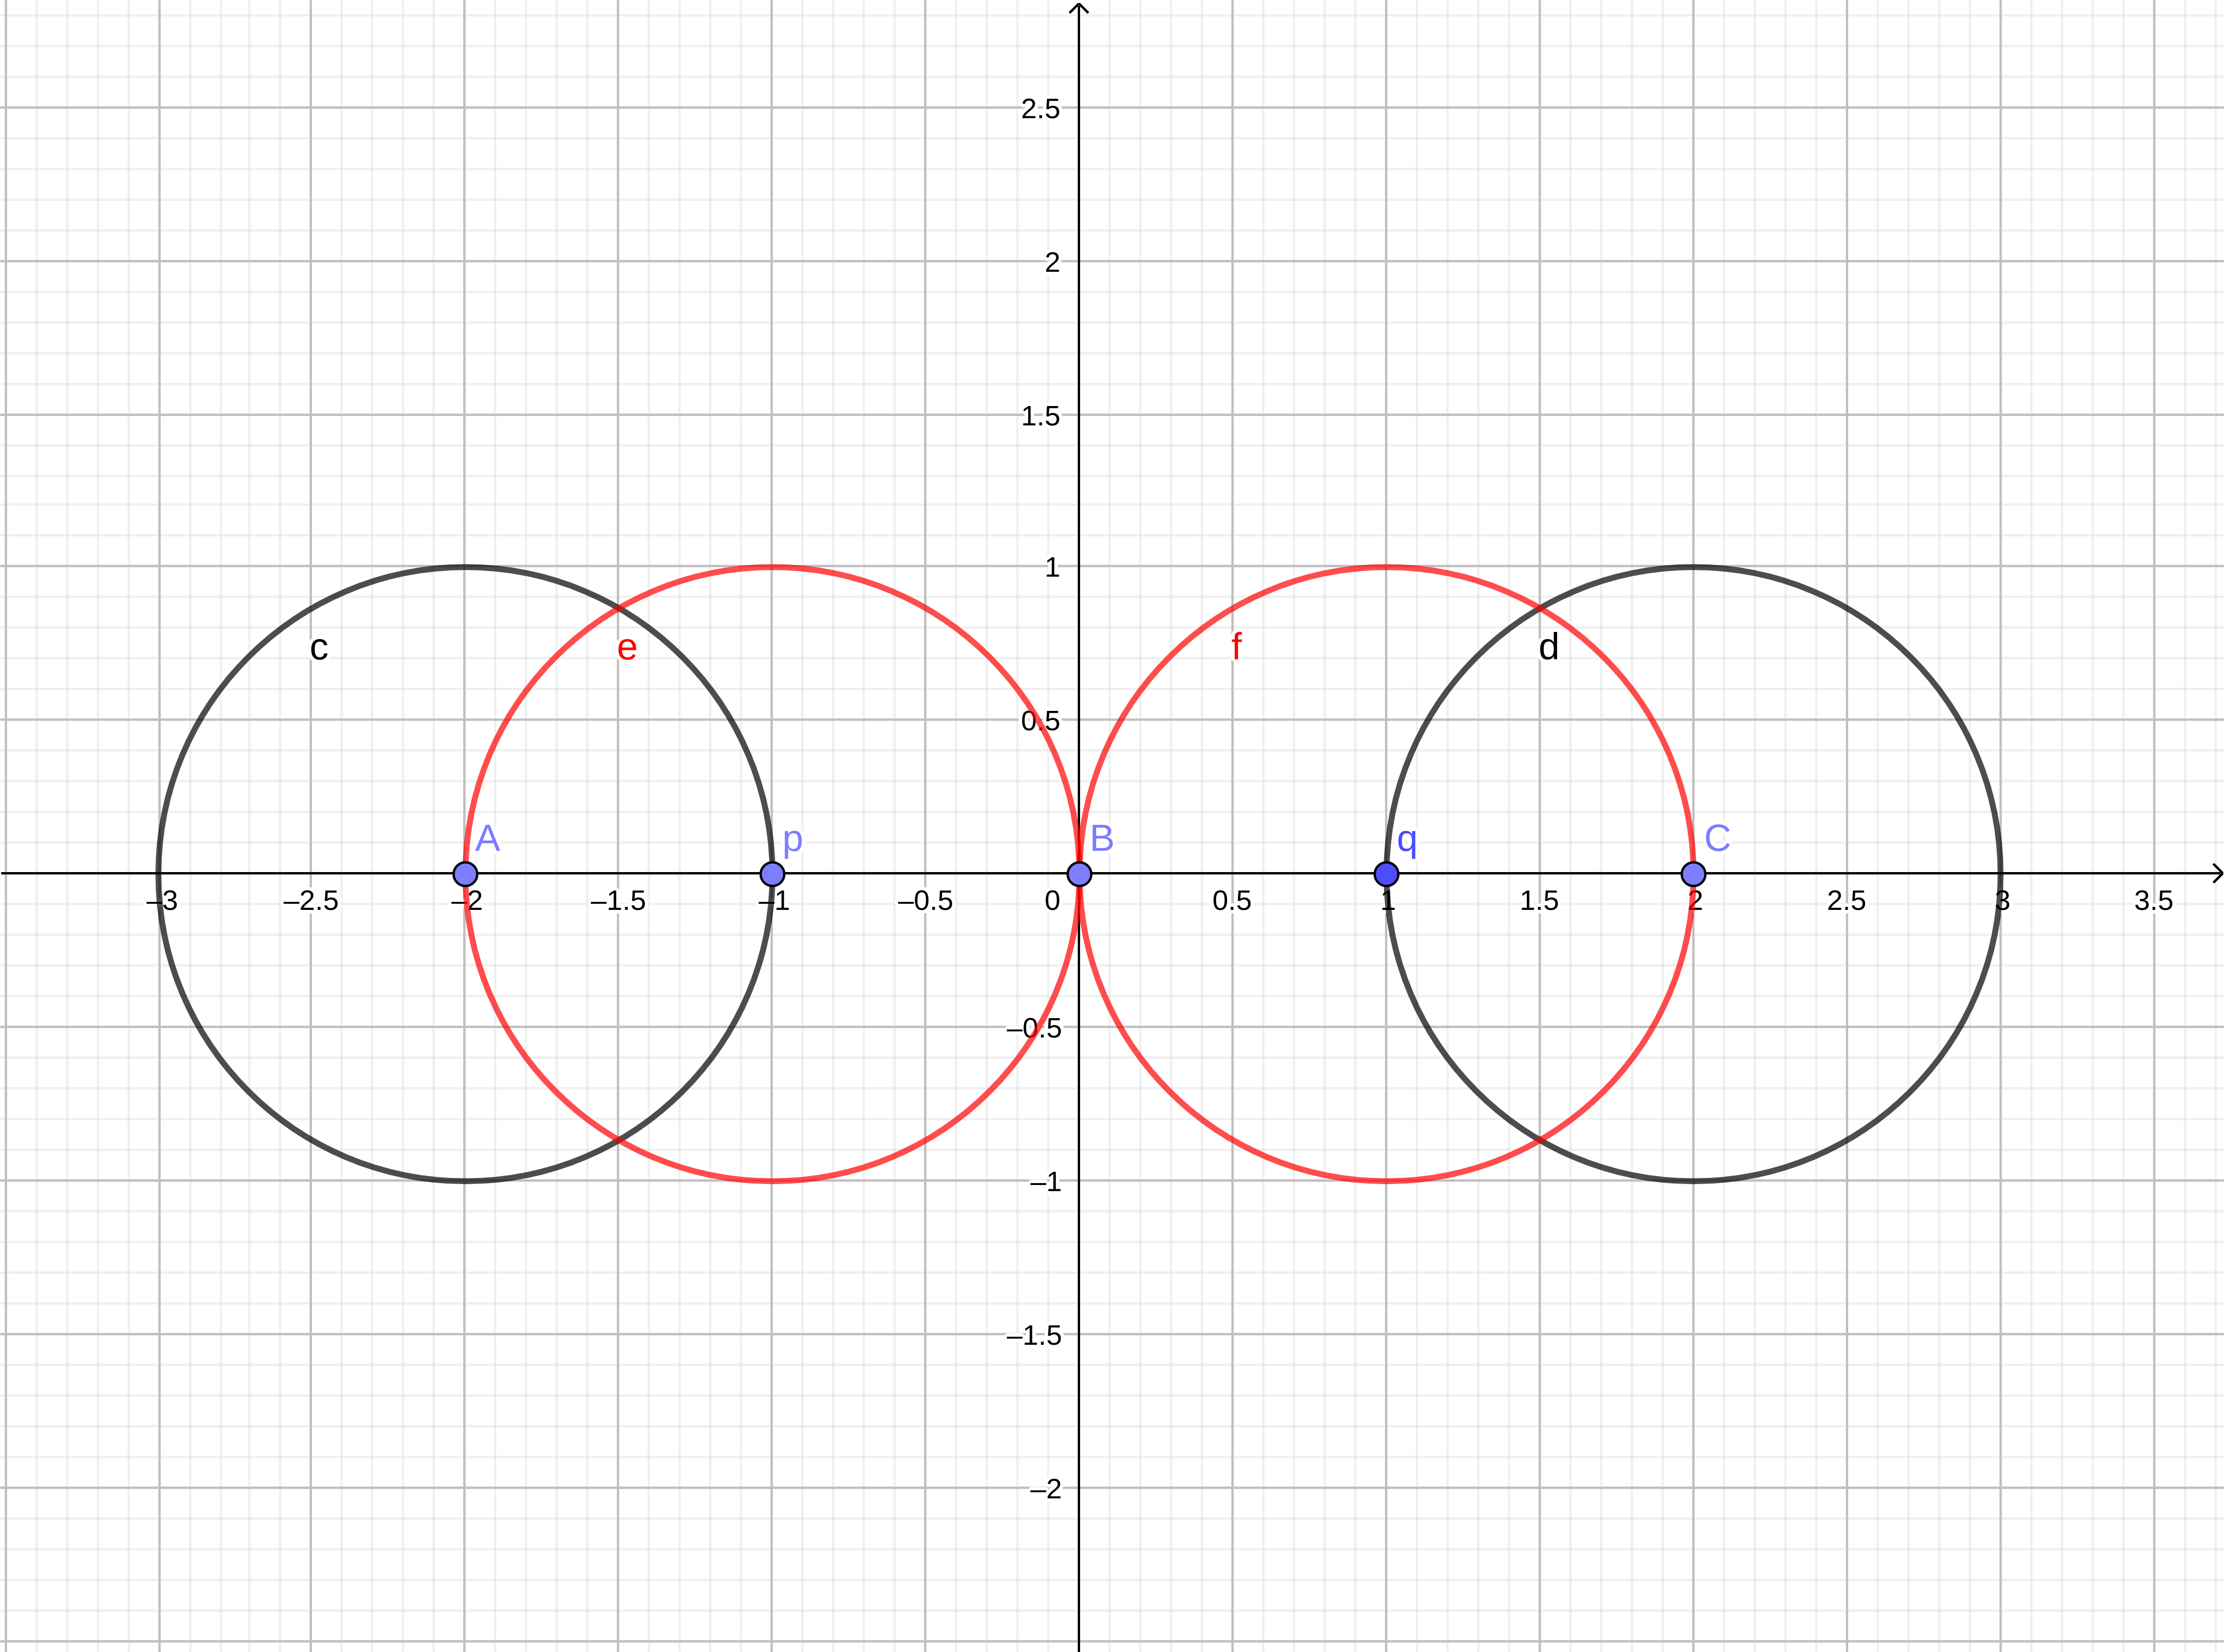
\includegraphics[width=15cm, height=10cm]{images/one-point-union.png}
\end{center}
\end{example}

我们再来用商空间的重新定义一下射影平面,利用商空间的语言,可以把它解释成$\mathbb{R}\mathbb{P}^2=(\mathbb{R}^3 \smallsetminus \{(0,0,0)\}) / \sim$,这里$sim$每一个等价类都是过原点的直线,但是每个等价类都不能相交,所以拿掉了原点,也就是说点$(x,y,z)$所在的等价类是$\Set{(tx,ty,tz)}{ t \neq 0}$.然后再把这个概念推广到高维的情况下.

\begin{definition}
称一个向量空间中的一维子空间维一条\textbf{中心直线}(line through origin). 在$\mathbb{E}^{n+1} \smallsetminus \{0\}$中任取$x=(x_0,\ldots,x_n)$,记其所在的中心直线为$\mathcal{l}_x=\Set{(tx_0,\ldots,tx_n)}{t \in \mathcal{R}}$. 则集合族\[\mathcal{U} = \Set{\mathcal{l}_x \smallsetminus \{0\} }{x \in \mathbb{E}^{n+1} \smallsetminus \{0\}}\]定义了$\mathbb{E}^{n+1} \smallsetminus \{0\}$上的一个等价关系$\sim_{\mathcal{U}}$.商空间\[\mathbb{R}\mathbb{P}^n=(\mathbb{E}^{n+1} \smallsetminus \{0\}) / \sim_{\mathcal{U}}\]称为$n$维实射影空间.特别地,$\mathbb{R}\mathbb{P}^2$就是射影平面.
\end{definition}

想想我们之前定义的射影平面,里面的度量是两条直线的夹角,然后我们建立了一个$S^2$和$\mathbb{R}\mathbb{P}^2$的商映射,用邻域的形式说明了它。在这里我们用“粘合”的观点来看一下它

\begin{example}
射影平面同胚于球面粘合对跖点。
\begin{proof}
考虑映射\[\func{p}{S^2}{\mathbb{R}\mathbb{P}^2},\ x \mapsto \left< x \right>.\],其中$\mathbb{R}\mathbb{P}^2$现在是$\mathbb{E}^3$下的商空间。我们任取$S^2$中的开集$U$,这里记$\mathbb{E}^3$到商空间$\mathbb{R}\mathbb{P}^2$的粘合映射为$\mathcal{l}$,$p(U)$是若干等价类的并,$l^{-1}(p(U))$对应锥形是$\mathbb{E}^3$中的开集,所以$p(U)$开集,即$p$是开映射,从而是商映射.

$\mathbb{R}\mathbb{P}^2$中每个点$x$的原像集$p^{-1}(x)$恰好由球面上的一对对跖点构成.因此球面粘合对跖点所得商空间是同胚于$\mathbb{R}\mathbb{P}^2$.
\end{proof}
\end{example}

\begin{definition}
若拓扑空间$X$上的某个子集$A$,它是某个开集的交集,则称$A$是饱和的(saturated).
\end{definition}

\newpage
\subsection{Misc}

\begin{proposition}
给定集合$X$,子集族$S \subseteq P(x)$, 包含$S$的最小拓扑为$\tpl_S = \Set{U \subseteq X}{\bigcup\limits_{V \in \mathcal{F}} V, \mathcal{F} \subseteq S'}$,其中$S' = \Set{S_1 \cap \cdots \cap S_k}{S_1,\cdots,S_k \in S, k \in \mathbb{N}} \cup \{X\}$.
\end{proposition}

用文字来说就是包$S$的最小拓扑是任意并上$S$里面元素有限的交所构成的. 证明经典两边包含.

\begin{definition}
若拓扑空间上$(X,\tpl)$中的拓扑结构$\tpl = \tpl_S$,也就是说$\tpl$是由$S$导出的,则称$S'$为拓扑空间$(X,\tpl)$的一个\rm subbasis(准基).
\end{definition}

如果我们能只做$S$里面元素的任意交集就能构成一个拓扑那就太好了,哈哈,这个时候$S$其实就是一个basis(拓扑基).

basis 有一个比较好的性质,在证明连续的时候,只需要check basis里面的元素的原像是否开就行,不用check所有的开集.

\begin{proposition}
给定两个拓扑空间$(X,\tpl_S)$,$Y$和它们之间的映射$\func{f}{Y}{X}$,$f$连续当且仅当$\forall s \in S$,$f^{-1}(s)$是$Y$上的开集.
\end{proposition}

英文definition表示我自己翻译有点难看 ((

\begin{definition}
\rm $\mathcal{B}$ is a local base for $(X,\tpl)$ at $x$ iff all $B \in \mathcal{B}$ are open ($\mathcal{B} \in \tpl$)and also contain $x$, and moreover for all $U \in \tpl$ with $x \in U$ there exists some $B \in \mathcal{B}$ such that $B \subseteq U$.
\end{definition}


\begin{proposition}
给定$X$上的子集族$B$,$B$是$X$的一个basis 当且仅当$\forall x \in X$,$B_x$是$X$上$x$的一个local basis.
\end{proposition}

Local homeomorphisms are used in the study of sheaves.

\begin{definition}
\rm 给定两个拓扑空间$X$,$Y$,和它们一个映射$\func{f}{X}{Y}$,若对于$\forall x \in X$,都存在着一个开集$U$包含$x$, 且$f(U)$在$Y$上也是开集,所以把$f$现在在这些$U$上,$f|_U$就是一个同胚,称这样的$f$是一个局部同胚(local homeomorphism)
\end{definition}

\textbf{standard topology} on $\mathbb{R}^n$.
\begin{definition}
$\mathbb{R}^n = \{(x_1,\cdots,x_n)\},x_i \in \mathbb{R}$.
\end{definition}

\begin{definition}
$|x| = \sqrt{\sum x_i^2}$ $d(x,y)=|x-y|.$
\end{definition}

\begin{definition}
\rm 假定$x \in \mathbb{R}^n$,$B_r(x)$表示在点$x$处半径为$r \in \mathbb{R}$的开球(open ball),定义如下\[B_r(x)=\Set{y}{|y-x| < r}.\]
\end{definition}

\begin{definition}
若某个$\mathbb{R}^n$中的子集$A$开当且仅对任意的$x \in A$,存在$\varepsilon > 0$,使得$B_\varepsilon(x) \subseteq A$.
\end{definition}


\begin{definition}
$\mathbb{R}^n$上序列用$(x_i)i\in\mathbb{N}$表示一连串$\mathbb{R}^n$上的元素indexed by natural numbers. 给定一个序列$(x_i)_{i\in\mathbb{N}}$,它的子序列表示为$(x_i)_{i \in I}$,其中$I \subseteq \mathbb{N}$也是一个无限集,经常定义$I = \{i_1,i_2,\cdots\}$,其中$i_1 < i_2 < \cdots$,所以$(x_i)$的子序列可以用$(x_{i_j})_{j \in \mathbb{N}}$.
\end{definition}

点列极限...

\begin{definition}
给定$\mathbb{R}$上的序列$(x_n)$,$(x_i)$收敛于$x \in \mathbb{R}^n$表示为对任意$\varepsilon > 0$,存在$N \in \mathbb{N}$,使得当$i > N$时$|x_i - x| < \varepsilon$.
\end{definition}

\begin{proposition}
序列$(x_i)$ 收敛于$x$,则其所有的子序列都收敛于$x$.
\end{proposition}

\begin{definition}[R-saturated]
$X$是一个集合,$R$是$X$上的一个等价关系,若子集$X$上的子集$A$满足$\forall x \in X, a \in A$,如果$xRa \Rightarrow x \in A$,则称$A$是一个饱和子集(R-saturated)
\end{definition}

saturated有点像环里面的ideal,它可以吸收与它里面元素等价的其他元素.

\newpage
\section{General Topology}
\subsection{Basis and Countable Axiom}

\begin{definition}
拓扑空间$X$中点$x$的一个\textbf{邻域基}(neighborhood base)指由$x$的邻域构造成的子集族$\mathcal{N}_x$,使得$x$的任何邻域均包含$\mathcal{N}$中的某个邻域.
\end{definition}

回想一下前面定义的基准开邻域,包含一个基准开邻域的子集是邻域,所以基准开邻域结构天然构造了一个领域基.

\begin{definition}
如果点$x$的一个邻域基$\mathcal{N}_x$只含有可数个成员,则称之为$x$的可数邻域基(countable neighborhood base).如果拓扑空间$X$中的每个点都拥有一个可数邻域基,则称$X$为第一可数空间,该条件称为第一可数公理.
\end{definition}

\begin{example}
度量拓扑空间都是第一可数空间,因为对每个点$x$来说,$\mathcal{N}(x)=\Set{B_{\frac{1}{n+1}}(x)}{n\in \mathbb{N}}$就是它的一个可数邻域基.
\end{example}

怎么理解上面例子呢?任取$\varepsilon \in \mathbb{R}$且大于0,然后取$\varepsilon$最高位,发现它都可以包含一个有理数,而有理数是可数的。

上面这个例子也说明可数公理与这个空间是否只含可数个点并没有什么关系. 反过来只含有可数多个点的空间也可以不满足第一可数公理,比如Appert构造的下述反例

\begin{example}
让$X$为正整数集,让$N(n,E)$表示$E \subseteq X$中小于等于$n$的元素个数.在它基础上定义Apperts拓扑,若$E$属于该拓扑,则$1 \notin E$或者$1 \in E$且$\displaystyle \lim_{n \mathop \to \infty} \dfrac {{N}{(n, H}) } n = 1$,这个拓扑空间不是满足第一可数公理.
\end{example}

\begin{proof}
怎么理解这个拓扑空间呢?它是满足基准开邻域的,不要去想它的内部东西,直接套公理即可,是容易证明的。

如何证明它不满足第一可数公理呢?我们去一个特殊的子集$\Set{2^n}{n>=1}$,这是一个无限集,其中每个点都是独立离散的,所以每个点至少有一个不同的基准邻域,所以弄在一起邻域基是可数的.
\end{proof}

当然了,很多实际应用中遇到的空间都满足第一可数公理(比如度量空间). 当一个空间满足第一可数公理时,我们可以对每个点的邻域使用数学归纳法,从而得到一些漂亮的结果.

\begin{proposition}
若$x$有一个可数邻域基,则$x$有一个可数邻域基${V1,V2,\cdots}$,使得当$m > n$,总有$V_m \subseteq V_n$
\end{proposition}

这个命题反过来似乎在告诉我们,可数邻域基可以由一个最小的邻域,不断的填充,变成新的邻域,再把这些邻域合起来就是新的邻域基,那么如何取最小的邻域呢? 所有这样的邻域交一下不就是吗?下面严格证明。

\begin{proof}
若$x$有一个可数邻域集,则$x$有一个可数邻域基$\{U_1,U_2,\cdots\}$,令$V_n=U_1 \cap \cdots \cap U_n$,这样当$m>n$是,一定有$V_m \subseteq V_n$,然后再证明它是一组邻域基,由已知的邻域基有任取$x$邻域$U$,存在某个正整数$n$,使得$U_n \subseteq U$, 因为$V_n \subseteq U_n$,所以$V_n \subseteq U$.
\end{proof}

这个命题让邻域基有一种序的关系,这有作用呢?把邻域基想象成圆环套圆环的图形,每个圆环在无限的“逼近”圆心,也就是相当于圆心的有任意长度的圆心,一个圆环就是一个邻域,如果我在每个圆环里面取一个点,构成一个点列,这列点列将无限的靠近圆心.我们遵循这个思路来想想下面的东西.

下面一些包包老师书的掺杂邻域的东西,感觉很模糊,但是还是记录一下,比较不同的视角也许能发现一些新的东西.
\begin{definition}
设${x_n}$是一个点列,若点$x$满足任取$x$的邻域$U$,存在自然数$N$,使得当$n > N$时每个$x_n$都在$U$中,则称$x$为点列${x_n}$的一个\textbf{极限}(limit).
\end{definition}

数学分析中的数列极限的推广,把里面的$\varepsilon$变成了一般性的邻域$U$可刻画.在数学分析中聚点的定义是若点$a$的任意去心邻域内都有数集$A$中的点,就称点$a$就是数集$A$的聚点(accumulating point).用形式语言来描述就是\[\forall \delta > 0,\exists x \in A \colon 0 < |x-a| < \delta.\].在拓扑学里面来描述就是在拓扑空间$X$下,若$A$是$X$的某个子集,取$x \in X$,若$x$的每个邻域都含有$A \smallsetminus \{x\}$的点,则称$x$是$A$的聚点.这里有一个聚点另外一种形式的刻画

\begin{proposition}
设$x \in X$有可数邻域基,$A \subseteq X$,则$x$是$A$的聚点当且仅当存在由$A \smallsetminus {x}$中的点构成的点列${x_n}$以$x$为极限.
\end{proposition}

\begin{proof}
从数分里面的定义,看起来确实像可以取定一个数列,它的极限点. 来严格证明一下,若$x$是$A$的聚点,怎么来构造一个点列让它的极限是$x$呢?从上一个命题里面我们可以找一个$x$的可数邻域为$\{V_1,V_2,\cdots\}$使得$m > n$时$V_m \subseteq V_n$,然后在分别在$V_n \cap A$取一点$x_n \neq x$(聚点的定义是每个邻域都有$A$中的点),则以点列${x_n}$以$x$为极限.

反过来存在$A \smallsetminus \{x\}$中的点列${x_n}$以$x$为极限,则当$n >N$时,$x$的任何邻域都要包含某个$x_n \in A \smallsetminus \{x\}$,因此$x$是$A$的聚点.
\end{proof}

聚点和极限本质上刻画的是同一个东西,都是有无穷多个点聚在某处,数分里面的聚点是针对某个数列,而现在直接给你一个子集,要说明子集的聚点?这个就不唯一了,你可以从这个子集里面取很多个点列出来。

%对应上面命题的理解,其实就是在$A$里面画圈,在圈里面描点,反过来就是靠点列把圆圈再还原出来。

%我们用前面的思路来重新理解一下,把$x$想象成圆心,按照聚点基本定义,$x$的任何去心邻域都有$A$的里面点才行,相当于$A$是包含$x$集合,且$A$一定要包含某个$x$的基邻域,相当于要把$A$和这些圆环串在一条“直线”上,这条直线用$\{x_n\}$来描述,好吧这些都是一些我自己理解,也许不对 (.

还有一个用极限来刻画连续的命题

\begin{proposition}
设$x \in X$有可数邻域基,则映射$\func{f}{X}{Y}$在$x$点处连续的充分必要条件是: 任取以$x$为极限的点列$\{x_n\}$,点列$\{f(x_n)\}$都以$f(x)$为极限.
\end{proposition}

\begin{proof}
很优雅的结论,若$f$连续,然后取以$x$为极限的点列$x_n$,在任取$f(x)$的邻域$U$,根据极限的定义,当$n > N$时,有$x_n \in f^{-1}(U)$,从而$f(x_n) \in U$,则以$\{f(x_n)\}$为点列的极限是$f(x)$.

反过来,取$x$的可数邻域基$\{V_1,V_2,\cdots\}$使得$m > n$时总有$V_m \subseteq V_n$,任取$f^{-1}(x)$的邻域$U$,假设$f(U)$不是$x$的邻域,则我们可以在前面可数邻域基里面取这样一组点$x_n \in V_n \smallsetminus f^{-1}(U)$,为什么可以取到这样一组点呢?因为当$f^{-1}(U)$不是$x$邻域的时候$f^{-1}{U}$不包含任何可数邻域基里面的成员. 取到这样的一组点同样是以$x$为极限的点列,但是它$f(x_n)$并不含于$U$,所以$\{f(x_n)\}$以$f(x)$为极限不成立,与条件矛盾,所以$f^{-1}(U)$是$x$的邻域.
\end{proof}

如何来理解和记忆这个命题呢?这个证明也很绕,有没有一种很直观的理解来描述这一奇特的连续条件呢?

\begin{center}
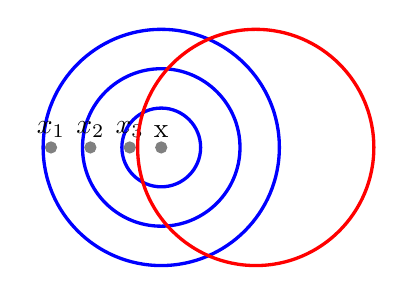
\begin{tikzpicture}
\foreach \i in {1,...,3}
{
	\draw[blue, very thick] (-1,0) circle (0.5*\i);
	\pgfmathsetmacro{\mynum}{int(4-\i)};
	\draw (-0.5*\i-0.9,0) node[above]{$x_{\mynum}$};
	\filldraw [gray] (-0.5*\i-0.9,0) circle (2pt);
}

\draw[red, very thick] (0.2,0) circle (1.5);
\draw (-1,0) node[above]{x};
\filldraw [gray] (-1,0) circle (2pt);
\end{tikzpicture}
\end{center}

如果$f^{-1}(U)$不是$x$的邻域,则它不包含任何邻域基里面的成员,也就是如上图,接着我们可以找到以$x$为极限的点列$\{x_n\}$它不在$f^{-1}(U)$,随之$f(x_n)$ 也不在$U$里面.

注意上面命题的开头都是$x$有可数邻域基,主要是为了取可数点列. 

邻域基是一种挑出一部分邻域来“代表”所有邻域的机制,类似地,也有一种挑出一部分开集来“代表”所有开集的机制,称为拓扑基.

\begin{definition}
设$\mathscr{B}$是集合$X$上的一个子集族,称子集族\[\overline{\mathscr{B}}=\Set{U \subseteq X}{U \text{ 是 } \mathscr{B} \text{ 中若干成员的并集 }}\]为$\mathscr{B}$\textsf{生成}(generate)的子集族,若$\bar{\mathscr{B}}$恰好是拓扑空间$(X,\tpl)$上的拓扑结构$\tpl$,则称$\mathscr{B}$为其\textbf{拓扑基}(topological base).
\end{definition}

设$\mathcal{N}$是$X$上一个生成拓扑结构$\tpl$的基准开领域结构,则$\mathscr{B}=\bigcup\limits_{x \in X}\mathcal{N}(x)$就是一个拓扑基.

拓扑基另一个定义是它是一个开集族,这个定义更强调了拓扑基一定是相对于某个拓扑结构.生成是什么意思呢?是只取其中一部分元素来生成还是要取到所有的元素?若要和前面拓扑基的另一个定义对应上,这里要取到所有元素来生成. the collection of all unions of members of $\overline{\mathscr{B}}$.


那么问题来了,如果我们给定$X$上的一个子集族,如何判定这个子集族是不是一个拓扑基?

\begin{proposition}
设$\mathscr{B}$是集合$X$上的一个子集族,则$\overline{\mathscr{B}}$是$X$上拓扑结构的充分必要条件是
\begin{enumerate}
	\item $\bigcup\limits_{B \in \mathscr{B}}B = X$;
	\item $\forall B_1,B_2 \in \mathscr{B},B_1 \cap B_2 \in \overline{\mathscr{B}}$
\end{enumerate}
\end{proposition}

想想$\overline{\mathscr{B}}$本身的性质,其中$\emptyset$肯定在里面,因为empty union,任意的并也是封闭,所以只需要保证$\overline{\mathscr{B}}$在交运算下封闭,这就是上述的命题主要刻画的剩余条件.这个命题很有作用,能帮我们快速的判定一些拓扑基.

\begin{example}
给定$\mathbb{R}^2$上一块不带边的长方形$a < x < b, c < y < d$,让$\mathscr{B} = \Set{<x,y>}{<x,y> \in \mathbb{R}^2, a<x<b,c <y <d}$表示所有$(x,y)$和$(a,c)$确定"open rectangles",则$\mathscr{B}$是这块长方形的一个欧式拓扑,用上面命题检验一下.
\end{example}

\begin{definition}
如果拓扑基$\mathscr{B}$只含可数多个成员,则称之为\textbf{可数拓扑基}(countable topological base).若某拓扑空间上存在可数拓扑基,则称其拓扑空间为\textbf{第二可数空间}(second-countable space)或者满足\textbf{第二可数公理}(second axiom of countability)
\end{definition}

相比于第一可数公理,第二可数公理是相对于整个拓扑空间来说的。

\begin{example}
$n$维欧式空间$\mathbb{R}^n$是第二可数空间: 令\[\mathscr{B}=\Set{B_{\frac{1}{k+1}}(x_1,\cdots,x_n)}{k \in \mathbb{N},\text{ 每个 } x_i \in \mathbb{Q}}\]则它是就是一个可数拓扑基(注意这里是$\mathbb{Q}$不是$\mathbb{R}$)
\end{example}

\begin{proof}
每一个的$p \in \mathbb{R}^n$的领域,都可以找到一个$x \in \mathbb{Q}^n$包含这个点$p$,$\mathbb{Q}^n$球形领域是可数的。
\end{proof}

\begin{example}
$\mathbb{R}$上的离散拓扑不满足第二可数公理. 对于它的任何拓扑基$\mathscr{B}$来说,每个单点集$\{x\}$因为是开集且它们是含于是$\mathscr{B}$,而这样的单点集有不可数多个(因为$\mathbb{R}$不可数),则$\mathbb{R}$也有不可数多个成员.
\end{example}

第二可数空间一定是可数第一空间,但是反过来不一定成立,离散拓扑可以由度量拓扑诱导出来,而度量空间一定是第一可数空间,$R$上离散拓扑就刚好是这个反例.

\begin{proposition}
第二可数空间可分.
\end{proposition}

\begin{proof}
回顾一下可分的概念,就是指$X$上存在可数稠密子集,稠密是指这个子集的闭包等于全空间.那么我们来先构造一个这样的子集,设$\mathscr{B}={U_1,U_2,\cdots}$是一个可数拓扑基,然后分别从其成员$U_n$取一个$x_n$,构成一个子集$A={x_1,x_2,\cdots}$,$X$上的所有开集都要包含$A$中的某个点,这就说明$X$中的每个点都是$A$闭包中的点,即子集$A$是稠密.
\end{proof}

\begin{proposition}
可分度量空间是第二可数空间
\end{proposition}

\begin{proof}
设$A$是$X$上的一个稠密子集,我们构造一个可数的拓扑基\[\mathscr{B}=\Set{B_{\frac{1}{n+1}}(a)}{a \in A,n \in \mathbb{N}}\],然后我们来证明$X$上的任意开集$U$都是它们并起来的.

任取$x \in U$,是存在合适的$n$使得$B_{\frac{1}{n}} \subseteq U$,因为$A$是稠密的,所以我们取的到$a \in B_{\frac{1}{n}} \cap A$,也是可以找到合适的$n'$使得$x \in B_{\frac{1}{n'}}(a) \subseteq U$,由于$x$是任意的,把这些$B_{\frac{1}{n'}}(a)$都并起来就是$U$.
\end{proof}

延伸一下拓扑基相关概念,前面我们知道了怎么去判定一个子集族是不是拓扑基,也就是去检验这个子集族能不能构造出某个拓扑结构,这种情况下有可能不同的拓扑基对应不同拓扑结构. 那么现在我如果给定一个先给定$X$上的一个拓扑结构$\tpl$,让你取找$\tpl$的拓扑基,这个时候应该怎么找呢?或者换句话说,我们构造了一个拓扑基,我们怎么判定这个拓扑基生成的拓扑是不是恰好$\tpl$?

\begin{proposition}
给定一个拓扑空间$(X,\tpl)$,如果$X$上\textbf{开子集}族$\mathscr{B}$是$\tpl$的拓扑基当且仅当任取$\tpl$的任意一个开集$U$,再任取$x \in U$,总存在$B \in \mathscr{B}$使得$x \in B \subseteq U$.
\end{proposition}

\begin{proof}
若$\mathscr{B}$是$\tpl$的一个拓扑基,则对于任意$U \in \tpl$,有$U = \bigcup\limits_k B_k$,其中$B_k \in \mathscr{B}$,若取$x \in U$,则能找到某个$x \in B_k$,所以$x \in B_k \subseteq U$.

若任取$\tpl$中开集$U$,$x \in U$,总有$B \in \mathscr{B}$使得$x \in B \subseteq U$,取遍$U$里面的所有元素,则$U = \bigcup\limits_k B_k$,则$\mathscr{B}$是一个拓扑基.
\end{proof}

还有一个用拓扑基来判定开集的一个命题:

\begin{proposition}
定义$\mathscr{B}$为$(X,\tpl)$的一个拓扑基,若$X$上某个子集$U$开当且仅当$\forall x \in U$,总存在一个$B \in \mathscr{B}$,使得$x \in B \subseteq U$.
\end{proposition}

我们再考虑一种非常特殊的情况,我们知道拓扑基是不唯一,若$\mathscr{B}$是$(X,\tpl)$上的拓扑基,往$\mathscr{B}$里面再加几个开集,它还是一个拓扑基,这个很显然。那么现在我有两个拓扑基$\mathscr{B}_1$和$\mathscr{B}_2$,如何判定它们生成是同一个拓扑结构还是不同的拓扑结构?

\begin{proposition}
定义拓扑基$\mathscr{B}_1$和$\mathscr{B}_2$分别是拓扑结构$\tpl_1$和$\tpl_2$的拓扑基,若$\tpl_1 = \tpl_2$当且仅当
\begin{enumerate}
	\item $\forall B_1 \in \mathscr{B}_1$和$\forall x \in B_1$,总是存在$B_2 \in \mathscr{B}_2$,使得$x \in B_2 \subseteq B_1$;
	\item $\forall B_2 \in \mathscr{B}_2$和$\forall x \in B_2$,总是存在$B_1 \in \mathscr{B}_1$,使得$x \in B_1 \subseteq B_2$
\end{enumerate}
\end{proposition}

经典的两边相互包含证相等,这个命题非常有趣,例如$n$维欧式空间上的开等边三角形(open equilateral triangle)拓扑基和开长方形(open  rectangle)拓扑基都可以生成欧式拓扑.就可以用上述的命题来刻画它们分别定义的拓扑结构关系,非常有趣.

\newpage

\subsection{Separation Axiom}

这一章主要刻画的是分离公理,分离公理的原意是指是否可以用拓扑结构分离空间中的两个原本不应该重叠的部分.按照对“不该重叠的两部分”理解不同以及区分方法的不同,有很多种不同判定方法和条件,每一种条件被称为一种\textbf{分离公理}(separation axiom).

前面我们提到过的$\text{T}_0$或者$\text{T}_1$就在这里出现了,数学家意识到这些性质有共同之处,值得放在一起研究之前,每个数学家在需要某种形式的此类性质时,都会根据自己的具体需要去写相关的条件,于是赋予了这些分离公理各种不同的名字. 不过现在人们用T加数字下标来对它们统一命名. 字母T来自于德语的分离公理“	das Trennungsaxiom”. 这些公理相互之间没有谁蕴含谁的关系,不过在假设单点集是闭集的前提下编号越大的公理要求越强. 

回忆一下$T_0$空间,对于任意的两点$x$和$y$,存在一个开集只含有$x$,$y$中的一个点.对于存在开集只含有$x$,$y$中一个点,这种条件下,称$x$和$y$可拓扑区分(topologically distinguishable). $\text{T}_0$公理就可以简化为任意两点都可以拓扑区分,这是一个非常弱的条件,虽然弱就意味着很多空间满足它,但是也有缺点,就是用起来很不方便: 当我们讲一个开集“区分”了$x$和$y$的时候,只看这句话甚至无法推断出$U$到底是包含$x$还是$y$.

\begin{definition}
任取$x \neq y \in X$,存在开集$U$,$V$使得$x \in U$,$y \in V$,$U \cap V = \emptyset$,简单来说就是不同的点存在不相交的开邻域,这个条件称为$\rm T_2$公理. 满足$\rm T_2$公理称为\rm\textbf{Hausdorff}空间.
\end{definition}

\begin{proposition}
\rm Hausdorff空间中的每个单点集$\{x\}$都是闭集。
\end{proposition}

\begin{proof}
我们只需要说明$X \setminus \{x\}$是一个开集,即$X \setminus \{x\}$是其中每个点的邻域,任取一个$x \in X$,然后再任取$y \neq x \in X$,由$\rm T_2$公理,$y$必有必有领域包含于$\{x\}^c$,由于$y$是任意的,所以$X \setminus \{x\}$是一个开集,从而$\{x\}$是一个闭集.
\end{proof}

\begin{example}
度量空间都是\rm Hausdorff空间,因为任取$x \neq y$,只需要令$\varepsilon = \frac{1}{2}d(x,y)$即可,想象两个相切的圆.
\end{example}

\begin{proof}
严格证明一下上述取法得到的确实是两个不相交的邻域,假设有一点$p$在同时在这两个邻域里面,则\[d(x,p) + d(y,p) <= 2\varepsilon\]这与度量空间中的三角不等式矛盾,所以不存在这样的点.
\end{proof}

再来一个$\rm T_3$公理

\begin{definition}
如果对任意的闭集$A$和其外一点$p$,存在不相交的开集$U$和$V$使得$A \subseteq U$,$p \in V$,则该空间也叫\rm \textbf{regular} space.
\end{definition}

\begin{definition}
若\rm Hausdorff空间$X$的每个点都有一个邻域同胚于$\mathbb{E}^n$的开子集,则称$X$为一个(不带边界的)\textbf{流形}(manifold),$n$称为这个流形的\textbf{维数}(\rm dimension).
\end{definition}

%流形似乎还没有到它

与$\rm T_2$公理类似还有一个$\rm T_4$公理,但是$T_4$要用拓扑信息区分的对象不是点了,而是不相交的闭集.

\begin{definition}
任取闭集$A$,$B$使得$A \cap B = \emptyset$,存在开集$U$,$V$使得$A \subseteq U$,$B \subseteq V$并且$U \cap V = \emptyset$.简而言之就是不相交的闭集有分别包含它们的不相交的邻域,称为$\rm T_4$公理. 满足$\rm T_4$的空间称为\textsf{正规空间}(\rm normal space).
\end{definition}

这几个分离公理条件是越来越强,可以用下面一张图来形象的描述


\begin{center}
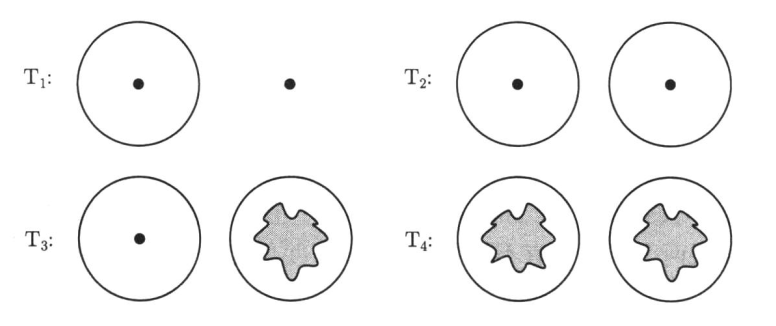
\includegraphics[width=14cm, height=6cm]{images/separation-axiom.png}
\end{center}


%http://math.uchicago.edu/~may/REU2013/REUPapers/Clarke.pdf
\begin{proposition}
度量空间是正规(normal)空间
\end{proposition}

\begin{proof}
设$X$是个度量空间,任取两个不相交的闭集$C_1$,$C_2$,怎么来形象的刻画两个闭集不相交呢?首先定义两个闭集的距离$d(C_1,C_2)=\inf\Set{d(x_1,x_2)}{x_1 \in C_1,x_2 \in C_2}$(可以思考一下这里为什么要取下确界,不能取min呢?),所以$d(C_1,C_2)>0$,我们可以定义两个分别包含它们的开集 
\begin{align} 
U_1 = \bigcup\limits_{x \in C_1}\frac{B_{d(C_1,C_2)}}{3}(x) \\ 
U_2 = \bigcup\limits_{x \in C_2}\frac{B_{d(C_1,C_2)}}{3}(x) 
\end{align}
为了说明$U_1 \cap U_2 = \emptyset$,假设它们相交,任取一点$y \in U_1 \cap U_2 $,则肯定存在$x_1 \in C_1$和$x_2 \in C_2$使得\[y \in \frac{B_{d(C_1,C_2)}}{3}(x_1) \cap \frac{B_{d(C_1,C_2)}}{3}(x_2) \],从而可以得到$d(y,x_1) < \frac{B_{d(C_1,C_2)}}{3}(x_1)$ 和 $d(y,x_2) < \frac{B_{d(C_1,C_2)}}{3}(x_2)$,所以有下面连续的不等式\[\frac{2B_{d(C_1,C_2)}}{3} > d(y,x_1) + d(y,x_2) > d(x_1,x_2) >= d(C_1,C_2)\]这里就产生了一个矛盾,所以假设不成立,从而$U_1 \cap U_2 = \emptyset$.
\end{proof}

我们已经证明了度量空间是满足\rm normal和\rm Hausdorff的性质,同时还有第一可数公理,那我们反过来想想什么时候可以说一个空间是一个度量空间或者说是可度量的?跟直接一点,能不能根据现有的拓扑结构诱导出度量拓扑?仅靠上述这些我们已经证明的过的条件是否已经够了呢?

点集拓扑里面一个不那么trivial的定理就要出现了!!! 那就是著名的Urysohn Metrization Theorem.

在证明这个定理之前,首先需要引出Urysohn Lemma,它的存在对Urysohn Metrization Theorem的证明起到至关重要的作用,前面我们了解一些分离公理,有的用来分离点,有的用来分离子集,但是它们都是用拓扑的信息(开集)来实现分离,Urysohn Lemma告诉我们也可以用一个连续函数来分离两个闭子集,甚至后面也可以用来区分点,重点是连续函数,所以关乎连续函数的构造是其中最有趣的部分,其中的构造方式是称得上novel,让我们一起来感受一下.



\begin{lemma}
拓扑空间$X$是正规空间(normal)的充分必要条件是任取不相交的闭子集$A$,$B$,存在连续映射$\func{f}{X}{[0,1]}$满足$f|_A \equiv 0$,$f|_B \equiv 1$.
\end{lemma}

先试一个关于normal space的命题
\begin{proposition}
拓扑空间$X$是正规空间当且仅当对任意的开集$U$,和任意的闭子集$A \subseteq U$,存在一个开集$V$使得$A \subseteq V \subseteq \overline{V} \subseteq U$
\end{proposition}

\begin{proof}
当$X$是一个正规空间,给定一个开集$U$和闭子集$A \subseteq U$,这个时候我们取另一个闭集$B = X \setminus U$,根据normal的定义,存在两个不相交的开集$A \subseteq U_A$和$B \subseteq U_B$,我们肯定希望这个$U_A$正好属于$U$,开始我们有$U_A \cap U_B = \emptyset$, 从而我们有$U_A \cap B = \emptyset$,所以$U_A \subseteq X \setminus B = U$,类似的$\overline{U_A} \cap U_B = \emptyset$,如果有一点$p \in \overline{U_A} \cap U_B$那$p$只能是$U_A$的聚点了,但是$U_B$是$p$的邻域,它和$U_A$并没有交点,造成了矛盾。这样$\overline{U_A} \subseteq U$,而$U_A \subseteq \overline{U_A}$是trivial的。

反过来的话,留下以后再证,全力追逐Urysohn Lemma中
\end{proof}

开始证明Urysohn Lemma

\begin{proof}
设$(\Leftarrow)$ $\func{f}{X}{[0,1]}$是一个连续函数,$A$,$B$是两个不相交的闭集,很自然的有$A \subseteq f^{-1}([0,\frac{1}{2}))$和$B \subseteq f^{-1}((\frac{1}{2},1])$,由于$f$是连续的,所以$f^{-1}([0,\frac{1}{2}))$和$f^{-1}((\frac{1}{2},1])$都是开集且分别包含$A$和$B$,所以$X$是一个normal space.可能爱思考的同学和我一样,想要知道在这里$[0,1]$上定义的拓扑结构是什么?其实就是$\mathbb{R}$上欧式拓扑的子空间,所以这里可以用$[0,\frac{1}{2})$和$(\frac{1}{2},1]$,根据子空间定义$(a,1]=(a,2)\cap[0,1]$,$[0,a)=(−1,a)∩[0,1]$. the subspace induced from $\mathbb{R}$!!! 

$(\Rightarrow)$ 这个方向的难度在于在给定的normal拓扑空间$X$下,你要构造一个连续函数$f$出来.

在开始正式证明之前,我们先来看一个特殊例子,它是正式证明有限步骤. 假设拓扑空间$X$是一个normal space,给定两个不为空的闭集$A$和$B$,让开集$U_1 = X$, 因为$X \setminus B$开且包含$A$,我们可以再用前面已经证明的命题再找一个开集$U_0$,使得\[A \subseteq U_0 \subseteq \overline{U_0} \subseteq X \setminus B,\]然后继续再找一个开集$U_{\frac{1}{2}}$,因为$\overline{U_0}$也是一个闭集,所以我们再用前面的命题\[A \subseteq U_0 \subseteq \overline{U_0} \subseteq U_{\frac{1}{2}} \subseteq \overline{U_{\frac{1}{2}}} \subseteq X \setminus B\].我们构造了三个开集出来: $U_0 \subseteq U_{\frac{1}{2}} \subseteq U_1$,而且我们有\[A \subseteq U_0 \subseteq U_{\frac{1}{2}} \subseteq X \setminus B \subseteq U_1 =X \]现在我们可以尝试用这些开集来定义一个函数,初探一下后面连续函数构造的idea,定义一个函数$\func{g}{X}{[0,1]}$,$g(x)=\min\{p \colon x \in U_p\}$.由于我们只定义了有限三个开集,函数值也只有$0,\frac{1}{2},1$,但是足够我们窥得一丝其中构造的思路,因为$A \subseteq U_0$,所以$\forall x \in A,g(x)=0$,相似地因为$B \subseteq U_1$,所以$\forall x \in B,g(x)=1$.现在我们已经保证了这个函数的特殊取值,但是遗憾的是这个函数并不连续,因为如果考虑$f(x)=\frac{1}{2}$的开集$(\frac{1}{4},\frac{3}{4})$的原像为$U_{\frac{1}{2}} \setminus U_0$,并不能保证它是$X$里面的一个开集,同理考虑$f(x)=1$也是一样的.如果想要让这个函数连续的话,直觉上需要定义更多的类似$U_{\frac{1}{2}}$的开集,把$X \setminus D$"铺满"来满足任意一个$[0,1]$里面$f(x)$的开集的原像都能对应上我们构造出来的开集。


利用上述idea的直觉我们来尝试归纳的构造出一系列开集,这些开集将会indexed by$[0,1]$里面所有的有理数,即$\Set{U_p}{p \in [0,1] \cap \mathbb{Q}}$,将$[0,1]$里面的有理数用集合$Q=[0,1] \cap \mathbb{Q}$表示,所以$Q$是可数的,从而可以为表示为$Q=\Set{p_n}{n \in \mathbb{N}}$,为了方便起见我们直接让$p_0 = 1$,$p_1 = 0$.

还是和前面一样,让$U_1 = X \setminus B$,然后利用$X$是normal的性质,让$U_0$表示开集\[A \subseteq U_0 \subseteq \overline{U_0} \subseteq U_1\].这是初始条件,然后按照下面性质开始归纳\[p < q \Rightarrow \overline{U_p} \subseteq {U_q}\],初始条件显然是满足上面性质的.现在假设我们定义好了$U_{p_k},\text{for } k=1,2,\cdots,n$满足上述性质,我们来考虑$U_{p_{n+1}}$的定义,设$P=\{p_1,p_2,\cdots,p_n\}$,设$r = p_{n+1}$,现在我们要把$U_r$插到已经定义好的$n$个开集之间,把$P$里面的元素按大小线性排列,然后考虑有理数序的关系,总可以把$r$有一个立即前驱$p$和一个立即后继$q$,我们在开始阶段已经把$0$和$1$都扔到$P$里面取了,所以总可以找到这样的一对数.即开集$U_r$表示为\[\overline{U_p} \subseteq U_r \subseteq \overline{U_r} \subseteq U_q\],这样就完成了归纳过程。

我们为什么要取$Q$?,因为$Q$可数才是保证我们的归纳过程,最后我们得到了一族开集$\Set{U_p}{p \in Q}$,现在把它扩展到整个有理数上,如果$p \in (-\infty,0) \cap \mathbb{Q}$,则$U_p=\emptyset$,如果$p \in (1,+\infty) \cap \mathbb{Q}$,则$U_p = X$,扩展得到的$\Set{U_p}{p \in Q}$仍然满足\[p < q \Rightarrow \overline{U_p} \subseteq {U_q}\].

前面一系列的工作已经做完了,现在开始思考我们的连续函数如何定义,我们先定义一个函数$\mathbb{Q}(x) \coloneqq \Set{p \in \mathbb{Q}}{x \in U_p}$,然后思考一下这个函数的函数值,$\mathbb{Q}(x)$的中的最小值只能是$0$,因为如果$p < 0$,则$U_p = \emptyset$,No $x$ for it!同时$\mathbb{Q}$最大值不存在,因为$\forall x \in X=U_p,p>1$,换句话说就是任意的$\mathbb{Q}(x)$都包含所有大于$1$的有理数,现在我们对$\mathbb{Q}$的函数值有了全貌上的了解,根据completeness axiom,所有$\mathbb{Q}(x)$($\mathbb{R}$的子集)中必有一个下确界,正主来了,我们定义$\func{f}{X}{[0,1]}$如下\[f(x) = \inf(\mathbb{Q}(x)) = \inf\Set{p \in \mathbb{Q}}{x \in U_p}.\]这个函数就是当前proof里面最有趣一分部,我们可以停下来检验一下这个函数是否把$X$映射到了$[0,1]$(至少$\forall x \in X,x \in U_1$),然后我们还要继续我们的工作,我们要来证明它是连续的,再证明$f$连续之前,需要说明几个简单的性质.
\begin{claim}
$f$ separates $A$和$B$,就是指$\forall a \in A, f(a)=0$和$\forall b \in B, f(b) = 1$
\end{claim}

\begin{proof}
任取$a \in A$,有对任意的$p \geq 0$,有$a \in A \subseteq U_0 \subseteq \overline{U_p}$,所以$\mathbb{Q}(x) = [0,+\infty) \cap \mathbb{Q}$,从而$f(x)=0$,同理任取$b \in B$,有对任意的$p \geq 0$,有$b \in B \subseteq U_1 \subseteq U_p$,所以$\mathbb{Q}(x) = [1,+\infty) \cap \mathbb{Q}$,从而$f(x)=1$.
\end{proof}

\begin{claim}
\begin{enumerate}
	\item 如果$x \in \overline{U_p}$,则$f(x) \leq p$.
	\item 如果$x \notin U_p$,则$f(x) \geq p$.
\end{enumerate}
\end{claim}

\begin{proof}
(1) 如果变成$x \in {U_p}$,这个问题就变得很trivial.根据我们构造开集有$x \in \overline{U_p} \subseteq {U_q}$,是对所有的$q > p$成立,让$q$无限的逼近$p$,所以$(p,+\infty) \cap \mathbb{Q}$是$\mathbb{Q}(x)$的子集,言下之意$f(x) \leq p$.

(2) 若$x \notin U_p$,根据我们构造的开集,有对任意的有理数$q \leq p$,$x \notin U_q$成立,眼下之意就是$(-\infty,p] \cap \mathbb{Q}(x) = \emptyset$,所以$f(x) \geq p$,注意下确界不一定在$\mathbb{Q}(x)$里面.
\end{proof}

\begin{claim}
$f$连续.
\end{claim}

\begin{proof}
finally! 给定一个$[0,1]$里面一个开集$U=(a,b) \cap [0,1]$,其中$(a,b)$是$\mathbb{R}$上开区间,我们需要说明$f^{-1}(U)$是$X$上开集,在这里我们的策略是fixed任意一点$x \in f^{-1}(U)$,找一个包含$x$的开集$V$,使得$f(V) \subseteq U$. 

我们来先来找这个开集$V$,$x \in f^{-1}(U)$,也是指$f(x) \in U=(a,b)$,我们可以在这个开区间上再找到两点$p$和$q$,如下\[a < p < f(x) < q < b,\]其中$p < f(x)$,我们可以知道$x \notin \overline{U_p}$这是上面第二个claim中第一个性质的逆否命题,同理由$q > f(x)$,我们还可以知道$x \in U_q$, 所以$x \in U_q \setminus \overline{U_p}$,它就是我们想要的开集$V$.为什么它是一个开集呢?它可以理解为两个开集的交$U_q \cap \overline{U_p}^c$

然后再来证明$f(V) \subseteq (a,b)$,任取$y \in V$,因为$y \notin \overline{U_p}$,我们有$f(y) \geq p > a$,类似上面第二个claim的证明方式,不累述了,同理$ y \in U_q$,我们还有$f(y) \leq q < b$,两边合起来就是\[  a < p \leq f(y) \leq q < b\],即$f(V) \subseteq (a,b)$

最后的最后,we did it!
\end{proof}

\end{proof}
%http://homepage.divms.uiowa.edu/~jsimon/COURSES/M132Fall07/UrysohnLemma_v5.pdf
%http://www.math.toronto.edu/ivan/mat327/docs/notes/13-urysohn.pdf

\newpage
\subsection{Connectedness}
%http://www.math.lsa.umich.edu/~kesmith/oct26notes.pdf
%http://www.math.toronto.edu/ivan/mat327/docs/notes/18-connected.pdf

\begin{definition}
如果拓扑空间$X$不能被分解为两个非空不相交开子集的并集,则称$X$\textbf{连通}(connected).

\rm In other words, connected means that the space can’t be separated into two open sets in a non-trivial way.
\end{definition}

同样这里也可以用闭集来判定连通性.

\begin{proposition}
下面几个关于$X$连通的命题都是等价的:
\begin{enumerate}
	\item $X$不能分解为两个不相交闭集的交集的并集.
	\item $X$里面既开又闭的子集的只有$\emptyset$和$X$.
\end{enumerate}
\end{proposition}

这几个命题都很显然,用反证法来说明即可,偷懒就不证了.

\begin{example}
\rm $R$ is connected.

假设$R$不是连通的,则存在两个非空开集$A \cup B = X$且$A \cap B = \emptyset$.分别取一点$a \in A$和$b \in B$,不妨设$a < b$,然后再取定一个$A$中的子集$C=\Set{x \in \mathbb{R}}{[a,x] \subseteq A}$.$C$肯定有上界,因为$x < b$,所以根据实数完备性公理,$C$有上确界$\mu$,自然地$\mu$要么在$A$里面,那么在$B$里面.

若$\mu$在$A$里面,根据欧式拓扑的定义,$\mu$可以找一个开集$U \subseteq A$,即$(\mu-\varepsilon,\mu+\varepsilon)$,这显然与$\mu$是$C$的上确界矛盾,因为还可以把$[\mu,\mu+\varepsilon)$扔到$C$里面.

同理,若$\mu$在$A$,则可以找到一个比$\mu$更小的上确界.所以这个$\mu$并不在$A$和$B$其中一个.与假设矛盾,最后$R$ is connected.
\end{example}

连通性有一个比较好的性质就是可以用来判定说明一些两个拓扑空间不同胚.

\begin{proposition}
连通性在同胚关系上保留.
\end{proposition}

条件可以更弱一点.

\begin{proposition}
给定两个拓扑空间$(X,\tpl)$,$(Y,\tpl')$和它们的一个映射$\func{f}{(X,\tpl)}{(Y,\tpl')}$,且$f$满足连续满射.若$(X,\tpl)$连通,则$(X,\tpl')$连通.
\end{proposition}

\begin{proof}
\rm 假设$(Y,\tpl')$不连通,则其上存在一个非空clopen子集$U$且$U \neq Y$,考虑$f^{-1}(U)$,由于$f$连续,所以$f^{-1}(U)$也是clopen,$U$非空且$U \neq Y$,再由满射的性质,$f^{-1}(U)$也是非空且$f^{-1}(U) \neq X$,这就和$(X,\tpl)$产生了矛盾,所以假设条件不成立.
\end{proof}

如果我们再把上面的满射这个条件拿掉,上面命题可能就不成立了,但是我们依然有: \textbf{连通空间的连续映射的像空间是连通的}.

\begin{example}
\rm $X=[0,2]$和$Y=[0,1] \cup [2,3]$不同胚,在$Y$上$[0,1]$是一个clopen($[0,1] = [0,1] \cap Y$,$[0,1] = (-1,-\frac{3}{2}) \cap Y$),如果$X$和$Y$同胚,则$f^{-1}([0,1])$也应该在$X$上是个clopen,但是$X$连通,所以这样的$f$不存在.
\end{example}

这里可以引出$\mathbb{R}$上连通子空间的一般性. 先给一下$\mathbb{R}$上的区间的严格定义.

\begin{definition}
若$\mathbb{R}$上的子集$A$满足任取$A$中两点$x$,$z$,对于任意点$y \in \mathbb{R}$,使得$x < y < z$,都有$y \in A$,则称$A$是$\mathbb{R}$上的一个区间 \rm (interval).
\end{definition}

\begin{proposition}
$\mathbb{R}$上的子空间连通当且仅当它是$\mathbb{R}$上的区间.
\end{proposition}

\begin{proof}
$\mathbb{R}$上的区间都是连通的,证明方法类似上面证明$\mathbb{R}$的连通性一样.

\rm 反过来,如果$\mathbb{R}$上的某个子集$A$连通,假设$A$不是区间,则存在一点$y$,使得$x< y < z$($x \in A,z \in A$), 但是$y \notin A$.那么我们可以找到一个clopen子集$U = (-\infty,y) \cap A = (-\infty,y] \cap A $,这个clopen子集肯定是非空的,因为它是包含$x$的,同时它也是一个真子集,因为不包含$z$,于是这样的clopen是存在的,这里就产生矛盾了,所以假设不成立,$A$是一个区间.
\end{proof}


\begin{proposition}
连通子集的闭包连通.
\end{proposition}

\begin{proof}
给定$U$是$X$上的一个连通子集,假设$\overline{U}$不连通,则存在两个disjoint不为空的开集$A \cup B = \overline{U}$, 这是我们有$U = (A \cup B) \cap U = (A \cap U) \cup (B \cap U)$,由于$U$连通,所以$(A \cap U)$或者$(B \cap U)$其中一个肯定为空,不妨设$B \cap U$空,所以$U = A \cap U$,按照闭包的定义,$B$现在只能包含$U$的聚点,但是$B$是其内所有点的邻域,但是$B$与$U$现在是不相交的,产生矛盾了,所以$\overline{U}$连通.
\end{proof}

\newpage
\subsection{Pathwise Connected}

从上面看到其实连通性的刻画通常是通过“不连通”来反着定义的,这就使得证明连通一般要比证明不连通要困难多,比如上面连续映射下的连通性相互联系,给定$X$连通,你要证明$Y$不连通,你需要证明$X$和$Y$之间没有连续满射的函数存在,你需要说明对所有映射都不满足这样的性质是比较的难的,下面我们引入连通性的另一种刻画方式. 它刻画方式恰恰相反,它是通过什么叫“能连在一起”来定义的.

\begin{definition}
\rm 称一个从区间$[0,1]$到拓扑空间$X$的连续映射$\func{a}{[0,1]}{X}$为$X$中的一条从$a(0)$到$a(1)$的道路(path),称$a(0)$为其\textbf{起点}(initial point),称$a(1)$为其\textbf{终点}(terminal point).
\end{definition}

\begin{definition}
\rm 如果一个非空拓扑空间满足任取不相交的两点$x,y \in X$,$X$中存在从$x$到$y$的道路,则称$X$\textbf{道路连通}(path-connected).
\end{definition}

\begin{proposition}
道路连通空间在连续映射下的像集道路连通
\end{proposition}

\begin{proof}
设$X$道路连通,任取$x,y \in f(X)$,设$g$是$X$中$f^{-1}(x)$到$f^{-1}(y)$的一条道路,则$g(0)=f^{-1}(x),g(1)=f^{-1}(y)$,两边再取$f$,有$f \circ g(0) = x,f \circ g(1) = y$,所以$f \circ g$就是$x$到$y$的一条道路.
\end{proof}

\begin{proposition}
道路连通空间是连通的.
\end{proposition}

\begin{proof}
如果$X$道路连通,假设它不是连通,则$X$存在一个非空且不为$X$的clopen子集$U$,我们取两点$a \in U$和$b \in X \setminus U$,再给定一个道路$\func{a}{[0,1]}{X}$使得$f(0)=a,f(1)=b$. 由$a$连续,我们知道$f^{-1}(U)$也是一个clopen子集,然后我们接着考虑它的成员,它肯定非空,因为$a \in f^{-1}(U)$,同时它不等于$[0,1]$因为$b \in U$,这就说明$[0,1]$不连通,产生矛盾了,假设条件不成立.
\end{proof}

\begin{theorem}
定义连续映射$\func{f}{[a,b]}{\mathbb{R}}$且$f(a) \neq f(b)$,则对于任何$f(a)$和$f(b)$之间的数$p$,存在一个点$c \in [a,b]$,使得$f(c) = p$.
\end{theorem}

\begin{proof}
因为$[a,b]$连通,在连续映射下$f([a,b])$也是连通的,所以$f([a,b])$是一个区间,现在$f(a)$和$f(b)$都是这个区间上的点,所以$p \in f([a,b])$也在这个区间里面,所以存在$c$使得$f(c) = p$.
\end{proof}

\begin{example}
\rm \textbf{Topologist's sine curve}. $\mathbb{R}^2$的子空间$X =  \left\{  \left( x, \sin \tfrac{1}{x}  \right ) :  x \in (0,1] \right\} \cup \{(0,0)\}.$
\begin{center}
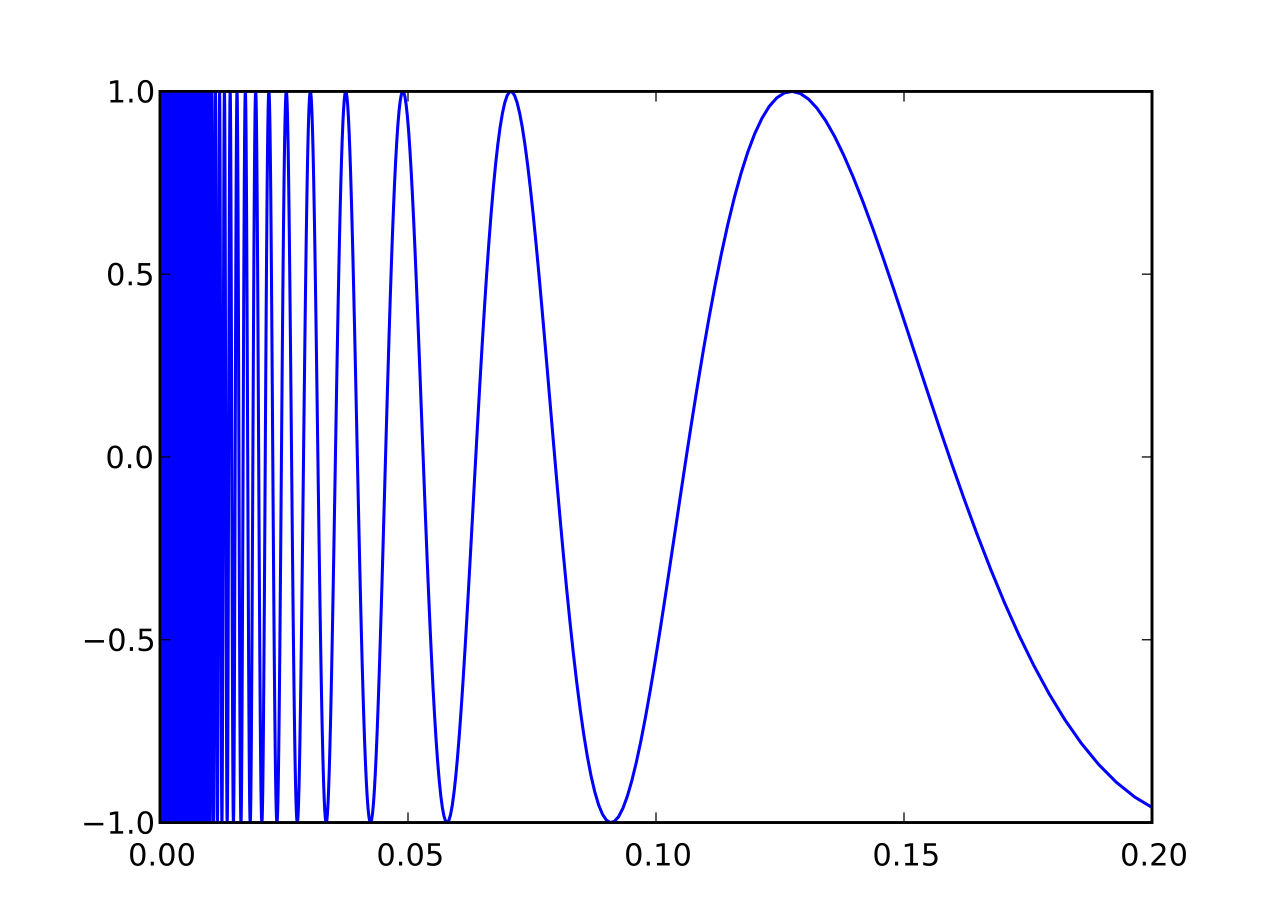
\includegraphics[width=10cm, height=8cm]{images/Topologist's_sine_curve.png}
\end{center}
\end{example}

$X$是一个连通但是不是道路连通的拓扑空间。

为什么$X$是连通的,假设$X$不连通,则存在两个disjoint开集$A$和$B$,不妨把$(0,0)$放在$A$里面,再在$B$里面取一点$(a,b)$,$A$是一个开集,所以存在一个开球$B_\varepsilon$包含$(0,0)$,尽管这个开球的$\varepsilon$可以非常小,它依然会交于$\sin\frac{1}{x}$,这个$\varepsilon$最大不会大于$d((0,0),(a,b))$,所以$\sup(\varepsilon) \leq d((0,0),(a,b))$,如果这个开球与$\sin\frac{1}{x}$的交点在$A$里面,以这个交点再做开球,则可以找到包含$(0,0)$更大开球,这不符合$\sup$的定义,如果交点在$B$里面,还是以这个交点做开球,可以找到更小的$\sup$,这也不符合$\sup$的定义,但是这些交点必须在$A$或者$B$里面,产生矛盾了,所以$X$连通.

%为什么$X$不是道路连通的呢?固定一点$T=(t,\sin\frac{1}{t})\ (t\in (0,1]))$,在定义$O=(0,0)$,假设$X$道路连通,则存在一个连续映射$\func{f}{[0,1]}{X}$,使得$f(0)=O$,$f(1) = T$. 再取$[0,1]$上的一个极限为$0$的点列$\{t_n\}$,按照连续函数的性质$\{f(t_n)\}$的极限为$f(0)$,但是实际上这个极限是不存在的,图像在趋于$0$时,在剧烈上下振荡,这个极限并不趋于$(0,0)$.

假设$X$道路连通,取两点$O=(0,0)$,$T=(\frac{1}{\pi},0)$和则存在连续映射$f(t)=(a(t),b(t))$,使得$f(0)=O$,$f(1)=T$.根据中值定理存在$0<t_1<1$使得$a(t_1)=\frac{2}{3\pi}$,接着做induction,存在$0<t_2<t_1$使得$a(t_2) = \frac{2}{5\pi}$,最后可以得到一个递减有界点列$\{t_n\} \ \lim t_n = 0$,$a(t_n) = \frac{2}{(2n+1)\pi}$,对应的$b(t_n)=(-1)^n$. 根据连续函数的性质${f(t_n)}$极限也应该存在,但是$\lim b_n$并不存在,所以$f$并不连续. (这里也可以不用中值定理,$a$是连续则$a((0,t))$也是连通的,根据我们之前的证明的性质$a((0,t))$是一个区间\rm(interval),所以我们肯定是可以找到$t' \in (0,t)$使得$a(t')$刚好位于波峰的位置,然后再induction构造$\{t_n\}$,再在每两个波峰之间取一个波谷$\{s_n\}$,它们两个都是极限都是相同的,但是$\lim b(t_n) \neq b(s_n)$(可数拓扑基下$f$连续当且仅当所有以$x$为极限的数列的像集的极限都是$f(x)$).


最后我们知道连通子集的闭包也是连通的$\overline{X} = \left\{  \left( x, \sin \tfrac{1}{x}  \right ) :  x \in (0,1] \right\} \cup \{(0,y) : y \in [-1,1]\}$,但是同样不是道路连通的.

%http://uregina.ca/~franklam/Math535/Math535_1022.pdf
\begin{proposition}
\rm 在$X$上定义一个关系$\sim$,使得$x \sim y$当且仅当$X$上存在一条从$x$到$y$的道路. 则$\sim$是一个等价关系. 每个点$x$所在的等价类$\left<x \right>$称为$x$所在的道路分支(path component).
\end{proposition}

\begin{proof}
反身性: 任取$x \in X$,有\textbf{点道路}(constant path)$f(t) = x,t \in [0,1]$.$f$连续是比较显然的,所以$x \sim x$.

对称性: 若$x \sim y$,则存在一条$x$到$y$的道路$f$,有\textbf{逆道路}(inverse path)$\overline{f}(t)=f(1-t)$. $f$是连续的,因为$t \mapsto (1-t)$是一个$[0,1]$自身的同胚,所以$y \sim x$.

传递性: 若$x \sim y, y \sim z$,则存在$x$到$y$的道路$f$和$y$到$z$的道路$g$,其中$f(1) = g(0)$,有\textbf{乘积道路}(product path or concatenation)$ab$ \[[0,1]\rightarrow X, \ t \mapsto \begin{cases} f(2t) & t \in [0,\frac{1}{2}] \\ g(2t-1) & t \in [\frac{1}{2},1] \end{cases}\],$ab$是连续的,因为在两个闭集上的限制映射都是连续的.所以$x \sim z$.
\end{proof}

下面这个定理非常有意思

\begin{theorem}
设$X$有一个道路连通覆盖(cover of path-connected subsets)$\mathscr{B}$,即$\mathscr{B}$是由道路连通子集构成的子集族,并且满足$\bigcup \mathscr{B} = X$. 如果此时$X$还有另外一个道路连通子集$A$与每一个$B \in \mathscr{B}$均相交非空,则$X$道路连通.

\begin{center}
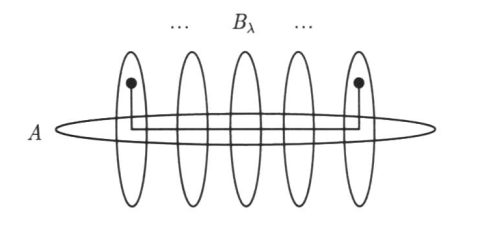
\includegraphics[width=7cm, height=4cm]{images/cover_of_path_connected_subsets.png}
\end{center}

\end{theorem}

\begin{proof}
任取$x,y \in X$,不妨设$x \in B_x \in \mathscr{B},y \in B_y \in \mathscr{B}$,则存在从$x$到某个$z_x \in B_x \cap A$的道路$f$,也存在$y$到某个$z_y \in B_y \cap A$的道路$g$,进而还存在$z_x$到$z_y$的道路,根据道路分支下的等价关系,存在$x$到$y$的道路$fc\overline{g}$.所以$X$道路连通.
\end{proof}


\newpage
\subsection{Compactness}

\rm H-Borel定理还是引理?已经不重要了都是唯一属于他的,紧致性是它的一般性推广.

\begin{definition}
若集合族$\mathcal{U}$满足$\bigcup\mathcal{U} \supseteq X$,则称之为$X$的一个\textbf{覆盖}(\rm cover). 仅含有限多个元素的覆盖称为\textbf{有限覆盖}(finite cover).若$X$的覆盖$\mathcal{U}$有子族$\mathcal{V} \subseteq \mathcal{U}$,使得$\mathcal{V}$也构成$X$的覆盖,则称$\mathcal{V}$是$\mathcal{U}$的\textbf{子覆盖}(subcover).
\end{definition}


\begin{definition}
若拓扑空间$X$的任意开覆盖有有限子覆盖,则称$X$\textbf{紧致}(\rm compact).
\end{definition}

\begin{example}
If $(X,\tpl) = \mathbb{R}$ and $A = (0,\infty)$, then $A$ is not compact.
\begin{proof}
For each positive integer $i$, let $O_i$ be the open interval $(0,1)$. Then, clearly, $A \subseteq \bigcup\limits_{i=1}^{\infty} O_i$.

But there do not exist $i_1,i_2,\cdots,i_n$ such that $A \subseteq (0,i_1) \cup (0, i_2) \cup \cdots \cup (0,i_n)$. Therefore $A$ is not compact.
\end{proof}
\end{example}

在数学分析里面E.Borel告诉我们有界闭区间是紧致的,在那个里面我似乎是用H.lebesgue的方法证明,例如给定一个闭区间$[a,b]$,去找形如$[a,x^*]$且能被有限覆盖的子集,确定$\sup(x^*)=b$,来证明整个$[a,b]$可以被有限覆盖. 这里我们用纯拓扑的方法来试着在来证一下闭区间$[0,1]$是紧致的.

\begin{proposition}
闭区间$[0,1]$是紧致的.
\end{proposition}

\begin{proof}
让$O_i,i \in I$是$[0,1]$的开覆盖. 则对任意的$x \in [0,1]$,都有一个$O_i$包含它. 由于$O_i$是开的,所以存在一个开区间$U_x \subseteq O_i$使得$x \in U_x$.

现在定义一个$[0,1]$上的子集$S$如下\[S = \Set{z}{[0,z]\ \text{可以被有限} U_x \text{所覆盖}}.\]这样如果我取$x \in S$,再取$y \in U_x$. $U_x$同时包含$x$和$y$,不妨设$x <= y$所以$[x,y] \subseteq U_x$. 我们已经有$[0,x] \subseteq \bigcup U_{x_i}$,所以$[0,y] \subseteq \bigcup U_{x_i} \cup U_x$. 这样$y \in S$.

上面这个性质告诉我们$U_x$里面的元素其实都是属于$S$的,这就意味着\[S = \bigcup\limits_{x \in S} U_x\],但是这里还是有点不太好处理,因为等式两边都有$S$. 我们在取$S$的complement:\[[0,1] \setminus S = \bigcup\limits_{x \notin S} U_x\],两者结合起来看$S$应该是一个clopen,$S$不为空,所以$S$只能是$[0,1]$.
\end{proof}

\begin{theorem}[Alexander Subbasis Theorem]
a topological space $(X,\tpl)$ is compact if and only if every subbasis cover has a finite subcoover. in other wors, if $S$ is a subbasis of topology $\tpl$, and $O_i \colon i \in I$, $I$ is an index set, is such that echo $O_i \in S$ and $X \subseteq \bigcup\limits_{i \in I} O_i$, then there is a finite subcover of $X$ by mermbers of $O_i \in I$.
\end{theorem}


\begin{definition}
若拓扑空间$X$的任意开覆盖都有一个\textbf{可数}子覆盖,则称$X$为一个\rm \textbf{Lindelöf space}.
\end{definition}

\begin{proposition}
连续映射保留紧致性. 定义$\func{f}{X}{Y}$是一个连续函数,若$A \subseteq X$紧致,则$f(A)$紧致.
\end{proposition}

\begin{proof}
取$Y$上一组开覆盖$\bigcup\limits_{\alpha \in A}V_\alpha=Y$,这样$f(A) \subseteq \bigcup\limits_{\alpha \in A}V_\alpha$.然后我们有\[A \subseteq f^{-1}(f(A)) \subseteq f^{-1}(\bigcup\limits_{\alpha \in A}V_\alpha) = \bigcup\limits_{\alpha \in A} f^{-1}(V_\alpha).\]其中$f^{-1}(V_\alpha)$开,所以就表示$A$可以被一堆开集盖住,由因为$A$紧致,所以$A \subseteq \bigcup\limits_{\alpha \in S} f^{-1}(V_\alpha)$,附带地说明了$f(A) \subseteq f(\bigcup\limits_{\alpha \in S} f^{-1}(V_\alpha) = \subseteq \bigcup\limits_{\alpha \in S} V_\alpha $.所以$f(A)$紧致.

这个证明的技巧$f(A)$的一组开覆盖的preimage,构造了一个$A$的一组开覆盖,反过来用$A$的compact性质,挑出了有限的开覆盖,再做$f$的image.
\end{proof}



\begin{example}
$X$是一个度量空间,若子集$A$紧致则$A$是一个闭集.
\end{example}

\begin{proof}
换句话说$A$紧致则$X \setminus A$开,我们的证明策略是在$X \setminus A$中固定一点$x$,然后再任取$y \in A$,分别取它们不相交的开集$x \in U_x$和$y \in U_y$(Hausdorff),最后我们只需要说明这些$\bigcap U_x$与$K$之间没有交点就行了.

开始正式证明,取$A$的一组开覆盖\[A = \bigcup\limits_{y \in A} \{y\} = \bigcup\limits_{y \in A}U_y.\]如果我们有$A$紧致,则$A \subseteq \bigcup\limits_{y \in S} U_y$. 按照我们前面的策略,我们需要取任意多对$(U_{x_y},U_y)$,其中$U_{x_y}$和$U_y$都是不相交的开集,然后我们再考虑对所有的$x \in X \setminus A$都去做这样的操作. 对于每个$x$我们都有一堆开集,但是我们肯定想要是每个$x$都只对应一个开集就好了,所以我们考虑取这堆开集的交集,但是这堆开集看起来似乎有无限对多个,如果它是有限就好了. 进一步再把所有的这样的交集并起来,它和$A$没有交点就更好了,这样这堆交集的并也就是$X \setminus A$,这就是后面我们操作的基本想法.

按照我们的基本想法来做一下. 现在$A$是紧致的,所以我们只需要关注有限个$U_y$就够了,也就是说我们也只需要取有限多个$U_{x_y}$交也就够了,记$V = \bigcap\limits_{y \in S} V_y$,其中$x \in V_y$代表$U_x$和$y$对应,这里$V$也是开集.我们现在只需要说明这个$V \cap A = \emptyset$就行了\[V \cap A \subseteq \left( \bigcap\limits_{y \in S} V_y \right) \cap \left(\bigcup\limits_{z \in S} U_z \right) = \bigcup\limits_{z \in S}\left(\bigcap\limits_{y \in S} V_y \cap U_z \right) \subseteq \bigcup\limits_{z \in S}(V_z \cap U_z) = \emptyset. \]注意最后的$V_z$这里是集合论手法$\bigcap\limits_{y \in S} V_y \subseteq V_z, z \in S$. 最后取遍所有$x$都有这样的一个开集$V$,$X \setminus A = \bigcup V$,所以$A$是一个闭集.
\end{proof}

上面这个例子更一般形式是下面的命题
\begin{proposition}
\rm Hausdorff拓扑空间的紧致子集是闭的.
\end{proposition}

\begin{proposition}
紧致空间的闭集都是紧致的.
\end{proposition}

\begin{proof}
给定$X$紧致,$A$是$X$上的一个闭集,证明还是用集合论的手法:\[X = A \cup X \setminus A.\]取$A$上的一组开覆盖$O_i,i \in I$,所以$X = \left( \bigcup\limits_{i \in I} O_i \right) \cup X \setminus A$,其中$X \setminus A$开,所以整体上是$X$的一组开覆盖,我们可以从这组开覆盖里面来调一组有限开覆盖. 首先$X \setminus A \cap \left( \bigcup\limits_{i \in I} O_i \right)= \emptyset$,所以$X \setminus A$得先挑出来,也就是说我们可以从$O_i,i \in I$里面挑有限多个出来覆盖$A$,即$A$紧致.
\end{proof}

把Heine-Borel Theorem推广到更一般的情况上.
\begin{proposition}
\rm 度量空间$X$上子集$A$紧致,则$A$有界闭(closed and bounded).
\end{proposition}

\begin{proof}
度量空间是一个Hausdorff空间,$A$紧致,所以$A$是闭的. 这一点前面已经证明了.

$A$紧致,所以它可以被有限的开集盖住,为了说明$A$有界,我们只需要找一个更大的开球把$A$盖住就可以了. 现在来严格证明下,找一个更大开球时,首先要我们需要确定center点,设这个点为$x_0$,我们定义一个映射如下\[\func{f}{(A,\tpl)}{\mathbb{R}}, f(a) = d(a,x_0), a \in A.\]用表示$A$中一点到$x_0$的距离. 其中$\tpl$表示$A$是$X$子空间诱导出来的拓扑. 明显地,这个$f$是一个连续映射(可以利用性质就简单检验一下),所以$f(A)$紧致,$\mathbb{R}$的紧致子集是有界闭的,也就是存在一个$M$使得$\forall a \in A, f(a) \leq M$,那么现在我们要找的这个更大的开球的半径也可以确定了,只需要取$r = 2M$即可,利用三角不等式我们知道$d(a_1,a_2)<2M$.  
\end{proof}

上述证明里面用$f$可以更一般化.

\begin{lemma}
给定一个连续映射$\func{f}{X}{\mathbb{R}}$,若$X$是一个紧致空间,则$f(X)$有界(上下界).
\end{lemma}

\begin{proof}
连续映射保留紧致,所以$f(X)$紧致,而$\mathbb{R}$上的紧致子集有界闭.
\end{proof}


\begin{lemma}
给定两个拓扑空间$X$和$Y$,$K$是$Y$上的一个紧致子集,$U$是乘积空间$X \times Y$上的一个开集. 定义集合$V = \Set{x \in X}{\{x\} \times K \subset U}$,则$V$是一个$X$上的一个开集.
\end{lemma}
%https://www.maths.tcd.ie/~dwilkins/Courses/221/Compact.pdf
\begin{proof}
证明$V$开的主旋律是给每个$x$都找一个含于$V$的开集. 假设$V$非空,fixed $V$中一点$x$. 对于任意$y \in Y$,存在一对开集$D_y \subseteq  X$和$E_y \subseteq Y$, 对应$(x,y) \in D_y \times E_y \subseteq U$. 因为$K$紧致,所以恒存在一个有限的开覆盖$K \subseteq E_{y_1},E_{y_2},\cdots,E_{y_n}$,其中$y_1,y_2,\cdots,y_n \in Y$(这里用到$K$紧致这个条件是因为不知道$E_y$是否有限).考虑$x \in N_x = D_{y_1} \cap D_{y_2} \cap \cdots \cap D_{y_n}$,其中$D_{y_i}$对应前面pair中的$D_y$. 自然地考虑\[N_x \times K \subseteq \bigcup\limits_{i}^{n}\left( N_x \times E_{y_i} \right) \subseteq \bigcup\limits_{i}^{n}\left( D_{y_i} \times E_{y_i} \right) \subseteq U.\]所以$N_x \subseteq U$,每个$x$都有这样的一个开集,从而$V = \bigcup N_x$.
\end{proof} 

\begin{theorem}[Tychonoff's Theorem for Finite Products]
若$X_1,X_2,\cdots,X_n$都是紧致空间,则有限乘积空间$\prod\limits^{n} X_i$也是紧致的.
\end{theorem}

\begin{proof}
It suffice to prove that the product of two compact topological spaces, then by induction.

给定两个紧致空间$X$和$Y$,$O_i,i \in I$是它们的一组开覆盖,我们目标是可以从里面调出一组有限开覆盖出来.

还是先fixed一点$x \in X$,则$\{x\} \times Y$是$X \times Y$的一个紧致子集,因为把$y \in Y$映射到$(x,y)$这是一个homoemophism,$Y$紧致所以$\{x\} \times Y$紧致. 进一步这里存在$\{x\} \times Y$的一组有限开覆盖$\bigcup O_{i_k}$. 同样地这里也用$V_x$来表示形如$\{x'\} \times Y \subset \bigcup O_{i_k}$这样的所有$x' \in X$. 根据前面的Lemma,$\bigcup O_{i_k}$是一个$X \times Y$上的开集,所以$V_x$是一个开集. 

现在我们知道了$V_x \times Y$可以被$\bigcup O_{i_k}$有限覆盖. 但是$X$还没有被盖住,再用$\{V_x \colon x \in X\}$作为$X$的一组开覆盖,由于$X$紧致,所以只需要有限多个$V_{x_j}$就可以盖住. $X \times Y = \bigcup \left( V_{x_j} \times Y \right)$,而$V_{x_j} \times Y$前面已经证明可以被有限多个$O_{i_k}$盖住,所以$X \times Y$也可以被有限多个$\bigcup\bigcup O_{i_k}$盖住,$X \times Y$紧致.
\end{proof}


\begin{theorem}[Generalized Heine-Borel Theorem]
$\mathbb{R}^{n},n \geq 1$上的子集$A$紧致当且仅当$A$有界闭.
\end{theorem}

\end{document}



